% \chapter{Omitted theory}
% \label{app:theory}
% \todo{Would like feedback if this is necessary and/or a good way of including extra theory.}
% \section*{Why  $\bm Q$ is sparse in a GMRF}
% In a GMRF, we have the graph $\mathcal G = (V, E)$ with vertices $V$ and edges $E$ and the random vector $\bm X=\{x_\nu\}_{\nu \in V}$. Furthermore, $\bm X \sim \mathcal N(\bm 0,\bm Q^{-1})$ and satisfies the Markov property $x_j \perp x_{i} | x_{-ij}$, where $i$ and $j$ are not neighboring vertices in the graph, and the notation $ x_{-ij}$ are all $x_k \in \{x_\nu\}_{\nu \in V \setminus \{i,j\}}$. Thus, by construction, we get that $\bm Q_{ij}=0$, so that $\bm Q$ is sparse. 

% \section*{Genetic groups in animal models}
% We can partition the additive genetic effect into a term capturing individual variation and another capturing immigrant genes, $a_i = u_i + gq_i$. Here, $u_i$ is the deviation from $i$ to the other native group, $q_i$ is the expected contribution of immigrant genes and $g$ is an immigration coefficient, computed as the difference between the native population and the immigrants' genetic group. Notice that this means that the $u_i$ are relative to the founder population.

% % \section*{Distribution specific variance functions}
% % For instance, in a binary logit model, $\frac{e^x}{1+e^x}\left(1-\frac{e^x}{1+e^x}\right) = \frac{\partial}{\partial x}g^{-1}(x)$. For the probit case, the distribution-specific variance function is $\Phi(x)(1-\Phi(x))$.

% \section*{Decomposition of relatedness matrix}
% We also consider the decomposition $\bm A = \bm L \bm D \bm L^\top$, in which $\bm L$ is lower triangular and contains information about what genes the individual derives from its ancestors. The diagonal matrix $\bm D$ contains within-family additive genetic variance. From this decomposition, we can construct $\bm A$ with little time and memory complexity using the algorithm described in \textcite{luo1992computing}. Thus, using the pedigree we can encode relatedness into the linear predictor of the animal model. 


\chapter{Additional plots}
% An initial step is to examine the generated pedigree and in particular the relatedness of the different individuals. \autoref{fig:relatedness offdiagonal} displays the off-diagonal values of the relatedness matrices, where a high concentration around larger values would indicate a large degree of relatedness.

\begin{figure}
    \centering
    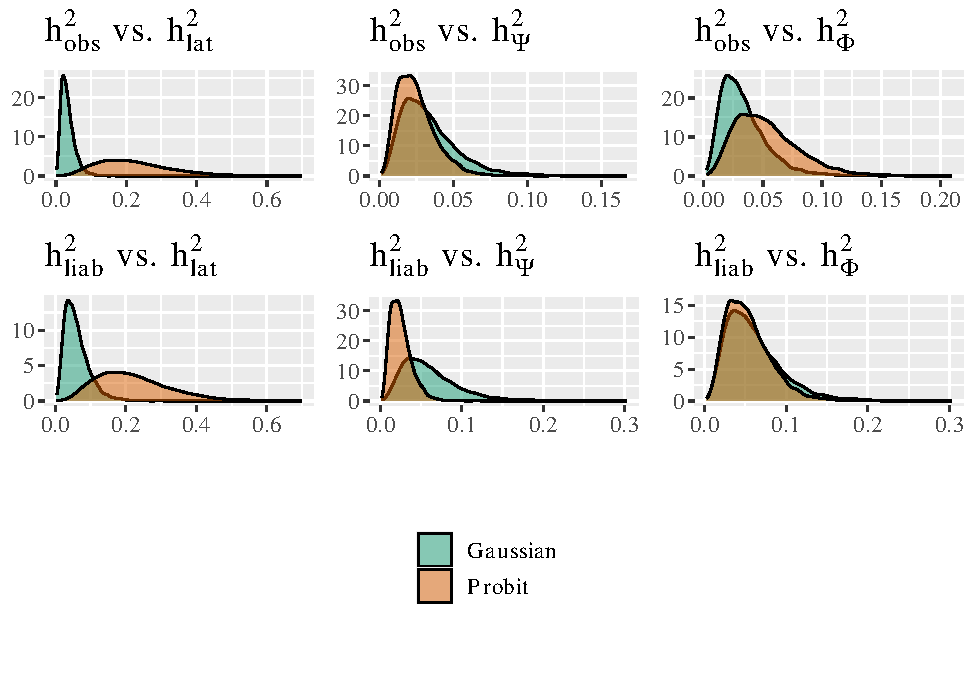
\includegraphics[width=0.8\textwidth]{figures/grid_application_gaussian_vs_binom.pdf}
    \caption[Posterior heritability for application data in different scales]{Posterior distributions of estimated heritability for the Gaussian and probit model, in the application data. The densities are reported in a grid comparing each different type of scale to each other. That is, for both scales for the Gaussian model, we compare the posterior heritability with the probit model for its three different scales. The resulting 3$\times$2 grid shows how they act comparatively.}
    \label{fig:application gaussian vs binomial}
\end{figure}

\begin{figure}
    \centering
    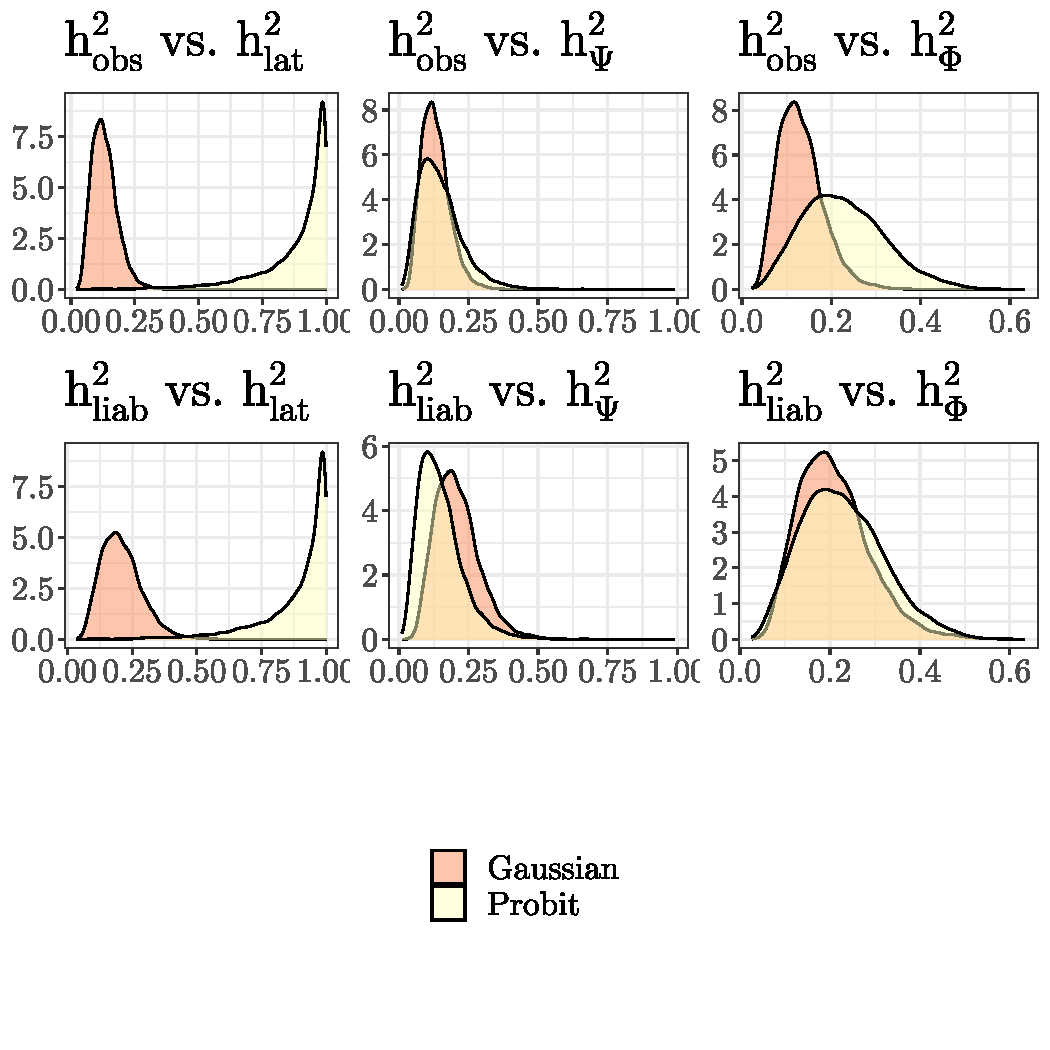
\includegraphics[width=0.8\textwidth]{figures/grid_simulation_gaussian_vs_binom.pdf}
    \caption[Posterior heritability for simulation data in different scales]{Posterior distributions of estimated heritability for the Gaussian and probit model, in the simulation data with $\sigma^2_A=0.5$ and $\sigma^2_E=1$. The densities are reported in a grid comparing each different type of scale to each other. That is, for both scales for the Gaussian model, we compare the posterior heritability with the probit model for its three different scales. The resulting 3$\times$2 grid shows how they act comparatively.}
    \label{fig:simulatino gaussian vs binomial}
\end{figure}

\begin{figure}
    \centering
    \begin{subfigure}{0.49\textwidth}
    \caption{$\beta=1$, $\sigma^2_A=10$, $\sigma^2_E=1$, $p=0.5$}
    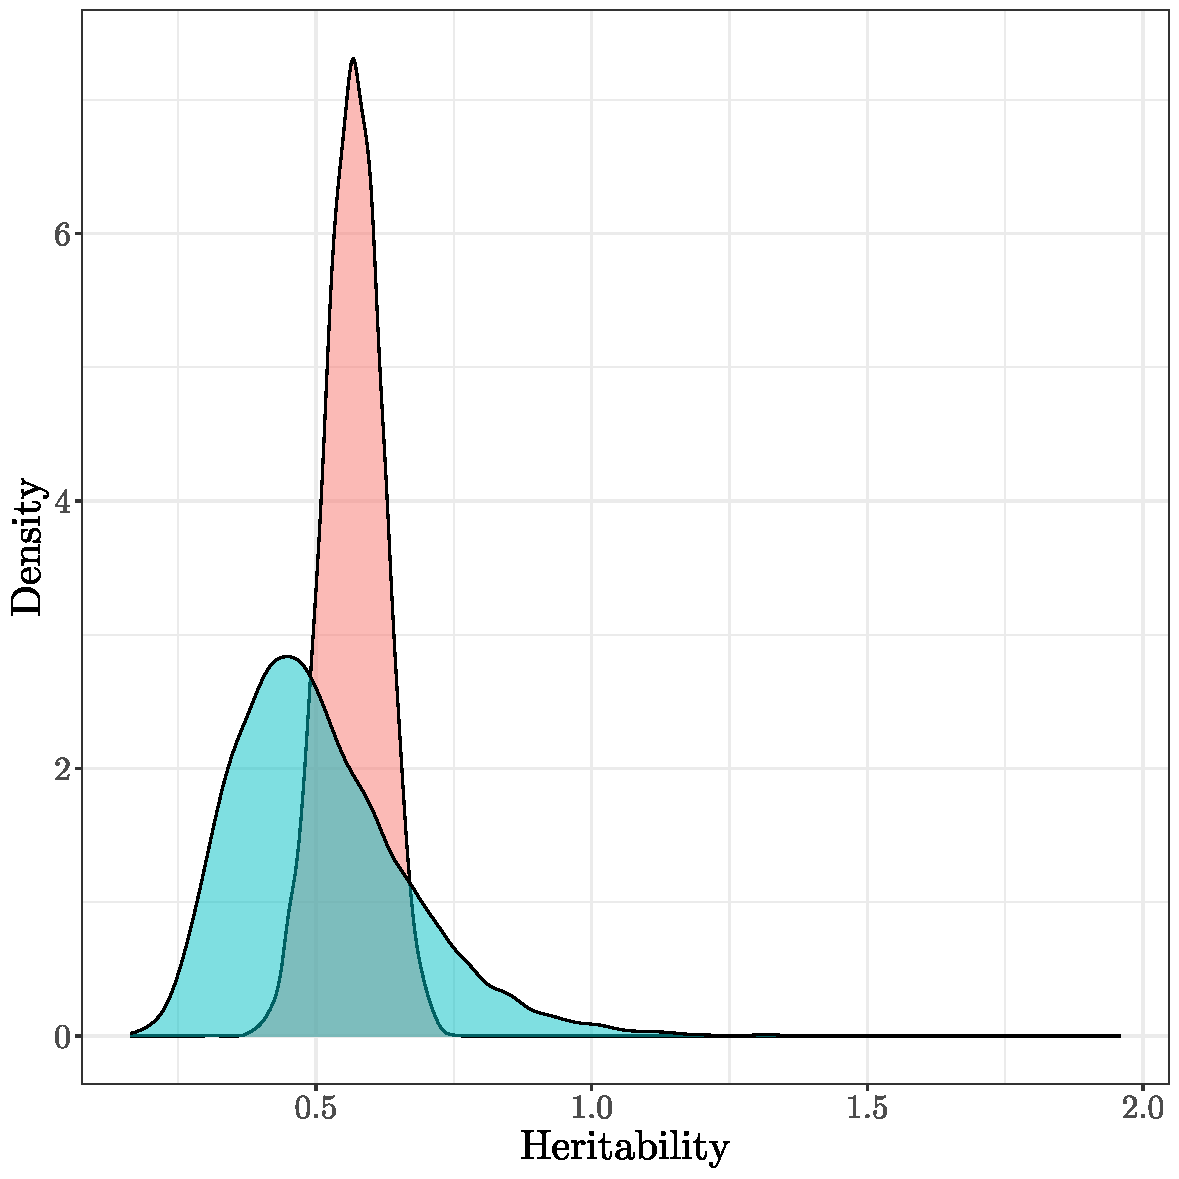
\includegraphics[width=\textwidth]{figures/fixedeffects_gaussian_probit_sA10_p_5_beta_1.pdf}
    \end{subfigure}
    \begin{subfigure}{0.49\textwidth}
    \caption{$\beta=5$, $\sigma^2_A=10$, $\sigma^2_E=1$, $p=0.5$}
    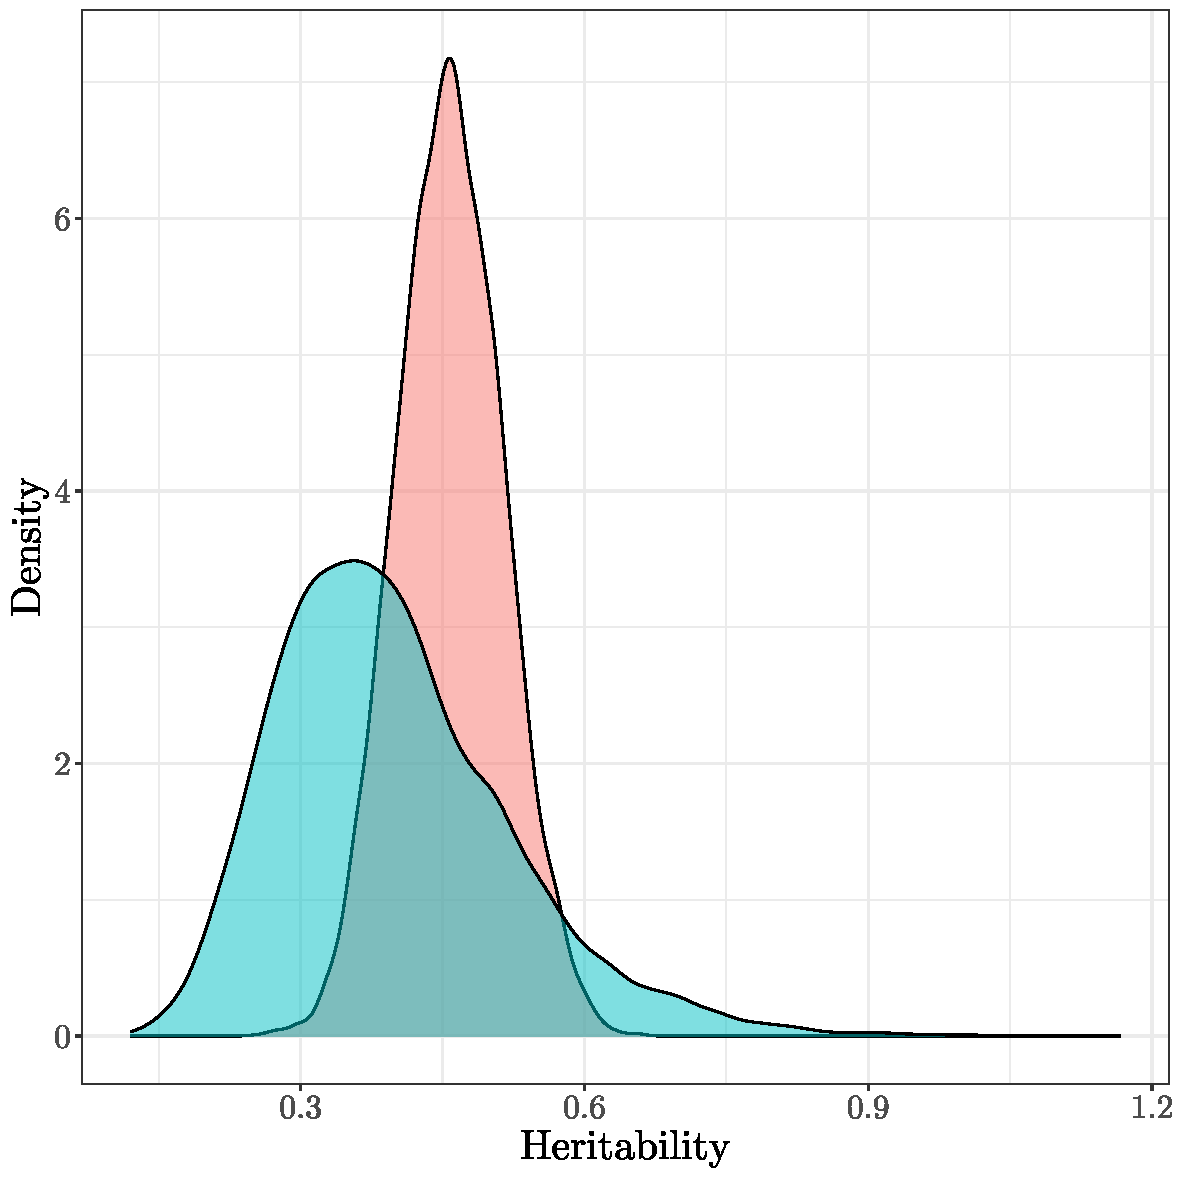
\includegraphics[width=\textwidth]{figures/fixedeffects_gaussian_probit_sA10_p_5_beta_5.pdf}
    \end{subfigure}
    \begin{subfigure}{0.49\textwidth}
    \caption{$\beta=1$, $\sigma^2_A=500$, $\sigma^2_E=1$, $p=0.5$}
    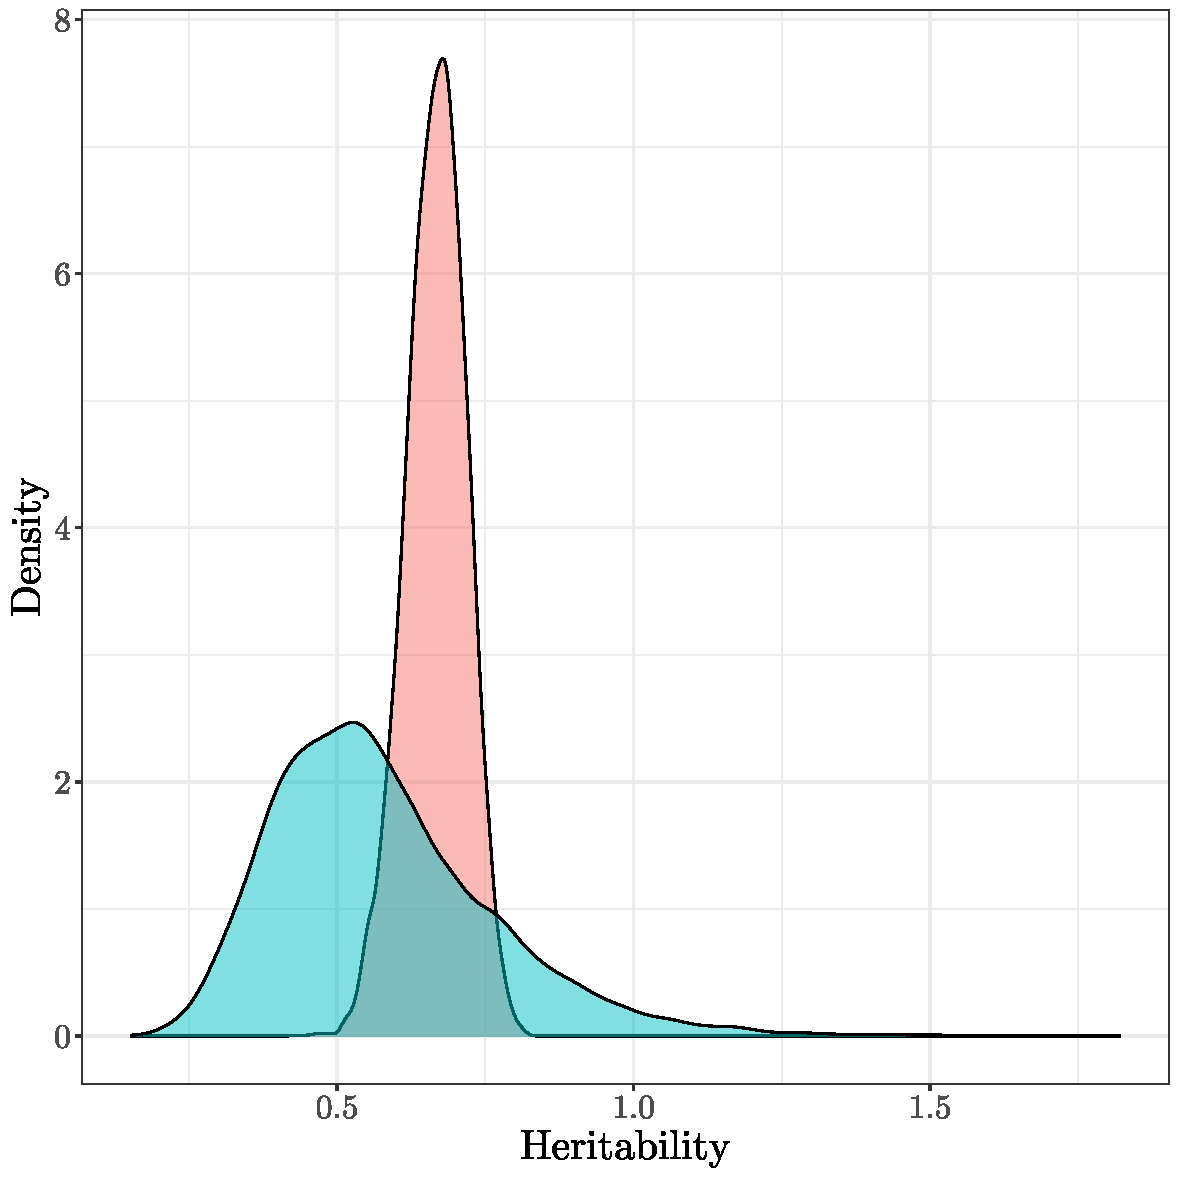
\includegraphics[width=\textwidth]{figures/fixedeffects_gaussian_probit_sA500_p_5_beta_1.pdf}
    \end{subfigure}
    \begin{subfigure}{0.49\textwidth}
    \caption{$\beta=5$, $\sigma^2_A=500$, $\sigma^2_E=1$, $p=0.5$}
    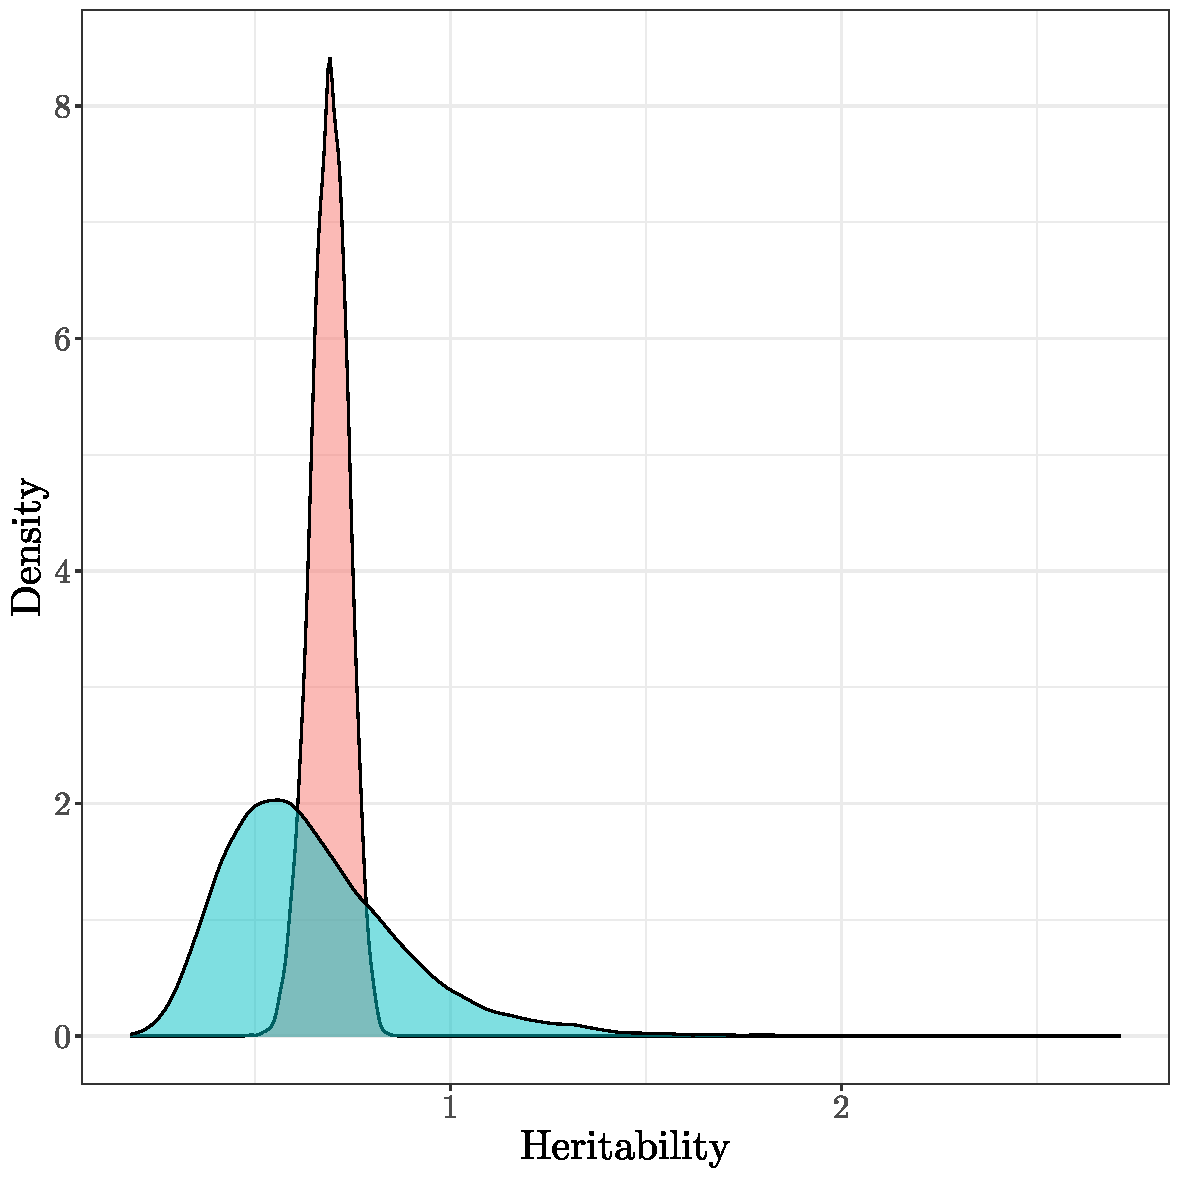
\includegraphics[width=\textwidth]{figures/fixedeffects_gaussian_probit_sA500_p_5_beta_5.pdf}
    \end{subfigure}
    \begin{subfigure}{0.6\textwidth}
    
\includegraphics[width=\textwidth]{figures/fixedeffects_gaussian_probit_legend.pdf}
    \end{subfigure}
    \caption[$h^2$ for fixed effects with varying $\beta$]{Posterior heritability for simulations with fixed effects on observation-scale, varying on $\beta$ between $1$ and $5$ across the columns, and between $\sigma^2_A=10$ and $500$ across the rows.}
    \label{fig:fixedeffects varying betas}
\end{figure}

\chapter{Exploratory Data Analysis}
\label{app:EDA}
\hypertarget{data-frame-overview}{%
\section*{Data frame overview}\label{data-frame-overview}}

\hypertarget{pedigree}{%
\subsection*{Pedigree}\label{pedigree}}

The first object is \texttt{d.ped} which contains the pedigree
information.

\begin{Shaded}
\begin{Highlighting}[]
\FunctionTok{summary}\NormalTok{(d.ped)}
\end{Highlighting}
\end{Shaded}

\begin{verbatim}
##     ninecode             gendam             gensire         
##  Min.   :109137448   Min.   :109137468   Min.   :109137448  
##  1st Qu.:146164012   1st Qu.:146130794   1st Qu.:146130313  
##  Median :176124850   Median :176124382   Median :176124004  
##  Mean   :196520240   Mean   :188116000   Mean   :185463038  
##  3rd Qu.:243185045   3rd Qu.:226189260   3rd Qu.:226189228  
##  Max.   :999999999   Max.   :999999999   Max.   :266176829  
##                      NA's   :59          NA's   :59
\end{verbatim}

It has columns \emph{ninecode}, \emph{gendam}, and \emph{gensire}.
The first column cannot be \texttt{NA} and is the unique identifier for
an individual, whereas \texttt{gendam} and \texttt{gensire} are
references (foreign keys) to the known maternal and paternal link,
respectively. Both of these columns have 59 NAs. In fact, these NAs
overlap completely since they are the founder population with no defined
paternal or maternal link:

\begin{Shaded}
\begin{Highlighting}[]
\NormalTok{d.ped[}\FunctionTok{is.na}\NormalTok{(d.ped}\SpecialCharTok{$}\NormalTok{gendam), }\StringTok{"gensire"}\NormalTok{]}
\end{Highlighting}
\end{Shaded}

\begin{verbatim}
##  [1] NA NA NA NA NA NA NA NA NA NA NA NA NA NA NA NA NA NA NA NA NA NA NA NA NA
## [26] NA NA NA NA NA NA NA NA NA NA NA NA NA NA NA NA NA NA NA NA NA NA NA NA NA
## [51] NA NA NA NA NA NA NA NA NA
\end{verbatim}

We see that \emph{gensire} is NA for all instances where \emph{gendam}
is also NA. This is the founder population with no defined parental
linkage.

\hypertarget{d.q}{%
\subsection*{d.Q}\label{d.q}}

This table has the columns \emph{g1}, \emph{foc0} and \emph{ninecode}
(ID).

\begin{Shaded}
\begin{Highlighting}[]
\FunctionTok{head}\NormalTok{(d.Q)}
\end{Highlighting}
\end{Shaded}

\begin{verbatim}
##   foc0 g1  ninecode
## 1    1  0 109137407
## 2    1  0 109137408
## 3    1  0 109137418
## 4    1  0 109137420
## 5    1  0 109137421
## 6    1  0 109137425
\end{verbatim}

Considering only the first results, it might seem like \texttt{foc0} and
\texttt{g1} are binary/categorical variables, but plotting the values
across indices show that the order of the rows are structured so that
they start at 1 and 0 respectively.

\begin{Shaded}
\begin{Highlighting}[]
\FunctionTok{par}\NormalTok{(}\AttributeTok{mfrow =} \FunctionTok{c}\NormalTok{(}\DecValTok{1}\NormalTok{, }\DecValTok{2}\NormalTok{))}
\FunctionTok{plot}\NormalTok{(d.Q}\SpecialCharTok{$}\NormalTok{g1, }\AttributeTok{main =} \StringTok{"g1"}\NormalTok{)}
\FunctionTok{plot}\NormalTok{(d.Q}\SpecialCharTok{$}\NormalTok{foc0, }\AttributeTok{main =} \StringTok{"foc0"}\NormalTok{)}
\end{Highlighting}
\end{Shaded}

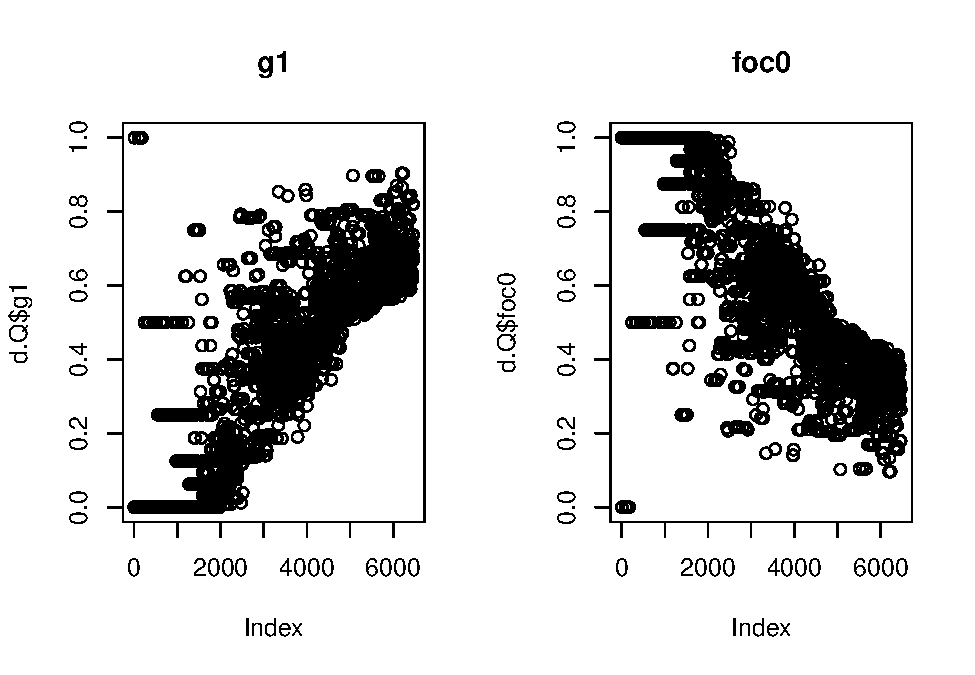
\includegraphics{EDA_files/figure-latex/unnamed-chunk-2-1.pdf}

We can also look at the correlation between these two values

\begin{Shaded}
\begin{Highlighting}[]
\FunctionTok{cor}\NormalTok{(d.Q}\SpecialCharTok{$}\NormalTok{foc0, d.Q}\SpecialCharTok{$}\NormalTok{g1)}
\end{Highlighting}
\end{Shaded}

\begin{verbatim}
## [1] -1
\end{verbatim}

Hence, we have a very strong negative correlation here. We can also look
at the individuals whose ID were in the \emph{founder population}:

\begin{Shaded}
\begin{Highlighting}[]
\NormalTok{founder\_population.id }\OtherTok{\textless{}{-}}\NormalTok{ d.ped[}\FunctionTok{is.na}\NormalTok{(d.ped}\SpecialCharTok{$}\NormalTok{gendam), }\StringTok{"ninecode"}\NormalTok{]}
\FunctionTok{table}\NormalTok{(d.Q[}\FunctionTok{which}\NormalTok{(d.Q}\SpecialCharTok{$}\NormalTok{ninecode }\SpecialCharTok{\%in\%}\NormalTok{ founder\_population.id),}
          \FunctionTok{c}\NormalTok{(}\StringTok{"foc0"}\NormalTok{, }\StringTok{"g1"}\NormalTok{)])}
\end{Highlighting}
\end{Shaded}

\begin{verbatim}
##     g1
## foc0  0  1
##    0  0 33
##    1 26  0
\end{verbatim}

The values seem to be relatively balanced between \(0\) and \(1\) in the
founder population. This supports the idea that they measure the
immigration contribution to the genetic composition of the individuals.
All immigrant individuals are completely immigrant, have no pedigree and
are thus part of the founder population. The latter are those who are
the ``initial'' natives on the island, meaning that their values must be
exactly zero.

\hypertarget{ped.prune}{%
\subsection*{ped.prune}\label{ped.prune}}

This is a pruned pedigree, only considering the 1993-2018 observations
but also combining the knowledge of the 1975-1992 observations into
them.

\hypertarget{qg.data.gg.ind}{%
\subsection*{qg.data.gg.ind}\label{qg.data.gg.ind}}

This object has the following shape:

\begin{Shaded}
\begin{Highlighting}[]
\FunctionTok{head}\NormalTok{(qg.data.gg.inds)}
\end{Highlighting}
\end{Shaded}

\begin{verbatim}
##    ninecode natalyr sex.use nestrec surv.ind.to.ad brood.date sex.use.x1
## 1 111111112    2012       0    3086              0        120          1
## 2 111111121    2015       0    3237              0        141          1
## 3 143173366    1993       1    1838              1         96          1
## 4 143173381    1993       2    1867              1        102          2
## 5 143173382    1993       1    1867              0        102          1
## 6 143173384    1993       1    1851              0        102          1
##       f.coef      foc0        g1 natalyr.no sex
## 1 0.11155218 0.4085679 0.5914321         38   0
## 2 0.04814660 0.3299752 0.6700248         41   0
## 3 0.05108643 0.5283203 0.4716797         19   0
## 4 0.03125000 0.6250000 0.3750000         19   1
## 5 0.03417969 0.4335938 0.5664062         19   0
## 6 0.02148438 0.6328125 0.3671875         19   0
\end{verbatim}

The response variable we will use is \texttt{surv.ind.to.ad}. Below are
some elementary properties of the data.

\begin{verbatim}
## [1] "Earliest year: 1993"
\end{verbatim}

\begin{verbatim}
## [1] "Number not survived: 1817" "Number survived: 661"
\end{verbatim}

\begin{verbatim}
## [1] "natal year correlation: 1"
\end{verbatim}

\begin{verbatim}
## [1] "correlation between sex and sex.x1: 0.842997540673555"
\end{verbatim}

An overview of the columns:

\begin{itemize}
\tightlist
\item
  \emph{ninecode}: Individual ID
\item
  \emph{natalyr}: The year the individual was born, e.g.~2015.
\item
  \emph{sex.use}: \textbf{Not in use}
\item
  \emph{nestrec}: ID for nest number
\item
  \emph{brood.date}: Day of the year when the first offspring in
  individuals nest hatched
\item
  \emph{sex.use.x1}: Sex of individual, 1 or 2
\item
  \emph{f.coef}: Inbreeding coefficient
\item
  \emph{foc0}: ``How foreign'' individual is, related to \texttt{f.coef}
\item
  \emph{g1}: Inverse of \emph{foc0}.
\item
  \emph{natalyr.no}: The same as the natal year, starting with 1974 as 0
  (2015=41).
\end{itemize}

\hypertarget{vizualization-of-juvenile-survival}{%
\section*{Vizualization of juvenile
survival}\label{vizualization-of-juvenile-survival}}

We will have a look at how the response, juvenile survival, relates to
the other covariates in our data.

First, we look at sex:

\begin{verbatim}
## Warning: package 'ggplot2' was built under R version 4.2.2
\end{verbatim}

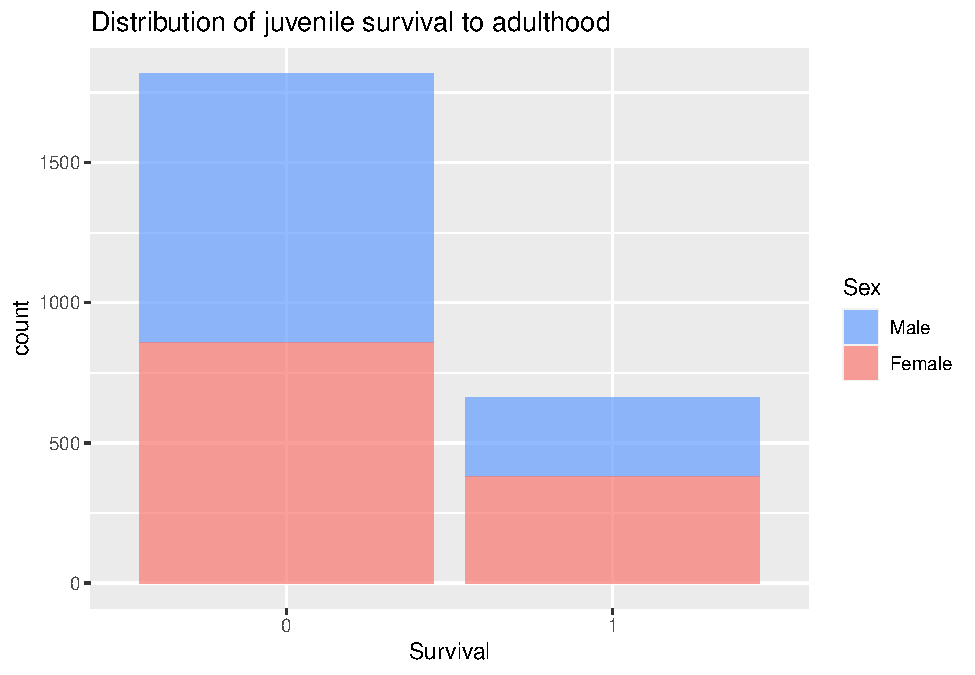
\includegraphics{EDA_files/figure-latex/unnamed-chunk-7-1.pdf}

It seems like the sex in relation to survival is relatively balanced
here. We can note that it seems like a larger portion of those surviving
are females. Next, we examine the breeding coefficient.

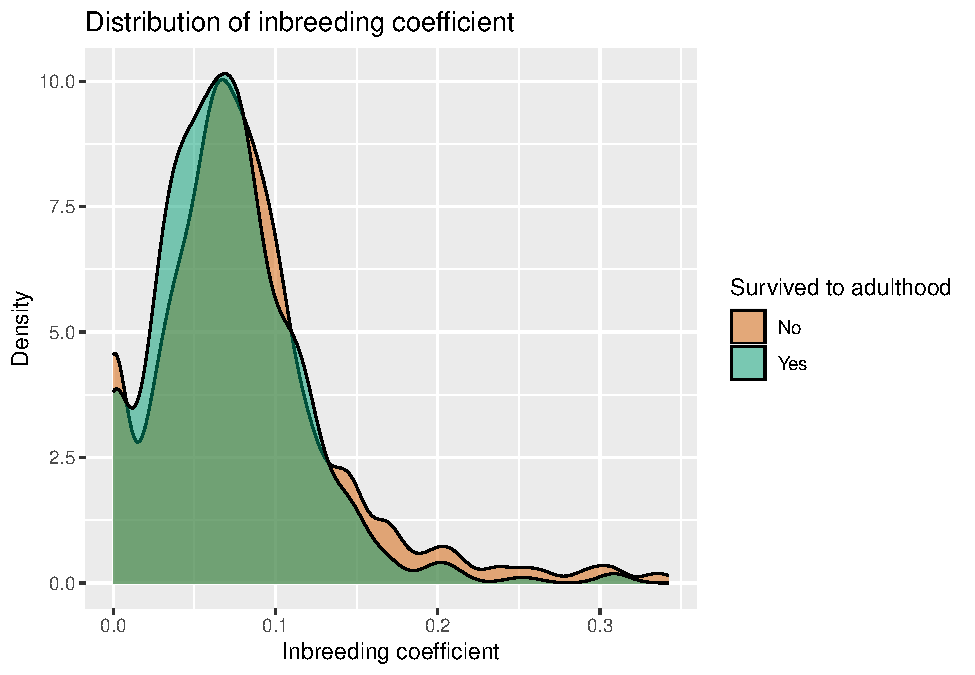
\includegraphics{EDA_files/figure-latex/unnamed-chunk-8-1.pdf}

Here we see that survival is a bit more skewed toward lower inbreeding
coefficients. We may also plot the proportion of individuals who survived
over each year:

\begin{verbatim}
## `geom_smooth()` using method = 'loess' and formula = 'y ~ x'
\end{verbatim}

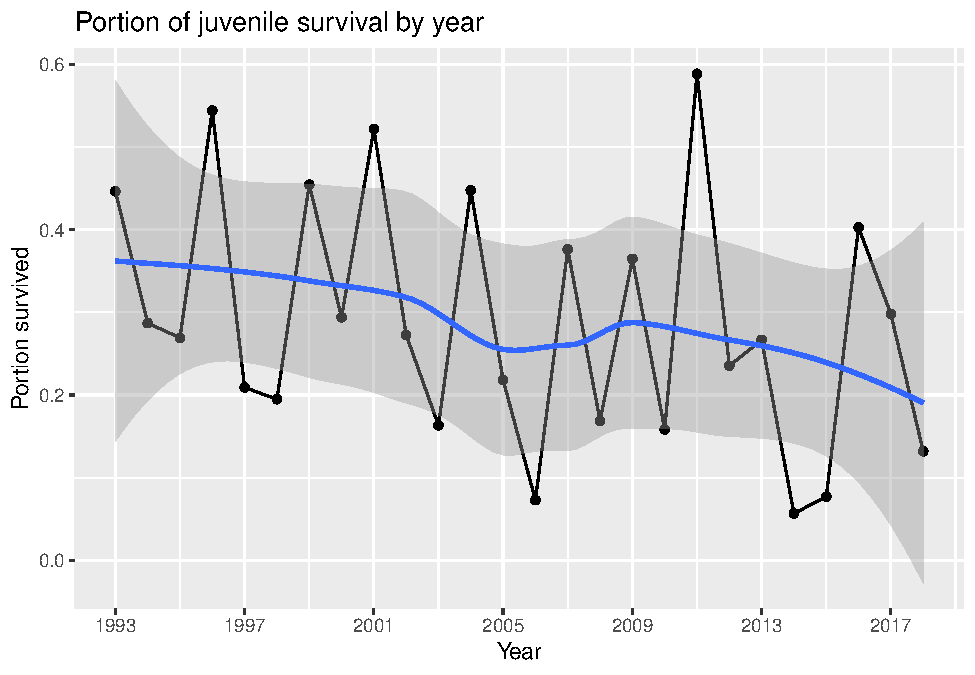
\includegraphics{EDA_files/figure-latex/unnamed-chunk-9-1.pdf}

There seems to be very little trending over the years, but possibly a
small negative trend. We also examine if there is some correspondence
between genetic group coefficient (\texttt{g1}) and juvenile survival.

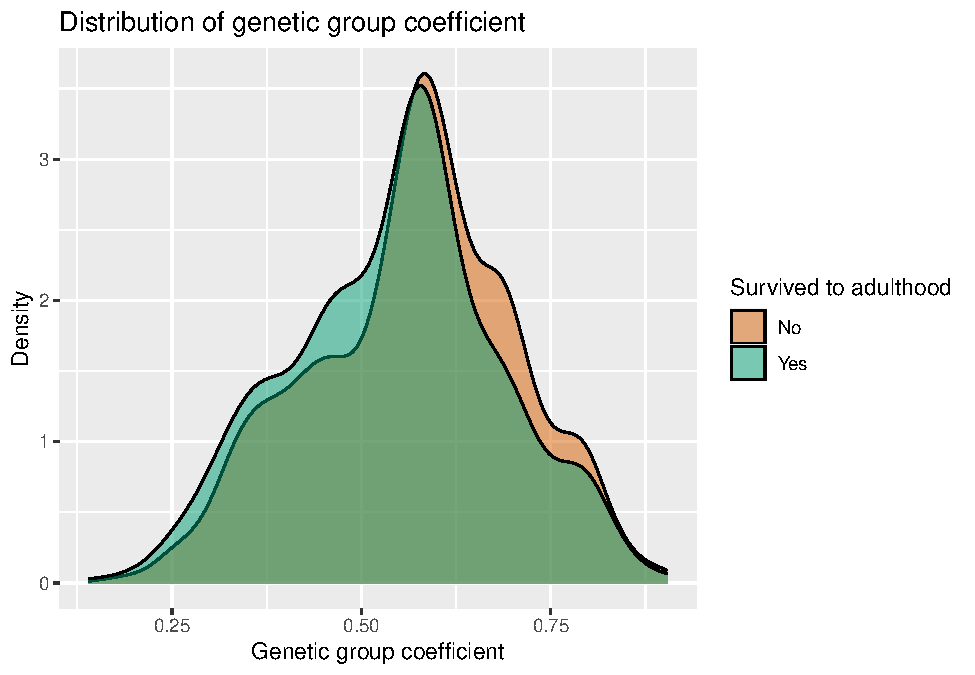
\includegraphics{EDA_files/figure-latex/unnamed-chunk-10-1.pdf}

This shows a similar result to the inbreeding coefficient, namely a skew
towards the right (lower values of coefficient) in the group that
survived. Finally, we plot the survival probability based on brood date:

\begin{verbatim}
## `geom_smooth()` using method = 'loess' and formula = 'y ~ x'
\end{verbatim}

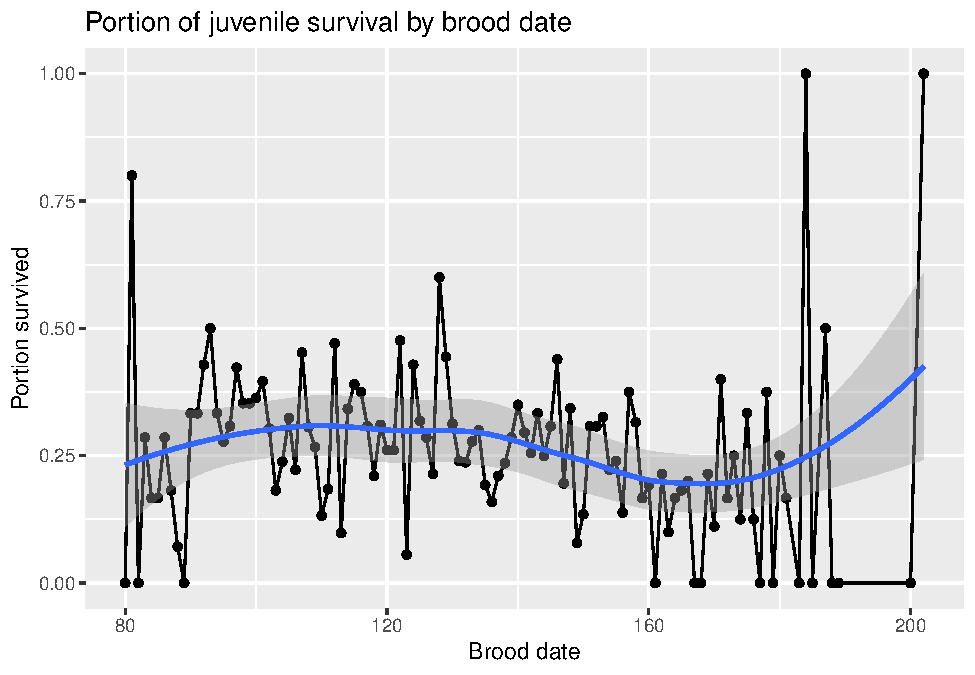
\includegraphics{EDA_files/figure-latex/unnamed-chunk-11-1.pdf}

This last plot seems to indicate that survival is relatively stable and
somewhat decreasing for those hatched relatively late. For the largest
values of brood date, we get an increasing trend but also much
uncertainty since not that many were hatched this late.

\chapter{Patching \texttt{rbv}}
\label{app:rbv-patch}
\hypertarget{how-the-bug-arises}{%
\section*{How the bug arises}\label{how-the-bug-arises}}

The function \texttt{rbv} generates random breeding values based on a
pedigree. The pedigree must either be a data frame with columns
\emph{id, dam, sire}, or a \texttt{phylo} object. The issue arises when
using GeneticsPed to generate the pedigree since this returns a
multi-class object rather than just one single object.

\hypertarget{minimal-viable-product-to-reproduce-issue}{%
\section*{Minimal viable product to reproduce
issue}\label{minimal-viable-product-to-reproduce-issue}}

\begin{Shaded}
\begin{Highlighting}[]
\FunctionTok{library}\NormalTok{(GeneticsPed)}
\end{Highlighting}
\end{Shaded}

\begin{verbatim}
## Warning: package 'GeneticsPed' was built under R version 4.2.2
\end{verbatim}

\begin{verbatim}
## Loading required package: MASS
\end{verbatim}

\begin{verbatim}
## 
## Attaching package: 'GeneticsPed'
\end{verbatim}

\begin{verbatim}
## The following object is masked from 'package:stats':
## 
##     family
\end{verbatim}

\begin{Shaded}
\begin{Highlighting}[]
\FunctionTok{library}\NormalTok{(MCMCglmm)}
\end{Highlighting}
\end{Shaded}

\begin{verbatim}
## Loading required package: Matrix
\end{verbatim}

\begin{verbatim}
## Warning: package 'Matrix' was built under R version 4.2.2
\end{verbatim}

\begin{verbatim}
## Loading required package: coda
\end{verbatim}

\begin{verbatim}
## Warning: package 'coda' was built under R version 4.2.2
\end{verbatim}

\begin{verbatim}
## Loading required package: ape
\end{verbatim}

\begin{verbatim}
## Warning: package 'ape' was built under R version 4.2.2
\end{verbatim}

\begin{Shaded}
\begin{Highlighting}[]
\NormalTok{ped0 }\OtherTok{\textless{}{-}} \FunctionTok{generatePedigree}\NormalTok{(}\AttributeTok{nId =} \DecValTok{100}\NormalTok{, }\AttributeTok{nGeneration =} \DecValTok{9}\NormalTok{, }
                         \AttributeTok{nFather =} \DecValTok{50}\NormalTok{, }\AttributeTok{nMother =} \DecValTok{50}\NormalTok{)}
\NormalTok{pedigree }\OtherTok{\textless{}{-}}\NormalTok{ ped0[ , }\FunctionTok{c}\NormalTok{(}\DecValTok{1}\NormalTok{,}\DecValTok{3}\NormalTok{,}\DecValTok{2}\NormalTok{)]}
\FunctionTok{names}\NormalTok{(pedigree) }\OtherTok{\textless{}{-}} \FunctionTok{c}\NormalTok{(}\StringTok{"id"}\NormalTok{, }\StringTok{"dam"}\NormalTok{, }\StringTok{"sire"}\NormalTok{)}
\FunctionTok{attr}\NormalTok{(pedigree, }\StringTok{"class"}\NormalTok{) }\CommentTok{\# Contains 2 classes}
\end{Highlighting}
\end{Shaded}

\begin{verbatim}
## [1] "Pedigree"   "data.frame"
\end{verbatim}

Trying to use rbv will end in an error

\begin{Shaded}
\begin{Highlighting}[]
\NormalTok{u }\OtherTok{\textless{}{-}} \FunctionTok{rbv}\NormalTok{(pedigree, }\FloatTok{0.4}\NormalTok{)}
\end{Highlighting}
\end{Shaded}

The error code is

\begin{verbatim}
Error in if (attr(pedigree, "class") == "phylo") { : 
  the condition has length > 1
\end{verbatim}

\hypertarget{patching-the-issue}{%
\section*{Patching the issue}\label{patching-the-issue}}

The only line required to change is in \texttt{rbv.R}, and is the fifth
line. Simply change it from

\begin{verbatim}
if(attr(pedigree, "class")=="phylo"){ped=FALSE}
\end{verbatim}

and change it to:

\begin{verbatim}
if(any(attr(pedigree, "class")=="phylo)){ped=FALSE}
\end{verbatim}

Then, rebuild the modified package. A patched tarball file is available
on Github
\href{https://github.com/frederni/TMA4900-MasterThesis/blob/main/MCMCglmm-rbv-patch.tar.gz}{here}.


\chapter{R script}
\label{app:Rmd script}
\hypertarget{r-code-acknowledgements}{%
\section*{R code acknowledgements}\label{r-code-acknowledgements}}

The application dataset and a large portion of data preprocessing is
provided by Jane Reid. The re-implementation into INLA is also largely
based on the work from Stefanie Muff.

\hypertarget{data-loading}{%
\section*{Data loading}\label{data-loading}}

We start by installing and importing required packages.

\begin{Shaded}
\begin{Highlighting}[]
\NormalTok{req.packages }\OtherTok{\textless{}{-}} \FunctionTok{c}\NormalTok{(}\StringTok{"BiocManager"}\NormalTok{, }\StringTok{"ggplot2"}\NormalTok{, }\StringTok{"latex2exp"}\NormalTok{, }\StringTok{"nadiv"}\NormalTok{,}
                  \StringTok{"QGglmm"}\NormalTok{, }\StringTok{"cowplot"}\NormalTok{, }\StringTok{"reshape2"}\NormalTok{, }\StringTok{"showtext"}\NormalTok{)}
\NormalTok{to.install }\OtherTok{\textless{}{-}}\NormalTok{ req.packages[}
  \FunctionTok{is.na}\NormalTok{(}\FunctionTok{match}\NormalTok{(req.packages, }\FunctionTok{installed.packages}\NormalTok{()[,}\DecValTok{1}\NormalTok{]))}
\NormalTok{  ]}
\ControlFlowTok{if}\NormalTok{(}\FunctionTok{length}\NormalTok{(to.install) }\SpecialCharTok{\textgreater{}}\NormalTok{ 0L)\{}
  \FunctionTok{install.packages}\NormalTok{(to.install)}
\NormalTok{\}}
\ControlFlowTok{for}\NormalTok{(pack }\ControlFlowTok{in}\NormalTok{ req.packages)\{}
  \FunctionTok{suppressPackageStartupMessages}\NormalTok{(}
    \FunctionTok{library}\NormalTok{(pack,}\AttributeTok{character.only =} \ConstantTok{TRUE}\NormalTok{, }\AttributeTok{quietly =} \ConstantTok{TRUE}\NormalTok{))}
\NormalTok{\}}

\ControlFlowTok{if}\NormalTok{ (}\SpecialCharTok{!}\FunctionTok{require}\NormalTok{(}\StringTok{"GeneticsPed"}\NormalTok{, }\AttributeTok{quietly =} \ConstantTok{TRUE}\NormalTok{)) \{}
\NormalTok{  BiocManager}\SpecialCharTok{::}\FunctionTok{install}\NormalTok{(}\StringTok{"GeneticsPed"}\NormalTok{)}
\NormalTok{\}}
\ControlFlowTok{if}\NormalTok{ (}\SpecialCharTok{!}\FunctionTok{require}\NormalTok{(}\StringTok{"MCMCglmm"}\NormalTok{, }\AttributeTok{quietly =} \ConstantTok{TRUE}\NormalTok{)) \{}
  \CommentTok{\# rbv patch}
  \FunctionTok{install.packages}\NormalTok{(}\StringTok{"../MCMCglmm{-}rbv{-}patch.tar.gz"}\NormalTok{)}
\NormalTok{\}}
\ControlFlowTok{if}\NormalTok{ (}\SpecialCharTok{!}\FunctionTok{require}\NormalTok{(}\StringTok{"INLA"}\NormalTok{, }\AttributeTok{quietly =} \ConstantTok{TRUE}\NormalTok{)) \{}
  \FunctionTok{install.packages}\NormalTok{(}
    \StringTok{"INLA"}\NormalTok{, }\AttributeTok{repos=}\FunctionTok{c}\NormalTok{(}\FunctionTok{getOption}\NormalTok{(}\StringTok{"repos"}\NormalTok{),}
                    \AttributeTok{INLA=}\StringTok{"https://inla.r{-}inla{-}download.org/R/stable"}\NormalTok{),}
    \AttributeTok{dep=}\ConstantTok{TRUE}\NormalTok{)}

\NormalTok{\}}
\FunctionTok{library}\NormalTok{(MCMCglmm)}
\FunctionTok{library}\NormalTok{(MASS)}
\FunctionTok{library}\NormalTok{(bdsmatrix)}
\FunctionTok{library}\NormalTok{(INLA)}

\FunctionTok{library}\NormalTok{(GeneticsPed) }\CommentTok{\# }

\CommentTok{\# Plotting libraries and settings}

\FunctionTok{library}\NormalTok{(grid)}
\NormalTok{texfont }\OtherTok{\textless{}{-}} \StringTok{"CMU Serif"}
\FunctionTok{showtext\_auto}\NormalTok{()}
\FunctionTok{font.paths}\NormalTok{(}\FunctionTok{file.path}\NormalTok{(}
  \FunctionTok{Sys.getenv}\NormalTok{(}\StringTok{"LOCALAPPDATA"}\NormalTok{), }\StringTok{"Microsoft"}\NormalTok{,}
  \StringTok{"Windows"}\NormalTok{, }\StringTok{"Fonts"}
\NormalTok{))}
\FunctionTok{font\_add}\NormalTok{(texfont, }\AttributeTok{regular =} \StringTok{"cmunrm.ttf"}\NormalTok{)}
\FunctionTok{theme\_set}\NormalTok{(}\FunctionTok{theme\_bw}\NormalTok{() }\SpecialCharTok{+} \FunctionTok{theme}\NormalTok{(}\AttributeTok{text =} \FunctionTok{element\_text}\NormalTok{(}\AttributeTok{family =}\NormalTok{ texfont,}
                                                 \AttributeTok{size =} \DecValTok{20}\NormalTok{)))}

\CommentTok{\# Dataset import}
\NormalTok{qg.data.gg.inds }\OtherTok{\textless{}{-}} \FunctionTok{read.table}\NormalTok{(}\StringTok{"../data/qg.data.gg.inds.steffi.txt"}\NormalTok{,}
  \AttributeTok{header =} \ConstantTok{TRUE}
\NormalTok{)}
\NormalTok{d.ped }\OtherTok{\textless{}{-}} \FunctionTok{read.table}\NormalTok{(}\StringTok{"../data/ped.prune.inds.steffi.txt"}\NormalTok{,}
  \AttributeTok{header =} \ConstantTok{TRUE}
\NormalTok{)}
\NormalTok{d.Q }\OtherTok{\textless{}{-}} \FunctionTok{read.table}\NormalTok{(}\StringTok{"../data/Q.data.steffi.txt"}\NormalTok{, }\AttributeTok{header =} \ConstantTok{TRUE}\NormalTok{)}

\NormalTok{qg.data.gg.inds}\SpecialCharTok{$}\NormalTok{natalyr.id }\OtherTok{\textless{}{-}}\NormalTok{ qg.data.gg.inds}\SpecialCharTok{$}\NormalTok{natalyr.no}
\end{Highlighting}
\end{Shaded}

Some global settings:

\begin{Shaded}
\begin{Highlighting}[]
\NormalTok{SAVE.PLOT }\OtherTok{\textless{}{-}} \ConstantTok{TRUE}
\NormalTok{n.samples }\OtherTok{\textless{}{-}} \DecValTok{10000}
\CommentTok{\# iid N(0,1) noise in songsparrow formula:}
\NormalTok{FORMULA.EXTRA.IID.NOISE }\OtherTok{\textless{}{-}} \ConstantTok{FALSE} 
\end{Highlighting}
\end{Shaded}

Below we do a couple more preprocessing steps, namely:

\begin{itemize}
\tightlist
\item
  build a pedigree structure from the denormalized table with
  \texttt{prepPed}.
\item
  assign new IDs to each individual starting at \(1\).
\item
  keep a mapping record between the original IDs (ninecode) and the new
  \(1\)-indexed IDs.
\item
  use this mapping to transform the IDs for each individual's Dam and
  Sire to the same.
\item
  compute the inverse of the relatedness matrix.
\end{itemize}

\begin{Shaded}
\begin{Highlighting}[]
\CommentTok{\# Scale the continuous variances for stability}
\NormalTok{qg.data.gg.inds}\SpecialCharTok{$}\NormalTok{f.coef.sc }\OtherTok{\textless{}{-}} \FunctionTok{scale}\NormalTok{(qg.data.gg.inds}\SpecialCharTok{$}\NormalTok{f.coef,}
                                   \AttributeTok{scale =} \ConstantTok{FALSE}\NormalTok{)}
\NormalTok{qg.data.gg.inds}\SpecialCharTok{$}\NormalTok{g1.sc }\OtherTok{\textless{}{-}} \FunctionTok{scale}\NormalTok{(qg.data.gg.inds}\SpecialCharTok{$}\NormalTok{g1,}
                               \AttributeTok{scale =} \ConstantTok{FALSE}\NormalTok{)}
\NormalTok{qg.data.gg.inds}\SpecialCharTok{$}\NormalTok{natalyr.no.sc }\OtherTok{\textless{}{-}} \FunctionTok{scale}\NormalTok{(qg.data.gg.inds}\SpecialCharTok{$}\NormalTok{natalyr.no,}
                                       \AttributeTok{scale =} \ConstantTok{FALSE}\NormalTok{)}
\NormalTok{qg.data.gg.inds}\SpecialCharTok{$}\NormalTok{brood.date.sc }\OtherTok{\textless{}{-}} \FunctionTok{scale}\NormalTok{(qg.data.gg.inds}\SpecialCharTok{$}\NormalTok{brood.date,}
                                       \AttributeTok{scale =} \ConstantTok{FALSE}\NormalTok{)}

\CommentTok{\# Binarize \textasciigrave{}sex\textasciigrave{} covariate}
\NormalTok{qg.data.gg.inds}\SpecialCharTok{$}\NormalTok{sex }\OtherTok{\textless{}{-}}\NormalTok{ qg.data.gg.inds}\SpecialCharTok{$}\NormalTok{sex.use.x1 }\SpecialCharTok{{-}} \DecValTok{1}
\end{Highlighting}
\end{Shaded}

\hypertarget{deriving-a}{%
\subsection*{\texorpdfstring{Deriving
\emph{A}}{Deriving A}}\label{deriving-a}}

For INLA we need IDs that run from 1 to the number of individuals

\begin{Shaded}
\begin{Highlighting}[]
\NormalTok{d.ped }\OtherTok{\textless{}{-}}\NormalTok{ nadiv}\SpecialCharTok{::}\FunctionTok{prepPed}\NormalTok{(d.ped)}
\NormalTok{d.ped}\SpecialCharTok{$}\NormalTok{id }\OtherTok{\textless{}{-}} \FunctionTok{seq\_len}\NormalTok{(}\FunctionTok{nrow}\NormalTok{(d.ped))}

\CommentTok{\# Maps to keep track of the Ninecode to ID relations}
\NormalTok{d.map }\OtherTok{\textless{}{-}}\NormalTok{ d.ped[, }\FunctionTok{c}\NormalTok{(}\StringTok{"ninecode"}\NormalTok{, }\StringTok{"id"}\NormalTok{)]}
\NormalTok{d.map}\SpecialCharTok{$}\NormalTok{g1 }\OtherTok{\textless{}{-}}\NormalTok{ d.Q[}\FunctionTok{match}\NormalTok{(d.map}\SpecialCharTok{$}\NormalTok{ninecode, d.Q}\SpecialCharTok{$}\NormalTok{ninecode), }\StringTok{"g1"}\NormalTok{]}
\NormalTok{d.map}\SpecialCharTok{$}\NormalTok{foc0 }\OtherTok{\textless{}{-}}\NormalTok{ d.Q[}\FunctionTok{match}\NormalTok{(d.map}\SpecialCharTok{$}\NormalTok{ninecode, d.Q}\SpecialCharTok{$}\NormalTok{ninecode), }\StringTok{"foc0"}\NormalTok{]}

\CommentTok{\# Give mother and father the id}
\NormalTok{d.ped}\SpecialCharTok{$}\NormalTok{mother.id }\OtherTok{\textless{}{-}}\NormalTok{ d.map[}\FunctionTok{match}\NormalTok{(d.ped}\SpecialCharTok{$}\NormalTok{gendam, d.map}\SpecialCharTok{$}\NormalTok{ninecode), }\StringTok{"id"}\NormalTok{]}
\NormalTok{d.ped}\SpecialCharTok{$}\NormalTok{father.id }\OtherTok{\textless{}{-}}\NormalTok{ d.map[}\FunctionTok{match}\NormalTok{(d.ped}\SpecialCharTok{$}\NormalTok{gensire, d.map}\SpecialCharTok{$}\NormalTok{ninecode), }\StringTok{"id"}\NormalTok{]}

\CommentTok{\# A can finally be constructed using \textasciigrave{}nadiv\textasciigrave{}}
\NormalTok{Cmatrix }\OtherTok{\textless{}{-}}\NormalTok{ nadiv}\SpecialCharTok{::}\FunctionTok{makeAinv}\NormalTok{(}
\NormalTok{  d.ped[, }\FunctionTok{c}\NormalTok{(}\StringTok{"id"}\NormalTok{, }\StringTok{"mother.id"}\NormalTok{, }\StringTok{"father.id"}\NormalTok{)])}\SpecialCharTok{$}\NormalTok{Ainv}

\CommentTok{\# Stores ID twice (to allow for extra IID random effect)}

\NormalTok{qg.data.gg.inds}\SpecialCharTok{$}\NormalTok{id }\OtherTok{\textless{}{-}}\NormalTok{ d.map[}
  \FunctionTok{match}\NormalTok{(qg.data.gg.inds}\SpecialCharTok{$}\NormalTok{ninecode, d.map}\SpecialCharTok{$}\NormalTok{ninecode),}
  \StringTok{"id"}
\NormalTok{]}
\NormalTok{qg.data.gg.inds}\SpecialCharTok{$}\NormalTok{u }\OtherTok{\textless{}{-}} \FunctionTok{seq\_len}\NormalTok{(}\FunctionTok{nrow}\NormalTok{(qg.data.gg.inds))}
\end{Highlighting}
\end{Shaded}

\hypertarget{inla}{%
\section*{INLA}\label{inla}}

The general INLA formula is provided below, where \texttt{f()} encode
the random effect:

\begin{Shaded}
\begin{Highlighting}[]
\NormalTok{formula.inla.scaled }\OtherTok{\textless{}{-}}\NormalTok{ surv.ind.to.ad }\SpecialCharTok{\textasciitilde{}}\NormalTok{ f.coef.sc }\SpecialCharTok{+}\NormalTok{ g1.sc }\SpecialCharTok{+} 
\NormalTok{  natalyr.no.sc }\SpecialCharTok{+}\NormalTok{ brood.date.sc }\SpecialCharTok{+}\NormalTok{ sex }\SpecialCharTok{+}
  \FunctionTok{f}\NormalTok{(nestrec, }\AttributeTok{model =} \StringTok{"iid"}\NormalTok{, }\AttributeTok{hyper =} \FunctionTok{list}\NormalTok{(}
    \AttributeTok{prec =} \FunctionTok{list}\NormalTok{(}
      \AttributeTok{initial =} \FunctionTok{log}\NormalTok{(}\DecValTok{1} \SpecialCharTok{/} \FloatTok{0.05}\NormalTok{),}
      \AttributeTok{prior =} \StringTok{"pc.prec"}\NormalTok{,}
      \AttributeTok{param =} \FunctionTok{c}\NormalTok{(}\DecValTok{1}\NormalTok{, }\FloatTok{0.05}\NormalTok{)}
\NormalTok{    ) }\CommentTok{\# PC priors}
\NormalTok{  )) }\SpecialCharTok{+}
  \FunctionTok{f}\NormalTok{(natalyr.id, }\AttributeTok{model =} \StringTok{"iid"}\NormalTok{, }\AttributeTok{hyper =} \FunctionTok{list}\NormalTok{(}
    \AttributeTok{prec =} \FunctionTok{list}\NormalTok{(}
      \AttributeTok{initial =} \FunctionTok{log}\NormalTok{(}\DecValTok{1} \SpecialCharTok{/} \FloatTok{0.25}\NormalTok{),}
      \AttributeTok{prior =} \StringTok{"pc.prec"}\NormalTok{,}
      \AttributeTok{param =} \FunctionTok{c}\NormalTok{(}\DecValTok{1}\NormalTok{, }\FloatTok{0.05}\NormalTok{)}
\NormalTok{    ) }\CommentTok{\# PC priors}
\NormalTok{  )) }\SpecialCharTok{+}
  \FunctionTok{f}\NormalTok{(id,}
    \AttributeTok{model =} \StringTok{"generic0"}\NormalTok{, }\CommentTok{\# Here we need to specify the covariance matrix}
    \AttributeTok{Cmatrix =}\NormalTok{ Cmatrix, }\CommentTok{\#    via the inverse (Cmatrix)}
    \AttributeTok{constr =} \ConstantTok{FALSE}\NormalTok{,}
    \AttributeTok{hyper =} \FunctionTok{list}\NormalTok{(}
      \AttributeTok{prec =} \FunctionTok{list}\NormalTok{(}\AttributeTok{initial =} \FunctionTok{log}\NormalTok{(}\DecValTok{1} \SpecialCharTok{/} \DecValTok{10}\NormalTok{), }\AttributeTok{prior =} \StringTok{"pc.prec"}\NormalTok{,}
                  \AttributeTok{param =} \FunctionTok{c}\NormalTok{(}\DecValTok{1}\NormalTok{, }\FloatTok{0.05}\NormalTok{))}
\NormalTok{    ) }\CommentTok{\# PC priors}
\NormalTok{  )}
\ControlFlowTok{if}\NormalTok{ (FORMULA.EXTRA.IID.NOISE) \{}
\NormalTok{  formula.inla.scaled }\OtherTok{\textless{}{-}} \FunctionTok{update}\NormalTok{(}
\NormalTok{    formula.inla.scaled,}
    \SpecialCharTok{\textasciitilde{}}\NormalTok{ . }\SpecialCharTok{+} \FunctionTok{f}\NormalTok{(u,}
      \AttributeTok{model =} \StringTok{"iid"}\NormalTok{, }\AttributeTok{constr =} \ConstantTok{TRUE}\NormalTok{,}
      \AttributeTok{hyper =} \FunctionTok{list}\NormalTok{(}\AttributeTok{prec =} \FunctionTok{list}\NormalTok{(}
        \AttributeTok{initial =} \FunctionTok{log}\NormalTok{(}\DecValTok{1}\NormalTok{),}
        \AttributeTok{fixed =} \ConstantTok{TRUE}
\NormalTok{      ))}
\NormalTok{    )}
\NormalTok{  )}
\NormalTok{\}}
\end{Highlighting}
\end{Shaded}

Now we call INLA models. Note that we pass some control arguments to the
function call. We compute DIC (Deviance information criterion) for all
models with \texttt{dic} flag in \texttt{control.compute}. For the
binomial models, we want to be able to use \texttt{QGglmm} and average
over all fixed effects. This is done by supplying the \emph{latent
marginal predicted values}, which are not computed unless you pass the
\texttt{return.marginals.predictor} flag set to true. We also want to
set the \texttt{CPO} flag to true in the Gaussian model, so we can look
a bit at its ``residuals'' (PIT values). Lastly, the
\texttt{control.family} argument is used to pass the link functions for
binomial models.

\begin{Shaded}
\begin{Highlighting}[]
\NormalTok{fit.inla.probit }\OtherTok{\textless{}{-}} \FunctionTok{inla}\NormalTok{(}
  \AttributeTok{formula =}\NormalTok{ formula.inla.scaled, }\AttributeTok{family =} \StringTok{"binomial"}\NormalTok{,}
  \AttributeTok{data =}\NormalTok{ qg.data.gg.inds,}
  \AttributeTok{control.compute =} \FunctionTok{list}\NormalTok{(}\AttributeTok{dic =} \ConstantTok{TRUE}\NormalTok{,}
                         \AttributeTok{return.marginals.predictor =} \ConstantTok{TRUE}\NormalTok{),}
  \AttributeTok{control.family =} \FunctionTok{list}\NormalTok{(}\AttributeTok{link =} \StringTok{"probit"}\NormalTok{),}
\NormalTok{)}


\NormalTok{fit.inla.gaussian }\OtherTok{\textless{}{-}} \FunctionTok{inla}\NormalTok{(}
  \AttributeTok{formula =}\NormalTok{ formula.inla.scaled, }\AttributeTok{family =} \StringTok{"gaussian"}\NormalTok{,}
  \AttributeTok{data =}\NormalTok{ qg.data.gg.inds,}
  \AttributeTok{control.compute =} \FunctionTok{list}\NormalTok{(}\AttributeTok{dic =} \ConstantTok{TRUE}\NormalTok{, }\AttributeTok{cpo =} \ConstantTok{TRUE}\NormalTok{)}
\NormalTok{)}

\FunctionTok{data.frame}\NormalTok{(}
  \AttributeTok{Gaussian =}\NormalTok{ fit.inla.gaussian}\SpecialCharTok{$}\NormalTok{dic}\SpecialCharTok{$}\NormalTok{dic,}
  \AttributeTok{Probit =}\NormalTok{ fit.inla.probit}\SpecialCharTok{$}\NormalTok{dic}\SpecialCharTok{$}\NormalTok{dic,}
  \AttributeTok{row.names =} \StringTok{"Deviance Information Criteria"}
\NormalTok{)}
\end{Highlighting}
\end{Shaded}

\hypertarget{latent-heritability}{%
\section*{Latent heritability}\label{latent-heritability}}

Below is a function to get \(h^2_\text{obs}\), \(h^2_\text{lat}\) and
\(h^2_\Phi\) based on a fitted model.

\begin{Shaded}
\begin{Highlighting}[]
\NormalTok{get.h2 }\OtherTok{\textless{}{-}} \ControlFlowTok{function}\NormalTok{(inla.fit, n, }\AttributeTok{use.scale =} \ConstantTok{FALSE}\NormalTok{, }\AttributeTok{model =} \ConstantTok{NA}\NormalTok{,}
                   \AttributeTok{include.fixed =} \ConstantTok{FALSE}\NormalTok{) \{}
  \CommentTok{\#\textquotesingle{} Get heritability}
  \CommentTok{\#\textquotesingle{}}
  \CommentTok{\#\textquotesingle{} Get n samples of heritability (h\^{}2) from INLA object}
  \CommentTok{\#\textquotesingle{} @param inla.fit fitted model}
  \CommentTok{\#\textquotesingle{} @param n number of samples}
  \CommentTok{\#\textquotesingle{} @param use.scale flag for adding link variance to denominator}
  \CommentTok{\#\textquotesingle{} @param model string representation of model type}
  \CommentTok{\#\textquotesingle{} @param include.fixed flag for including fixed effects variance}
  \CommentTok{\#\textquotesingle{} @return n{-}sized vector of heritability samples}
\NormalTok{  samples }\OtherTok{\textless{}{-}} \FunctionTok{inla.hyperpar.sample}\NormalTok{(}\AttributeTok{n =}\NormalTok{ n, inla.fit)}
\NormalTok{  denominator }\OtherTok{\textless{}{-}} \DecValTok{0}
  \ControlFlowTok{for}\NormalTok{ (cname }\ControlFlowTok{in} \FunctionTok{colnames}\NormalTok{(samples)) \{}
\NormalTok{    denominator }\OtherTok{\textless{}{-}}\NormalTok{ denominator }\SpecialCharTok{+} \DecValTok{1} \SpecialCharTok{/}\NormalTok{ samples[, cname]}
\NormalTok{  \}}
  \ControlFlowTok{if}\NormalTok{ (include.fixed) \{}
    \CommentTok{\# Grab variance from summary object in INLA fit}
\NormalTok{    denominator }\OtherTok{\textless{}{-}}\NormalTok{ denominator }\SpecialCharTok{+} \FunctionTok{sum}\NormalTok{(inla.fit}\SpecialCharTok{$}\NormalTok{summary.fixed[, }\StringTok{"sd"}\NormalTok{]}\SpecialCharTok{\^{}}\DecValTok{2}\NormalTok{)}
\NormalTok{  \}}

  \ControlFlowTok{if}\NormalTok{ (use.scale) \{}
\NormalTok{    scales.dictionary }\OtherTok{\textless{}{-}} \FunctionTok{list}\NormalTok{(}
      \AttributeTok{binom1.probit =} \DecValTok{1}\NormalTok{, }\AttributeTok{binom1.logit =}\NormalTok{ pi}\SpecialCharTok{\^{}}\DecValTok{2} \SpecialCharTok{/} \DecValTok{3}\NormalTok{,}
      \AttributeTok{round =} \FloatTok{0.25}
\NormalTok{    )}
\NormalTok{    scale.param }\OtherTok{\textless{}{-}} \FunctionTok{get}\NormalTok{(model, scales.dictionary)}
\NormalTok{    denominator }\OtherTok{\textless{}{-}}\NormalTok{ denominator }\SpecialCharTok{+}\NormalTok{ scale.param}
\NormalTok{  \}}

\NormalTok{  h2.inla }\OtherTok{\textless{}{-}}\NormalTok{ (}\DecValTok{1} \SpecialCharTok{/}\NormalTok{ samples[, }\StringTok{"Precision for id"}\NormalTok{]) }\SpecialCharTok{/}\NormalTok{ denominator}
  \FunctionTok{return}\NormalTok{(h2.inla)}
\NormalTok{\}}

\NormalTok{threshold.scaling.param }\OtherTok{\textless{}{-}} \ControlFlowTok{function}\NormalTok{(p) \{}
  \CommentTok{\# h\^{}2\_liab = threshold.scaling.param * h\^{}2\_obs}
\NormalTok{  p }\SpecialCharTok{*}\NormalTok{ (}\DecValTok{1} \SpecialCharTok{{-}}\NormalTok{ p) }\SpecialCharTok{/}\NormalTok{ (}\FunctionTok{dnorm}\NormalTok{(}\FunctionTok{qnorm}\NormalTok{(p)))}\SpecialCharTok{\^{}}\DecValTok{2}
\NormalTok{\}}
\end{Highlighting}
\end{Shaded}

\hypertarget{simulation-data}{%
\section*{Simulation data}\label{simulation-data}}

We implement a general simulation method that, based on the passed
arguments, generates simulation data and fits animal models onto the
dichotomized response.

\begin{Shaded}
\begin{Highlighting}[]
\NormalTok{simulated.heritability }\OtherTok{\textless{}{-}} \ControlFlowTok{function}\NormalTok{(}\AttributeTok{NeNc =} \FloatTok{0.5}\NormalTok{, }\AttributeTok{idgen =} \DecValTok{100}\NormalTok{, }\AttributeTok{nGen =} \DecValTok{9}\NormalTok{,}
                                   \AttributeTok{sigmaA =} \FloatTok{0.8}\NormalTok{, }\AttributeTok{linear.predictor =} \ConstantTok{NA}\NormalTok{,}
                                   \AttributeTok{simulated.formula =} \ConstantTok{NA}\NormalTok{,}
                                   \AttributeTok{dichotomize =} \StringTok{"round"}\NormalTok{,}
                                   \AttributeTok{pc.prior =} \ConstantTok{NA}\NormalTok{, }\AttributeTok{probit.model =} \ConstantTok{FALSE}\NormalTok{,}
                                   \AttributeTok{simulated.formula.probit =} \ConstantTok{NA}\NormalTok{,}
                                   \AttributeTok{DIC =} \ConstantTok{FALSE}\NormalTok{) \{}
  \CommentTok{\#\textquotesingle{} Simulate and fit animal model}
  \CommentTok{\#\textquotesingle{}}
  \CommentTok{\#\textquotesingle{} Generate pedigree, fit Gaussian (INLA) model and provide}
  \CommentTok{\#\textquotesingle{} heritability estimate.}
  \CommentTok{\#\textquotesingle{} @param NeNc Effective/Census population mean, used to determine}
  \CommentTok{\#\textquotesingle{} number of fathers and mothers per generation,}
  \CommentTok{\#\textquotesingle{} @param idgen Number of individuals per generation in pedigree}
  \CommentTok{\#\textquotesingle{} @param nGen Number of generations in pedigree}
  \CommentTok{\#\textquotesingle{} @param sigmaA:  Additive genetic variance}
  \CommentTok{\#\textquotesingle{} @param linear.predictor Callable function of two parameters, the}
  \CommentTok{\#\textquotesingle{} first \textquotesingle{}u\textquotesingle{} (breeding values), the second for the data}
  \CommentTok{\#\textquotesingle{} @param simulated.formula Formula expression using the response}
  \CommentTok{\#\textquotesingle{} name \textasciigrave{}simulated.response\textasciigrave{}, param \textasciigrave{}id\textasciigrave{} and \textasciigrave{}Cmatrix\textasciigrave{}, both of}
  \CommentTok{\#\textquotesingle{} which are defined locally in this method.}
  \CommentTok{\#\textquotesingle{} @param dichotomize Dichotomization method (round, binomial, etc)}
  \CommentTok{\#\textquotesingle{} @param pc.prior (optional) parameters for PC prior}
  \CommentTok{\#\textquotesingle{} @param probit.model (optional) flag to fit binomial probit model}
  \CommentTok{\#\textquotesingle{} in addition to the Gaussian model.}
  \CommentTok{\#\textquotesingle{} @param simulated.formula.probit (opt) Formula for probit model}
  \CommentTok{\#\textquotesingle{} @param DIC (optional) Flag for computing DIC for the models}
  \CommentTok{\#\textquotesingle{}}
  \CommentTok{\#\textquotesingle{} @return A list with the following items:}
  \CommentTok{\#\textquotesingle{} heritability: Posterior latent heritability samples}
  \CommentTok{\#\textquotesingle{} summary: List of mean, standard deviation and quantiles of h\^{}2}
  \CommentTok{\#\textquotesingle{} p: Portion of \textasciigrave{}TRUE\textasciigrave{} observations in simulated response}
  \CommentTok{\#\textquotesingle{} simulated.response:  The observed values in simulation dataset}
  \CommentTok{\#\textquotesingle{} fit: Gaussian fitted model}
  \CommentTok{\#\textquotesingle{} fit.probit: Probit fitted model, if \textasciigrave{}probit.model=F\textasciigrave{}, is \textasciigrave{}NULL\textasciigrave{}.}
\NormalTok{  ped0 }\OtherTok{\textless{}{-}} \FunctionTok{generatePedigree}\NormalTok{(}
    \AttributeTok{nId =}\NormalTok{ idgen, }\AttributeTok{nGeneration =}\NormalTok{ nGen,}
    \AttributeTok{nFather =}\NormalTok{ idgen }\SpecialCharTok{*}\NormalTok{ NeNc, }\AttributeTok{nMother =}\NormalTok{ idgen }\SpecialCharTok{*}\NormalTok{ NeNc}
\NormalTok{  )}
  \CommentTok{\# Set correct format for pedigree}
\NormalTok{  pedigree }\OtherTok{\textless{}{-}}\NormalTok{ ped0[, }\FunctionTok{c}\NormalTok{(}\DecValTok{1}\NormalTok{, }\DecValTok{3}\NormalTok{, }\DecValTok{2}\NormalTok{, }\DecValTok{5}\NormalTok{)]}
  \FunctionTok{names}\NormalTok{(pedigree) }\OtherTok{\textless{}{-}} \FunctionTok{c}\NormalTok{(}\StringTok{"id"}\NormalTok{, }\StringTok{"dam"}\NormalTok{, }\StringTok{"sire"}\NormalTok{, }\StringTok{"sex"}\NormalTok{)}

  \CommentTok{\# Generate random breeding values}
  \CommentTok{\# The following will CRASH if you don\textquotesingle{}t}
  \CommentTok{\# use the patched MCMCglmm package!}
\NormalTok{  u }\OtherTok{\textless{}{-}} \FunctionTok{rbv}\NormalTok{(pedigree[, }\FunctionTok{c}\NormalTok{(}\DecValTok{1}\NormalTok{, }\DecValTok{2}\NormalTok{, }\DecValTok{3}\NormalTok{)], sigmaA)}

\NormalTok{  simulated.d.ped }\OtherTok{\textless{}{-}}\NormalTok{ nadiv}\SpecialCharTok{::}\FunctionTok{prepPed}\NormalTok{(pedigree, }\AttributeTok{gender =} \StringTok{"sex"}\NormalTok{)}
  \CommentTok{\# Binarize from (1,2) to (0,1)}
\NormalTok{  simulated.d.ped}\SpecialCharTok{$}\NormalTok{sex }\OtherTok{\textless{}{-}}\NormalTok{ simulated.d.ped}\SpecialCharTok{$}\NormalTok{sex }\SpecialCharTok{{-}} \DecValTok{1} 
\NormalTok{  simulated.Cmatrix }\OtherTok{\textless{}{-}}\NormalTok{ nadiv}\SpecialCharTok{::}\FunctionTok{makeAinv}\NormalTok{(pedigree[, }\FunctionTok{c}\NormalTok{(}\DecValTok{1}\NormalTok{, }\DecValTok{2}\NormalTok{, }\DecValTok{3}\NormalTok{)])}\SpecialCharTok{$}\NormalTok{Ainv}
  \CommentTok{\# Make index to allow iid noise random effect}
\NormalTok{  simulated.d.ped}\SpecialCharTok{$}\NormalTok{ind }\OtherTok{\textless{}{-}} \FunctionTok{seq\_len}\NormalTok{(}\FunctionTok{nrow}\NormalTok{(simulated.d.ped))}

  \CommentTok{\# Generating "true" y\_i}

  \ControlFlowTok{if}\NormalTok{ (dichotomize }\SpecialCharTok{==} \StringTok{"binom1.logit"}\NormalTok{) \{}
\NormalTok{    simulated.response }\OtherTok{\textless{}{-}} \FunctionTok{rbinom}\NormalTok{(}\FunctionTok{length}\NormalTok{(u),}
      \AttributeTok{size =} \DecValTok{1}\NormalTok{,}
      \AttributeTok{prob =} \FunctionTok{pnorm}\NormalTok{(}\FunctionTok{linear.predictor}\NormalTok{(u, simulated.d.ped))}
\NormalTok{    )}
\NormalTok{  \} }\ControlFlowTok{else} \ControlFlowTok{if}\NormalTok{ (dichotomize }\SpecialCharTok{==} \StringTok{"round"}\NormalTok{) \{}
    \CommentTok{\# This assumes mean of \textbackslash{}eta\_i is 0}
\NormalTok{    simulated.response }\OtherTok{\textless{}{-}} \FunctionTok{ifelse}\NormalTok{(}
      \FunctionTok{linear.predictor}\NormalTok{(u, simulated.d.ped) }\SpecialCharTok{\textless{}=} \DecValTok{0}\NormalTok{, }\DecValTok{0}\NormalTok{, }\DecValTok{1}
\NormalTok{    )}
\NormalTok{  \} }\ControlFlowTok{else} \ControlFlowTok{if}\NormalTok{ (dichotomize }\SpecialCharTok{==} \StringTok{"round\_balanced"}\NormalTok{) \{}
    \CommentTok{\# Get balanced residuals for unbalanced linear predictor}
\NormalTok{    cutoff }\OtherTok{\textless{}{-}} \FunctionTok{mean}\NormalTok{(}\FunctionTok{linear.predictor}\NormalTok{(u, simulated.d.ped))}
\NormalTok{    simulated.response }\OtherTok{\textless{}{-}} \FunctionTok{ifelse}\NormalTok{(}
      \FunctionTok{linear.predictor}\NormalTok{(u, simulated.d.ped) }\SpecialCharTok{\textless{}=}\NormalTok{ cutoff, }\DecValTok{0}\NormalTok{, }\DecValTok{1}
\NormalTok{    )}
\NormalTok{  \} }\ControlFlowTok{else} \ControlFlowTok{if}\NormalTok{ (}\FunctionTok{is.numeric}\NormalTok{(dichotomize)) \{}
    \FunctionTok{stopifnot}\NormalTok{(dichotomize }\SpecialCharTok{\textgreater{}=} \DecValTok{0} \SpecialCharTok{\&}\NormalTok{ dichotomize }\SpecialCharTok{\textless{}=} \DecValTok{1}\NormalTok{)}
\NormalTok{    eta\_values }\OtherTok{\textless{}{-}} \FunctionTok{linear.predictor}\NormalTok{(u, simulated.d.ped)}
\NormalTok{    cutoff }\OtherTok{\textless{}{-}} \FunctionTok{quantile}\NormalTok{(eta\_values, }\DecValTok{1} \SpecialCharTok{{-}}\NormalTok{ dichotomize)}
    \CommentTok{\# e.g. dichotomize=0.1, p should be about 0.1}
\NormalTok{    simulated.response }\OtherTok{\textless{}{-}} \FunctionTok{ifelse}\NormalTok{(eta\_values }\SpecialCharTok{\textless{}=}\NormalTok{ cutoff, }\DecValTok{0}\NormalTok{, }\DecValTok{1}\NormalTok{)}
\NormalTok{  \} }\ControlFlowTok{else}\NormalTok{ \{}
    \FunctionTok{stop}\NormalTok{(}\FunctionTok{paste0}\NormalTok{(}
      \StringTok{"Unknown dichotomization method \textquotesingle{}"}\NormalTok{, dichotomize, }\StringTok{"\textquotesingle{}. "}\NormalTok{,}
      \StringTok{"Consider using \textquotesingle{}binom1.logit\textquotesingle{} or \textquotesingle{}round\textquotesingle{}."}
\NormalTok{    ))}
\NormalTok{  \}}
\NormalTok{  p }\OtherTok{\textless{}{-}} \FunctionTok{mean}\NormalTok{(simulated.response) }\CommentTok{\# portion of true responses}


  \CommentTok{\# Model fitting LMM for binary trait}
  \CommentTok{\# First reload formula environment to access local variables}
  \FunctionTok{environment}\NormalTok{(simulated.formula) }\OtherTok{\textless{}{-}} \FunctionTok{environment}\NormalTok{()}
  \FunctionTok{environment}\NormalTok{(simulated.formula.probit) }\OtherTok{\textless{}{-}} \FunctionTok{environment}\NormalTok{()}

\NormalTok{  simulated.fit.inla }\OtherTok{\textless{}{-}} \FunctionTok{inla}\NormalTok{(}
    \AttributeTok{formula =}\NormalTok{ simulated.formula, }\AttributeTok{family =} \StringTok{"gaussian"}\NormalTok{,}
    \AttributeTok{data =}\NormalTok{ simulated.d.ped, }\AttributeTok{control.compute =} \FunctionTok{list}\NormalTok{(}\AttributeTok{dic =}\NormalTok{ DIC)}
\NormalTok{  )}

  \CommentTok{\# Checks for error status in INLA fit,}
  \ControlFlowTok{if}\NormalTok{ (simulated.fit.inla}\SpecialCharTok{$}\NormalTok{mode}\SpecialCharTok{$}\NormalTok{mode.status }\SpecialCharTok{!=} \DecValTok{0}\NormalTok{) \{}
    \FunctionTok{cat}\NormalTok{(}\StringTok{"}\SpecialCharTok{\textbackslash{}n}\StringTok{[WARNING], INLA status"}\NormalTok{,}
\NormalTok{        simulated.fit.inla}\SpecialCharTok{$}\NormalTok{mode}\SpecialCharTok{$}\NormalTok{mode.status, }\StringTok{"}\SpecialCharTok{\textbackslash{}n}\StringTok{"}\NormalTok{)}
\NormalTok{  \}}
\NormalTok{  heritability }\OtherTok{\textless{}{-}} \FunctionTok{get.h2}\NormalTok{(simulated.fit.inla, }\DecValTok{10000}\NormalTok{) }

  \CommentTok{\# Also fit probit if specified}
  \ControlFlowTok{if}\NormalTok{ (probit.model) \{}
\NormalTok{    fit.probit }\OtherTok{\textless{}{-}} \FunctionTok{inla}\NormalTok{(}
      \AttributeTok{formula =}\NormalTok{ simulated.formula.probit, }\AttributeTok{family =} \StringTok{"binomial"}\NormalTok{,}
      \AttributeTok{data =}\NormalTok{ simulated.d.ped,}
      \AttributeTok{control.compute =} \FunctionTok{list}\NormalTok{(}\AttributeTok{return.marginals.predictor =} \ConstantTok{TRUE}\NormalTok{,}
                             \AttributeTok{dic =}\NormalTok{ DIC)}
\NormalTok{    )}
\NormalTok{  \} }\ControlFlowTok{else}\NormalTok{ \{}
\NormalTok{    fit.probit }\OtherTok{\textless{}{-}} \ConstantTok{NULL}
\NormalTok{  \}}
  \FunctionTok{list}\NormalTok{(}
    \AttributeTok{heritability =}\NormalTok{ heritability,}
    \AttributeTok{summary =} \FunctionTok{list}\NormalTok{(}
      \AttributeTok{mean =} \FunctionTok{mean}\NormalTok{(heritability),}
      \AttributeTok{standard.deviation =} \FunctionTok{sd}\NormalTok{(heritability),}
      \AttributeTok{quantiles =} \FunctionTok{quantile}\NormalTok{(heritability, }\AttributeTok{probs =} \FunctionTok{c}\NormalTok{(}\FloatTok{0.025}\NormalTok{, }\FloatTok{0.5}\NormalTok{, }\FloatTok{0.975}\NormalTok{))}
\NormalTok{    ),}
    \AttributeTok{p =}\NormalTok{ p,}
    \AttributeTok{simulated.response =}\NormalTok{ simulated.response,}
    \AttributeTok{fit =}\NormalTok{ simulated.fit.inla,}
    \AttributeTok{fit.probit =}\NormalTok{ fit.probit}
\NormalTok{  )}
\NormalTok{\}}
\end{Highlighting}
\end{Shaded}

Now we try to run it through the model pipeline. Here we try
\(\eta_i = u_i + e_i\) (extra iid effect) and
\(y_i = u_i+\varepsilon_i\).

\begin{Shaded}
\begin{Highlighting}[]
\NormalTok{simulated.formula }\OtherTok{\textless{}{-}}\NormalTok{ simulated.response }\SpecialCharTok{\textasciitilde{}}  \FunctionTok{f}\NormalTok{(id,}
  \AttributeTok{model =} \StringTok{"generic0"}\NormalTok{,}
  \AttributeTok{Cmatrix =}\NormalTok{ simulated.Cmatrix,}
  \AttributeTok{constr =} \ConstantTok{FALSE}\NormalTok{,}
  \AttributeTok{hyper =} \FunctionTok{list}\NormalTok{(}
    \AttributeTok{prec =} \FunctionTok{list}\NormalTok{(}\AttributeTok{initial =} \FunctionTok{log}\NormalTok{(}\DecValTok{1} \SpecialCharTok{/} \DecValTok{10}\NormalTok{), }\AttributeTok{prior =} \StringTok{"pc.prec"}\NormalTok{,}
                \AttributeTok{param =} \FunctionTok{c}\NormalTok{(}\DecValTok{1}\NormalTok{, }\FloatTok{0.05}\NormalTok{))}
\NormalTok{  ))}
\NormalTok{simulated.formula.probit }\OtherTok{\textless{}{-}}\NormalTok{ simulated.response }\SpecialCharTok{\textasciitilde{}}  \FunctionTok{f}\NormalTok{(id,}
  \AttributeTok{model =} \StringTok{"generic0"}\NormalTok{,}
  \AttributeTok{Cmatrix =}\NormalTok{ simulated.Cmatrix,}
  \AttributeTok{constr =} \ConstantTok{FALSE}\NormalTok{,}
  \AttributeTok{hyper =} \FunctionTok{list}\NormalTok{(}
    \AttributeTok{prec =} \FunctionTok{list}\NormalTok{(}\AttributeTok{initial =} \FunctionTok{log}\NormalTok{(}\DecValTok{1} \SpecialCharTok{/} \DecValTok{10}\NormalTok{), }\AttributeTok{prior =} \StringTok{"pc.prec"}\NormalTok{,}
                \AttributeTok{param =} \FunctionTok{c}\NormalTok{(}\DecValTok{1}\NormalTok{, }\FloatTok{0.05}\NormalTok{))}
\NormalTok{  )) }\SpecialCharTok{+} \FunctionTok{f}\NormalTok{(ind, }\AttributeTok{model=}\StringTok{"iid"}\NormalTok{, }\AttributeTok{hyper=}\FunctionTok{list}\NormalTok{(}\AttributeTok{prec=}\FunctionTok{list}\NormalTok{(}
    \AttributeTok{prior=}\StringTok{"pc.prec"}\NormalTok{, }\AttributeTok{param=}\FunctionTok{c}\NormalTok{(}\DecValTok{1}\NormalTok{,}\FloatTok{0.05}\NormalTok{))))}

\NormalTok{get.simulated.threshold.value }\OtherTok{\textless{}{-}} \ControlFlowTok{function}\NormalTok{(}
\NormalTok{    NeNc, idgen, nGen, sigmaA, linear.predictor, simulated.formula,}
    \AttributeTok{Vp =} \ConstantTok{NA}\NormalTok{) \{}
  \CommentTok{\#\textquotesingle{} Get h\^{}2 statistics from simulation}
  \CommentTok{\#\textquotesingle{}}
  \CommentTok{\#\textquotesingle{} Makes a dataframe showing observation h\^{}2 and}
  \CommentTok{\#\textquotesingle{} liability h\^{}2 with 95\% confidence interval. Most parameters are }
  \CommentTok{\#\textquotesingle{} for generating pedigree and not covered in this docstring.}
  \CommentTok{\#\textquotesingle{} @param Vp Total phenotypic variance, used to get "true" h\^{}2}
  \CommentTok{\#\textquotesingle{} @return A dataframe with said statistics}
  \FunctionTok{stopifnot}\NormalTok{(}\StringTok{"Vp required to get true h\^{}2"} \OtherTok{=} \SpecialCharTok{!}\FunctionTok{is.na}\NormalTok{(Vp))}
\NormalTok{  sim.result }\OtherTok{\textless{}{-}} \FunctionTok{simulated.heritability}\NormalTok{(}
\NormalTok{    NeNc, idgen, nGen, sigmaA,}
\NormalTok{    linear.predictor, simulated.formula}
\NormalTok{  )}
\NormalTok{  threshold.scaled.h2 }\OtherTok{\textless{}{-}} \FunctionTok{threshold.scaling.param}\NormalTok{(sim.result}\SpecialCharTok{$}\NormalTok{p) }\SpecialCharTok{*}
\NormalTok{    sim.result}\SpecialCharTok{$}\NormalTok{heritability}
\NormalTok{  simulation.h2.true }\OtherTok{\textless{}{-}}\NormalTok{ sigmaA }\SpecialCharTok{/}\NormalTok{ (Vp)}

  \FunctionTok{data.frame}\NormalTok{(}
    \AttributeTok{Simulation =} \FunctionTok{c}\NormalTok{(}
\NormalTok{      simulation.h2.true, }\FunctionTok{mean}\NormalTok{(threshold.scaled.h2),}
      \FunctionTok{paste0}\NormalTok{(}\StringTok{"("}\NormalTok{, }\FunctionTok{paste}\NormalTok{(}\FunctionTok{format}\NormalTok{(}
        \FunctionTok{quantile}\NormalTok{(threshold.scaled.h2, }\AttributeTok{probs =} \FunctionTok{c}\NormalTok{(}\FloatTok{0.025}\NormalTok{, }\FloatTok{0.975}\NormalTok{)),}
        \AttributeTok{digits =} \DecValTok{4}
\NormalTok{      ), }\AttributeTok{collapse =} \StringTok{", "}\NormalTok{), }\StringTok{")"}\NormalTok{),}
      \FunctionTok{mean}\NormalTok{(sim.result}\SpecialCharTok{$}\NormalTok{summary}\SpecialCharTok{$}\NormalTok{mean)}
\NormalTok{    ),}
    \AttributeTok{row.names =} \FunctionTok{c}\NormalTok{(}
      \StringTok{"True h\^{}2"}\NormalTok{, }\StringTok{"Estimated h\^{}2\_obs, mean"}\NormalTok{,}
      \StringTok{"95\% Confidence interval"}\NormalTok{, }\StringTok{"Estimated latent mean"}
\NormalTok{    )}
\NormalTok{  )}
\NormalTok{\}}

\FunctionTok{get.simulated.threshold.value}\NormalTok{(}
  \AttributeTok{NeNc =} \FloatTok{0.5}\NormalTok{, }\AttributeTok{idgen =} \DecValTok{100}\NormalTok{, }\AttributeTok{nGen =} \DecValTok{9}\NormalTok{, }\AttributeTok{sigmaA =} \FloatTok{0.05}\NormalTok{,}
  \ControlFlowTok{function}\NormalTok{(u, .) \{}
\NormalTok{    u }\SpecialCharTok{+} \FunctionTok{rnorm}\NormalTok{(}\FunctionTok{length}\NormalTok{(u))}
\NormalTok{  \},}
\NormalTok{  simulated.formula,}
  \AttributeTok{Vp =} \FloatTok{0.05} \SpecialCharTok{+} \DecValTok{1}
\NormalTok{)}
\end{Highlighting}
\end{Shaded}

Further, we quantitatively look into estimates for different
\(\sigma^2_A\):

\hypertarget{performance-over-varying-v_a}{%
\subsection*{\texorpdfstring{Performance over varying
\(V_A\)}{Performance over varying V\_A}}\label{performance-over-varying-v_a}}

\begin{Shaded}
\begin{Highlighting}[]
\NormalTok{plot.h2.deviation }\OtherTok{\textless{}{-}} \ControlFlowTok{function}\NormalTok{(}
    \AttributeTok{dichotomize =} \StringTok{"round"}\NormalTok{,}
    \AttributeTok{title =} \StringTok{"Simulation heritability"}\NormalTok{,}
    \AttributeTok{SAVE.PLOT =} \ConstantTok{TRUE}\NormalTok{, }\AttributeTok{plot.fn =} \ConstantTok{NA}\NormalTok{, }\AttributeTok{sigma.scale =} \StringTok{"log"}\NormalTok{,}
    \AttributeTok{lin.pred =} \ConstantTok{NULL}\NormalTok{,}
    \AttributeTok{dynamic.priors =} \ConstantTok{FALSE}\NormalTok{, }\AttributeTok{simulated.formula =} \ConstantTok{NULL}\NormalTok{, }\AttributeTok{Ve =} \ConstantTok{NULL}\NormalTok{,}
    \AttributeTok{fixedeffects =} \ConstantTok{FALSE}\NormalTok{) \{}
  \CommentTok{\#\textquotesingle{} Plot h\^{}2 estimate, alongside true value, for a series of V\_A}
  \CommentTok{\#\textquotesingle{}}
  \CommentTok{\#\textquotesingle{} For each V\_A, generate simulation and fit a Gaussian model.}
  \CommentTok{\#\textquotesingle{} Then, plot the obtained h\^{}2 for observation and liability scale,}
  \CommentTok{\#\textquotesingle{} alongside the true value.}
  \CommentTok{\#\textquotesingle{} @param dichotomize Dichotomization method, used for simulation}
  \CommentTok{\#\textquotesingle{} @param title ggplot legend title used as title for all (sub)plots}
  \CommentTok{\#\textquotesingle{} @param SAVE.PLOT flag for saving plot to disk}
  \CommentTok{\#\textquotesingle{} @param plot.fn (optional) String to add to the end of the }
  \CommentTok{\#\textquotesingle{} filename, before file extension, when saving the plot.}
  \CommentTok{\#\textquotesingle{} @param sigma.scale either "log" or "small", deciding what values,}
  \CommentTok{\#\textquotesingle{} and the spacing between values of V\_A to be iterated over.}
  \CommentTok{\#\textquotesingle{} @param lin.pred linear predictor for simulation}
  \CommentTok{\#\textquotesingle{} @param dynamic.priors Flag for changing model priors based on V\_A}
  \CommentTok{\#\textquotesingle{} @param simulated.formula Formula for simulatin}
  \CommentTok{\#\textquotesingle{} @param Ve Residual variance, or fixed effects variance}
  \CommentTok{\#\textquotesingle{} for that model}
  \CommentTok{\#\textquotesingle{} @param fixedeffects Flag to determine if model has fixed effects}
  \CommentTok{\#\textquotesingle{} @return List with item "p" for the ggplot object.}

  \ControlFlowTok{if}\NormalTok{ (sigma.scale }\SpecialCharTok{==} \StringTok{"log"}\NormalTok{) \{}
\NormalTok{    sigmaA.list }\OtherTok{\textless{}{-}} \FunctionTok{c}\NormalTok{(}\DecValTok{1}\SpecialCharTok{:}\DecValTok{10} \SpecialCharTok{\%o\%} \DecValTok{10}\SpecialCharTok{\^{}}\NormalTok{(}\SpecialCharTok{{-}}\DecValTok{3}\SpecialCharTok{:}\DecValTok{3}\NormalTok{)) }\CommentTok{\# Log scale[10\^{}{-}3,  10\^{}3]}
\NormalTok{  \} }\ControlFlowTok{else} \ControlFlowTok{if}\NormalTok{ (sigma.scale }\SpecialCharTok{==} \StringTok{"small"}\NormalTok{) \{ }\CommentTok{\# Linear scale [10\^{}{-}3, 0.259]}
\NormalTok{    sigmaA.list }\OtherTok{\textless{}{-}} \FunctionTok{seq}\NormalTok{(}\FloatTok{0.001}\NormalTok{, }\FloatTok{0.26}\NormalTok{, }\AttributeTok{by =} \FloatTok{0.01}\NormalTok{)}
\NormalTok{  \} }\ControlFlowTok{else}\NormalTok{ \{}
    \FunctionTok{stop}\NormalTok{(}\StringTok{"Unrecognized scale for sigmaA."}\NormalTok{)}
\NormalTok{  \}}
\NormalTok{  pc.U.list }\OtherTok{\textless{}{-}} \FunctionTok{c}\NormalTok{(}\FunctionTok{rep}\NormalTok{(}\DecValTok{10}\NormalTok{, }\DecValTok{10}\NormalTok{) }\SpecialCharTok{\%o\%} \DecValTok{10}\SpecialCharTok{\^{}}\NormalTok{(}\SpecialCharTok{{-}}\DecValTok{3}\SpecialCharTok{:}\DecValTok{3}\NormalTok{))}
  \CommentTok{\# pc.U.list \textless{}{-} 2*sigmaA.list \# Alternative dynamic prior}

\NormalTok{  estimates }\OtherTok{\textless{}{-}} \FunctionTok{c}\NormalTok{()}
\NormalTok{  latent }\OtherTok{\textless{}{-}} \FunctionTok{c}\NormalTok{()}
\NormalTok{  true.vals }\OtherTok{\textless{}{-}} \FunctionTok{c}\NormalTok{()}
\NormalTok{  est.CI.u }\OtherTok{\textless{}{-}} \FunctionTok{c}\NormalTok{()}
\NormalTok{  est.CI.l }\OtherTok{\textless{}{-}} \FunctionTok{c}\NormalTok{()}
\NormalTok{  plist }\OtherTok{\textless{}{-}} \FunctionTok{c}\NormalTok{()}
\NormalTok{  iter.num }\OtherTok{\textless{}{-}} \DecValTok{0}
\NormalTok{  Ve0 }\OtherTok{\textless{}{-}}\NormalTok{ Ve}
  \ControlFlowTok{for}\NormalTok{ (sigmaA }\ControlFlowTok{in}\NormalTok{ sigmaA.list) \{}
    \FunctionTok{cat}\NormalTok{(}\StringTok{"\textgreater{}"}\NormalTok{)}
    \ControlFlowTok{if}\NormalTok{ (dynamic.priors) \{}
\NormalTok{      iter.num }\OtherTok{\textless{}{-}}\NormalTok{ iter.num }\SpecialCharTok{+} \DecValTok{1}
      \ControlFlowTok{if}\NormalTok{ (sigmaA }\SpecialCharTok{\textless{}} \DecValTok{1}\NormalTok{) \{}
\NormalTok{        pc.prior }\OtherTok{\textless{}{-}} \FunctionTok{c}\NormalTok{(}\DecValTok{1}\NormalTok{, }\FloatTok{0.05}\NormalTok{)}
\NormalTok{      \} }\ControlFlowTok{else}\NormalTok{ \{}
\NormalTok{        pc.prior }\OtherTok{\textless{}{-}} \FunctionTok{c}\NormalTok{(pc.U.list[iter.num], }\FloatTok{0.05}\NormalTok{)}
\NormalTok{      \}}
\NormalTok{    \} }\ControlFlowTok{else}\NormalTok{ \{}
\NormalTok{      pc.prior }\OtherTok{\textless{}{-}} \FunctionTok{c}\NormalTok{(}\DecValTok{1}\NormalTok{, }\FloatTok{0.05}\NormalTok{)}
\NormalTok{    \}}
    \ControlFlowTok{if}\NormalTok{ (}\FunctionTok{is.null}\NormalTok{(simulated.formula)) \{ }\CommentTok{\# Defaults eta = a\_i + e}
\NormalTok{      simulated.formula }\OtherTok{\textless{}{-}}\NormalTok{ simulated.response }\SpecialCharTok{\textasciitilde{}}  \FunctionTok{f}\NormalTok{(id,}
        \AttributeTok{model =} \StringTok{"generic0"}\NormalTok{,}
        \AttributeTok{Cmatrix =}\NormalTok{ simulated.Cmatrix,}
        \AttributeTok{constr =} \ConstantTok{FALSE}\NormalTok{,}
        \AttributeTok{hyper =} \FunctionTok{list}\NormalTok{(}
          \AttributeTok{prec =} \FunctionTok{list}\NormalTok{(}\AttributeTok{initial =} \FunctionTok{log}\NormalTok{(sigmaA), }\AttributeTok{prior =} \StringTok{"pc.prec"}\NormalTok{,}
                      \AttributeTok{param =}\NormalTok{ pc.prior)}
\NormalTok{        )}
\NormalTok{      )}
\NormalTok{    \}}
    \ControlFlowTok{if}\NormalTok{ (}\FunctionTok{is.null}\NormalTok{(lin.pred)) \{ }\CommentTok{\# The \textquotesingle{}usual\textquotesingle{} linear predictor}
\NormalTok{      lin.pred }\OtherTok{\textless{}{-}} \ControlFlowTok{function}\NormalTok{(u, .) u }\SpecialCharTok{+} \FunctionTok{rnorm}\NormalTok{(}\FunctionTok{length}\NormalTok{(u))}
\NormalTok{    \}}
\NormalTok{    result }\OtherTok{\textless{}{-}} \FunctionTok{simulated.heritability}\NormalTok{(}
      \AttributeTok{NeNc =} \FloatTok{0.5}\NormalTok{, }\AttributeTok{idgen =} \DecValTok{100}\NormalTok{, }\AttributeTok{nGen =} \DecValTok{9}\NormalTok{, }\AttributeTok{sigmaA =}\NormalTok{ sigmaA,}
      \AttributeTok{linear.predictor =}\NormalTok{ lin.pred,}
      \AttributeTok{simulated.formula =}\NormalTok{ simulated.formula,}
      \AttributeTok{dichotomize =}\NormalTok{ dichotomize,}
      \AttributeTok{pc.prior =}\NormalTok{ pc.prior}
\NormalTok{    )}

    \ControlFlowTok{if}\NormalTok{ (}\FunctionTok{is.null}\NormalTok{(Ve)) \{}
      \CommentTok{\# Fallback residual variance}
\NormalTok{      Ve }\OtherTok{\textless{}{-}} \DecValTok{1}
\NormalTok{    \}}
    \ControlFlowTok{if}\NormalTok{ (fixedeffects) \{}
      \CommentTok{\# beta\^{}2 * Var(x\_fixedeffect):}
\NormalTok{      Ve }\OtherTok{\textless{}{-}}\NormalTok{ Ve }\SpecialCharTok{*} \FunctionTok{var}\NormalTok{(result}\SpecialCharTok{$}\NormalTok{simulated.response) }
\NormalTok{      posterior }\OtherTok{\textless{}{-}} \FunctionTok{get.h2}\NormalTok{(result}\SpecialCharTok{$}\NormalTok{fit, }\DecValTok{10000}\NormalTok{, }\AttributeTok{include.fixed =} \ConstantTok{TRUE}\NormalTok{)}
\NormalTok{    \} }\ControlFlowTok{else}\NormalTok{ \{}
\NormalTok{      posterior }\OtherTok{\textless{}{-}}\NormalTok{ result}\SpecialCharTok{$}\NormalTok{heritability}
\NormalTok{    \}}

\NormalTok{    simulation.h2.true }\OtherTok{\textless{}{-}}\NormalTok{ sigmaA }\SpecialCharTok{/}\NormalTok{ (sigmaA }\SpecialCharTok{+}\NormalTok{ Ve)}

\NormalTok{    latent }\OtherTok{\textless{}{-}} \FunctionTok{c}\NormalTok{(latent, }\FunctionTok{mean}\NormalTok{(posterior)) }\CommentTok{\# Observatoin{-}level}
\NormalTok{    threshold.scaled.h2 }\OtherTok{\textless{}{-}} \FunctionTok{threshold.scaling.param}\NormalTok{(result}\SpecialCharTok{$}\NormalTok{p)}\SpecialCharTok{*}\NormalTok{posterior}

\NormalTok{    true.vals }\OtherTok{\textless{}{-}} \FunctionTok{c}\NormalTok{(true.vals, simulation.h2.true)}
\NormalTok{    estimates.CI }\OtherTok{\textless{}{-}} \FunctionTok{quantile}\NormalTok{(threshold.scaled.h2,}
                             \AttributeTok{probs =} \FunctionTok{c}\NormalTok{(}\FloatTok{0.025}\NormalTok{, }\FloatTok{0.975}\NormalTok{))}
\NormalTok{    estimates }\OtherTok{\textless{}{-}} \FunctionTok{c}\NormalTok{(estimates, }\FunctionTok{mean}\NormalTok{(threshold.scaled.h2))}
\NormalTok{    est.CI.l }\OtherTok{\textless{}{-}} \FunctionTok{c}\NormalTok{(est.CI.l, estimates.CI[}\DecValTok{1}\NormalTok{])}
\NormalTok{    est.CI.u }\OtherTok{\textless{}{-}} \FunctionTok{c}\NormalTok{(est.CI.u, estimates.CI[}\DecValTok{2}\NormalTok{])}
\NormalTok{    plist }\OtherTok{\textless{}{-}} \FunctionTok{c}\NormalTok{(plist, result}\SpecialCharTok{$}\NormalTok{p)}
    \CommentTok{\# Reset Ve}
\NormalTok{    Ve }\OtherTok{\textless{}{-}}\NormalTok{ Ve0}
\NormalTok{  \}}
\NormalTok{  res }\OtherTok{\textless{}{-}} \FunctionTok{data.frame}\NormalTok{(}
    \AttributeTok{estimates =}\NormalTok{ estimates,}
    \AttributeTok{true.vals =}\NormalTok{ true.vals, }\AttributeTok{latent =}\NormalTok{ latent,}
    \AttributeTok{est.CI.l =}\NormalTok{ est.CI.l, }\AttributeTok{est.CI.u =}\NormalTok{ est.CI.u,}
    \AttributeTok{sigmaA =}\NormalTok{ sigmaA.list,}
    \AttributeTok{plist =}\NormalTok{ plist}
\NormalTok{  )}
  \CommentTok{\# Plotting}
\NormalTok{  p }\OtherTok{\textless{}{-}} \FunctionTok{ggplot}\NormalTok{(}\AttributeTok{data =}\NormalTok{ res, }\FunctionTok{aes}\NormalTok{(}\AttributeTok{x =}\NormalTok{ sigmaA)) }\SpecialCharTok{+}
    \FunctionTok{geom\_ribbon}\NormalTok{(}\FunctionTok{aes}\NormalTok{(}\AttributeTok{ymin =}\NormalTok{ est.CI.l, }\AttributeTok{ymax =}\NormalTok{ est.CI.u), }\AttributeTok{alpha =} \FloatTok{0.1}\NormalTok{) }\SpecialCharTok{+}
    \FunctionTok{geom\_line}\NormalTok{(}\FunctionTok{aes}\NormalTok{(}\AttributeTok{y =}\NormalTok{ true.vals, }\AttributeTok{color =} \StringTok{"atrue"}\NormalTok{), }\AttributeTok{size =} \FloatTok{1.5}\NormalTok{) }\SpecialCharTok{+}
    \FunctionTok{geom\_line}\NormalTok{(}\FunctionTok{aes}\NormalTok{(}\AttributeTok{y =}\NormalTok{ estimates, }\AttributeTok{color =} \StringTok{"bliab"}\NormalTok{), }\AttributeTok{size =} \FloatTok{1.5}\NormalTok{) }\SpecialCharTok{+}
    \FunctionTok{geom\_line}\NormalTok{(}\FunctionTok{aes}\NormalTok{(}\AttributeTok{y =}\NormalTok{ latent, }\AttributeTok{color =} \StringTok{"obs"}\NormalTok{), }\AttributeTok{size =} \FloatTok{1.5}\NormalTok{) }\SpecialCharTok{+}
    \FunctionTok{xlab}\NormalTok{(}\FunctionTok{TeX}\NormalTok{(}\StringTok{"$}\SpecialCharTok{\textbackslash{}\textbackslash{}}\StringTok{sigma\_A\^{}2$"}\NormalTok{)) }\SpecialCharTok{+}
    \FunctionTok{ylab}\NormalTok{(}\FunctionTok{TeX}\NormalTok{(}\StringTok{"$h\^{}2$"}\NormalTok{)) }\SpecialCharTok{+}
    \FunctionTok{scale\_x\_log10}\NormalTok{() }\SpecialCharTok{+}
    \FunctionTok{scale\_color\_manual}\NormalTok{(}
      \AttributeTok{name =}\NormalTok{ title,}
      \AttributeTok{values =} \FunctionTok{c}\NormalTok{(}
        \StringTok{"atrue"} \OtherTok{=} \StringTok{"darkred"}\NormalTok{, }\StringTok{"bliab"} \OtherTok{=} \StringTok{"steelblue"}\NormalTok{,}
        \StringTok{"obs"} \OtherTok{=} \StringTok{"chartreuse3"}
\NormalTok{      ),}
      \AttributeTok{labels =} \FunctionTok{c}\NormalTok{(}
        \FunctionTok{expression}\NormalTok{(}\StringTok{"True "} \SpecialCharTok{*}\NormalTok{ h[}\StringTok{"liab"}\NormalTok{]}\SpecialCharTok{\^{}}\DecValTok{2}\NormalTok{),}
        \FunctionTok{expression}\NormalTok{(}\StringTok{"Fitted "} \SpecialCharTok{*}\NormalTok{ h[}\StringTok{"liab"}\NormalTok{]}\SpecialCharTok{\^{}}\DecValTok{2}\NormalTok{),}
        \FunctionTok{expression}\NormalTok{(}\StringTok{"Fitted "} \SpecialCharTok{*}\NormalTok{ h[}\StringTok{"obs"}\NormalTok{]}\SpecialCharTok{\^{}}\DecValTok{2}\NormalTok{)}
\NormalTok{      )}
\NormalTok{    ) }\SpecialCharTok{+}
    \FunctionTok{theme}\NormalTok{(}\AttributeTok{text =} \FunctionTok{element\_text}\NormalTok{(}\AttributeTok{size =} \DecValTok{18}\NormalTok{), }\AttributeTok{legend.text.align =} \DecValTok{0}\NormalTok{)}
  \ControlFlowTok{if}\NormalTok{ (SAVE.PLOT) \{}
    \FunctionTok{ggsave}\NormalTok{(}
      \FunctionTok{paste0}\NormalTok{(}
        \StringTok{"../figures/simulation\_deviance\_"}\NormalTok{,}
        \ControlFlowTok{if}\NormalTok{ (}\SpecialCharTok{!}\FunctionTok{is.na}\NormalTok{(plot.fn)) plot.fn, }\StringTok{".pdf"}
\NormalTok{      ), p }\SpecialCharTok{+} \FunctionTok{theme}\NormalTok{(}\AttributeTok{legend.position =} \StringTok{"none"}\NormalTok{),}
      \AttributeTok{width =} \DecValTok{20}\NormalTok{, }\AttributeTok{height =} \DecValTok{20}\NormalTok{,}
      \AttributeTok{units =} \StringTok{"cm"}
\NormalTok{    )}
    \CommentTok{\# Save legend as separate plot}
\NormalTok{    p.legend }\OtherTok{\textless{}{-}}\NormalTok{ cowplot}\SpecialCharTok{::}\FunctionTok{get\_legend}\NormalTok{(p)}
    \FunctionTok{pdf}\NormalTok{(}\FunctionTok{paste0}\NormalTok{(}
      \StringTok{"../figures/simulation\_deviance"}\NormalTok{,}
      \ControlFlowTok{if}\NormalTok{ (fixedeffects) }\StringTok{"\_fixedeffects"}\NormalTok{, }\StringTok{"\_legend.pdf"}
\NormalTok{    ), }\AttributeTok{width =} \FloatTok{7.87402}\NormalTok{, }\AttributeTok{height =} \FloatTok{7.87402}\NormalTok{)}
    \FunctionTok{grid.newpage}\NormalTok{()}
    \FunctionTok{grid.draw}\NormalTok{(p.legend)}
    \FunctionTok{dev.off}\NormalTok{()}
\NormalTok{  \}}
  \FunctionTok{return}\NormalTok{(}\FunctionTok{list}\NormalTok{(}\AttributeTok{p =}\NormalTok{ p))}
\NormalTok{\}}
\end{Highlighting}
\end{Shaded}

We also implement a method to average over several runs, reducing
stochasticity. This should be ran on a remote node rather than locally,
as just one run takes several minutes.

\begin{Shaded}
\begin{Highlighting}[]
\NormalTok{multiple.h2.dev }\OtherTok{\textless{}{-}} \ControlFlowTok{function}\NormalTok{(sigma.scale, ntimes,}
                            \AttributeTok{title =} \StringTok{"Simulation heritability"}\NormalTok{, ...)\{}
  \CommentTok{\#\textquotesingle{} Run plot\_h2\_deviation \textasciigrave{}ntimes\textasciigrave{}}
  \CommentTok{\#\textquotesingle{} }
  \CommentTok{\#\textquotesingle{} Repeats the runs several times, and outputs error plot with}
  \CommentTok{\#\textquotesingle{} mean +{-} SD}
  \CommentTok{\#\textquotesingle{} @param sigma.scale Sigma values to test, either \textquotesingle{}log\textquotesingle{} or \textquotesingle{}small\textquotesingle{}}
  \CommentTok{\#\textquotesingle{} @param ntimes Number of repeated runs}
  \CommentTok{\#\textquotesingle{} @param title Legend title, charcter}
  \CommentTok{\#\textquotesingle{} @param ... Additional parameters for plot\_h2\_deviation}
  \CommentTok{\#\textquotesingle{} @return Dataframe with all info to plot the errorplots}

  \ControlFlowTok{if}\NormalTok{ (sigma.scale }\SpecialCharTok{==} \StringTok{"log"}\NormalTok{) \{}
\NormalTok{    sigmaA.list }\OtherTok{\textless{}{-}} \FunctionTok{c}\NormalTok{(}\DecValTok{1}\SpecialCharTok{:}\DecValTok{10} \SpecialCharTok{\%o\%} \DecValTok{10}\SpecialCharTok{\^{}}\NormalTok{(}\SpecialCharTok{{-}}\DecValTok{3}\SpecialCharTok{:}\DecValTok{3}\NormalTok{))}
\NormalTok{  \} }\ControlFlowTok{else} \ControlFlowTok{if}\NormalTok{ (sigma.scale }\SpecialCharTok{==} \StringTok{"small"}\NormalTok{) \{}
\NormalTok{    sigmaA.list }\OtherTok{\textless{}{-}} \FunctionTok{seq}\NormalTok{(}\FloatTok{0.001}\NormalTok{, }\FloatTok{0.26}\NormalTok{, }\AttributeTok{by =} \FloatTok{0.01}\NormalTok{)}
\NormalTok{  \} }\ControlFlowTok{else}\NormalTok{ \{}
    \FunctionTok{stop}\NormalTok{(}\StringTok{"Unrecognized scale for sigmaA."}\NormalTok{)}
\NormalTok{  \}}
\NormalTok{  n.sigma }\OtherTok{\textless{}{-}} \FunctionTok{length}\NormalTok{(sigmaA.list)}
  \CommentTok{\# Initialize containers: each col is one run}
\NormalTok{  all.h2obs }\OtherTok{\textless{}{-}} \FunctionTok{matrix}\NormalTok{(}\AttributeTok{ncol =}\NormalTok{ ntimes, }\AttributeTok{nrow =}\NormalTok{ n.sigma)}
\NormalTok{  all.h2liab }\OtherTok{\textless{}{-}} \FunctionTok{matrix}\NormalTok{(}\AttributeTok{ncol =}\NormalTok{ ntimes, }\AttributeTok{nrow =}\NormalTok{ n.sigma)}
\NormalTok{  all.truevals }\OtherTok{\textless{}{-}} \FunctionTok{matrix}\NormalTok{(}\AttributeTok{ncol =}\NormalTok{ ntimes, }\AttributeTok{nrow =}\NormalTok{ n.sigma)}
  \ControlFlowTok{for}\NormalTok{(i }\ControlFlowTok{in} \DecValTok{1}\SpecialCharTok{:}\NormalTok{ntimes)\{}
    \FunctionTok{cat}\NormalTok{(}\FunctionTok{paste0}\NormalTok{(}\StringTok{"}\SpecialCharTok{\textbackslash{}n}\StringTok{ [Run "}\NormalTok{, i ,}\StringTok{"/"}\NormalTok{, ntimes, }\StringTok{"]}\SpecialCharTok{\textbackslash{}n}\StringTok{"}\NormalTok{))}
\NormalTok{    res }\OtherTok{\textless{}{-}} \FunctionTok{plot.h2.deviation}\NormalTok{(}\AttributeTok{SAVE.PLOT =} \ConstantTok{FALSE}\NormalTok{,}
                             \AttributeTok{sigma.scale =}\NormalTok{ sigma.scale, ...)}
    \FunctionTok{cat}\NormalTok{(}\StringTok{"Latent:"}\NormalTok{, res}\SpecialCharTok{$}\NormalTok{p}\SpecialCharTok{$}\NormalTok{data}\SpecialCharTok{$}\NormalTok{latent)}
\NormalTok{    all.h2obs[, i] }\OtherTok{\textless{}{-}}\NormalTok{ res}\SpecialCharTok{$}\NormalTok{p}\SpecialCharTok{$}\NormalTok{data}\SpecialCharTok{$}\NormalTok{latent}
\NormalTok{    all.h2liab[, i] }\OtherTok{\textless{}{-}}\NormalTok{ res}\SpecialCharTok{$}\NormalTok{p}\SpecialCharTok{$}\NormalTok{data}\SpecialCharTok{$}\NormalTok{estimate}
\NormalTok{    all.truevals[, i] }\OtherTok{\textless{}{-}}\NormalTok{ res}\SpecialCharTok{$}\NormalTok{p}\SpecialCharTok{$}\NormalTok{data}\SpecialCharTok{$}\NormalTok{true.vals}
\NormalTok{  \}}
\NormalTok{  plot.data }\OtherTok{\textless{}{-}} \FunctionTok{data.frame}\NormalTok{(}
    \AttributeTok{model =} \FunctionTok{rep}\NormalTok{(}\FunctionTok{c}\NormalTok{(}\StringTok{"h2obs"}\NormalTok{, }\StringTok{"h2liab"}\NormalTok{, }\StringTok{"true"}\NormalTok{),}
                \AttributeTok{each =}\NormalTok{ n.sigma, }\AttributeTok{times =} \DecValTok{2}\NormalTok{),}
    \AttributeTok{top =} \FunctionTok{c}\NormalTok{(}\FunctionTok{rowMeans}\NormalTok{(all.h2obs) }\SpecialCharTok{+} \FunctionTok{apply}\NormalTok{(all.h2obs, }\DecValTok{1}\NormalTok{, sd),}
            \FunctionTok{rowMeans}\NormalTok{(all.h2liab) }\SpecialCharTok{+} \FunctionTok{apply}\NormalTok{(all.h2liab, }\DecValTok{1}\NormalTok{, sd),}
            \FunctionTok{rowMeans}\NormalTok{(all.truevals) }\SpecialCharTok{+} \FunctionTok{apply}\NormalTok{(all.truevals, }\DecValTok{1}\NormalTok{, sd)}
\NormalTok{    ),}
    \AttributeTok{mid =} \FunctionTok{c}\NormalTok{(}\FunctionTok{rowMeans}\NormalTok{(all.h2obs), }\FunctionTok{rowMeans}\NormalTok{(all.h2liab),}
            \FunctionTok{rowMeans}\NormalTok{(all.truevals)}
\NormalTok{    ),}
    \AttributeTok{btm =} \FunctionTok{c}\NormalTok{(}\FunctionTok{rowMeans}\NormalTok{(all.h2obs) }\SpecialCharTok{{-}} \FunctionTok{apply}\NormalTok{(all.h2obs, }\DecValTok{1}\NormalTok{, sd),}
            \FunctionTok{rowMeans}\NormalTok{(all.h2liab) }\SpecialCharTok{{-}} \FunctionTok{apply}\NormalTok{(all.h2liab, }\DecValTok{1}\NormalTok{, sd),}
            \FunctionTok{rowMeans}\NormalTok{(all.truevals) }\SpecialCharTok{{-}} \FunctionTok{apply}\NormalTok{(all.truevals, }\DecValTok{1}\NormalTok{, sd)}
\NormalTok{    ),}
    \AttributeTok{xax =} \FunctionTok{rep}\NormalTok{(sigmaA.list, }\AttributeTok{times=}\DecValTok{3}\NormalTok{)}
\NormalTok{  )}
  \FunctionTok{return}\NormalTok{(plot.data)}
\NormalTok{\}}
\end{Highlighting}
\end{Shaded}

We test out a single run over several values below.

\begin{Shaded}
\begin{Highlighting}[]
\DocumentationTok{\#\#\# Plots for sigmaA in (10\^{}{-}3, 10\^{}3)}

\NormalTok{simulation.res }\OtherTok{\textless{}{-}} \FunctionTok{plot.h2.deviation}\NormalTok{(}
  \AttributeTok{plot.fn =} \StringTok{"round"}\NormalTok{,}
  \AttributeTok{SAVE.PLOT =} \ConstantTok{TRUE}\NormalTok{, }\AttributeTok{dynamic.priors =} \ConstantTok{TRUE}
\NormalTok{)}
\NormalTok{simulation.res}\SpecialCharTok{$}\NormalTok{p}

\DocumentationTok{\#\#\# Plot for small values og sigmaA, but finer grid}
\NormalTok{simulation2.res }\OtherTok{\textless{}{-}} \FunctionTok{plot.h2.deviation}\NormalTok{(}
  \AttributeTok{SAVE.PLOT =} \ConstantTok{TRUE}\NormalTok{, }\AttributeTok{sigma.scale =} \StringTok{"small"}\NormalTok{,}
  \AttributeTok{plot.fn =} \StringTok{"small"}\NormalTok{, }\AttributeTok{dynamic.priors =} \ConstantTok{TRUE}
\NormalTok{)}
\NormalTok{simulation2.res}\SpecialCharTok{$}\NormalTok{p}

\DocumentationTok{\#\#\# Standard plotting with different dichotomization techniques}
\FunctionTok{plot.h2.deviation}\NormalTok{(}
  \AttributeTok{dichotomize =} \StringTok{"binom1.logit"}\NormalTok{,}
  \AttributeTok{title =} \StringTok{"Simulation heritability"}\NormalTok{,}
  \AttributeTok{plot.fn =} \StringTok{"binom"}\NormalTok{, }\AttributeTok{dynamic.priors =} \ConstantTok{TRUE}
\NormalTok{)}
\end{Highlighting}
\end{Shaded}

If multiple runs have been done on remote server, loads and plots the
results here,

\begin{Shaded}
\begin{Highlighting}[]
\CommentTok{\# Multiple h\^{}2 deviation plotter}
\NormalTok{markov.plotter }\OtherTok{\textless{}{-}} \ControlFlowTok{function}\NormalTok{(df, }\AttributeTok{legend.name=}\StringTok{""}\NormalTok{)\{}
  \FunctionTok{ggplot}\NormalTok{(df, }\FunctionTok{aes}\NormalTok{(}\AttributeTok{x=}\NormalTok{xax)) }\SpecialCharTok{+}
    \FunctionTok{geom\_pointrange}\NormalTok{(}\FunctionTok{aes}\NormalTok{(}\AttributeTok{ymax=}\NormalTok{top, }\AttributeTok{ymin=}\NormalTok{btm, }\AttributeTok{y=}\NormalTok{mid, }\AttributeTok{color=}\NormalTok{model)) }\SpecialCharTok{+}
    \FunctionTok{geom\_line}\NormalTok{(}\FunctionTok{aes}\NormalTok{(}\AttributeTok{y=}\NormalTok{mid, }\AttributeTok{color=}\NormalTok{model)) }\SpecialCharTok{+} 
    \FunctionTok{xlab}\NormalTok{(}\FunctionTok{TeX}\NormalTok{(}\StringTok{"$}\SpecialCharTok{\textbackslash{}\textbackslash{}}\StringTok{sigma\_A\^{}2$"}\NormalTok{)) }\SpecialCharTok{+}
    \FunctionTok{ylab}\NormalTok{(}\FunctionTok{TeX}\NormalTok{(}\StringTok{"$h\^{}2$"}\NormalTok{)) }\SpecialCharTok{+}
    \FunctionTok{scale\_x\_log10}\NormalTok{() }\SpecialCharTok{+}
    \FunctionTok{scale\_color\_manual}\NormalTok{(}
      \AttributeTok{name =}\NormalTok{ legend.name,}
      \AttributeTok{values =} \FunctionTok{c}\NormalTok{(}
        \StringTok{"true"} \OtherTok{=} \StringTok{"darkred"}\NormalTok{, }\StringTok{"h2liab"} \OtherTok{=} \StringTok{"steelblue"}\NormalTok{,}
        \StringTok{"h2obs"} \OtherTok{=} \StringTok{"chartreuse3"}
\NormalTok{      ),}
      \AttributeTok{labels =} \FunctionTok{c}\NormalTok{(}
        \FunctionTok{expression}\NormalTok{(}\StringTok{"Fitted "} \SpecialCharTok{*}\NormalTok{ h[}\StringTok{"liab"}\NormalTok{]}\SpecialCharTok{\^{}}\DecValTok{2}\NormalTok{),}
        \FunctionTok{expression}\NormalTok{(}\StringTok{"Fitted "} \SpecialCharTok{*}\NormalTok{ h[}\StringTok{"obs"}\NormalTok{]}\SpecialCharTok{\^{}}\DecValTok{2}\NormalTok{),}
        \FunctionTok{expression}\NormalTok{(}\StringTok{"True "} \SpecialCharTok{*}\NormalTok{ h[}\StringTok{"liab"}\NormalTok{]}\SpecialCharTok{\^{}}\DecValTok{2}\NormalTok{)}
\NormalTok{      )}
\NormalTok{    ) }\SpecialCharTok{+}
    \FunctionTok{theme}\NormalTok{(}\AttributeTok{text =} \FunctionTok{element\_text}\NormalTok{(}\AttributeTok{size =} \DecValTok{18}\NormalTok{), }\AttributeTok{legend.position =} \StringTok{"none"}\NormalTok{)}
\NormalTok{\}}
\FunctionTok{load}\NormalTok{(}\StringTok{"markovh2dev\_50\_runs.Rdata"}\NormalTok{)}
\NormalTok{mp1 }\OtherTok{\textless{}{-}} \FunctionTok{markov.plotter}\NormalTok{(markov.result1)}
\NormalTok{mp2 }\OtherTok{\textless{}{-}} \FunctionTok{markov.plotter}\NormalTok{(markov.result2)}
\NormalTok{mp3 }\OtherTok{\textless{}{-}} \FunctionTok{markov.plotter}\NormalTok{(markov.result3,}
                      \AttributeTok{legend.name=}\StringTok{"Simulation heritability"}\NormalTok{)}
\FunctionTok{ggsave}\NormalTok{(}\StringTok{"../figures/simulation\_deviance\_round.pdf"}\NormalTok{, mp1)}
\FunctionTok{ggsave}\NormalTok{(}\StringTok{"../figures/simulation\_deviance\_small.pdf"}\NormalTok{, mp2)}
\FunctionTok{ggsave}\NormalTok{(}\StringTok{"../figures/simulation\_deviance\_binom.pdf"}\NormalTok{, mp3)}
\CommentTok{\# Store legend separately}
\NormalTok{mp3.legend }\OtherTok{\textless{}{-}}\NormalTok{ cowplot}\SpecialCharTok{::}\FunctionTok{get\_legend}\NormalTok{(}
\NormalTok{  mp3 }\SpecialCharTok{+}\FunctionTok{theme}\NormalTok{(}\AttributeTok{legend.position =} \StringTok{"right"}\NormalTok{, }\AttributeTok{legend.text.align =} \DecValTok{0}\NormalTok{))}
\FunctionTok{pdf}\NormalTok{(}\StringTok{"../figures/simulation\_deviance\_legend.pdf"}\NormalTok{,}
    \AttributeTok{width =} \FloatTok{7.87402}\NormalTok{, }\AttributeTok{height =} \FloatTok{7.87402}\NormalTok{)}
\FunctionTok{grid.newpage}\NormalTok{()}
\FunctionTok{grid.draw}\NormalTok{(mp3.legend)}
\FunctionTok{dev.off}\NormalTok{()}
\end{Highlighting}
\end{Shaded}

\hypertarget{without-residual-in-linear-predictor}{%
\subsection*{Without residual in linear
predictor}\label{without-residual-in-linear-predictor}}

We also check what happens if we rerun with \(\eta_i=a_i\), i.e.~without
residuals on underlying scale. Similar results.

\begin{Shaded}
\begin{Highlighting}[]
\FunctionTok{get.simulated.threshold.value}\NormalTok{(}
  \FloatTok{0.5}\NormalTok{, }\DecValTok{100}\NormalTok{, }\DecValTok{9}\NormalTok{, }\DecValTok{10}\NormalTok{, }\ControlFlowTok{function}\NormalTok{(u, .) u,}
\NormalTok{  simulated.formula, }\DecValTok{10}
\NormalTok{)}
\end{Highlighting}
\end{Shaded}

Now we want to look into how \(\mathbf{A}\) (the relatedness matrix)
looks like.

\begin{Shaded}
\begin{Highlighting}[]
\NormalTok{plot.A.matrix }\OtherTok{\textless{}{-}} \ControlFlowTok{function}\NormalTok{(pedigree, }\AttributeTok{title.append =} \ConstantTok{NULL}\NormalTok{) \{}
  \CommentTok{\#\textquotesingle{} Plot histogram of relatedness from pedigree}
  \CommentTok{\#\textquotesingle{}}
  \CommentTok{\#\textquotesingle{} Compute relatedness matrix from pedigree and output }
  \CommentTok{\#\textquotesingle{} histogram of its off{-}diagonal values.}
  \CommentTok{\#\textquotesingle{} @param pedigree Pedigree dataframe/object}
  \CommentTok{\#\textquotesingle{} @param title.append (optional) extra text in plot title}
  \CommentTok{\#\textquotesingle{} @return ggplot object of histogram}
\NormalTok{  A.matrix }\OtherTok{\textless{}{-}}\NormalTok{ nadiv}\SpecialCharTok{::}\FunctionTok{makeA}\NormalTok{(pedigree)}
\NormalTok{  A.diag }\OtherTok{\textless{}{-}} \FunctionTok{diag}\NormalTok{(A.matrix)}
\NormalTok{  A.nondiag }\OtherTok{\textless{}{-}}\NormalTok{ A.matrix}
  \FunctionTok{diag}\NormalTok{(A.nondiag) }\OtherTok{\textless{}{-}} \ConstantTok{NA}
  \FunctionTok{ggplot}\NormalTok{(}\AttributeTok{data =} \FunctionTok{data.frame}\NormalTok{(}\AttributeTok{values =}\NormalTok{ A.nondiag}\SpecialCharTok{@}\NormalTok{x)) }\SpecialCharTok{+}
    \FunctionTok{geom\_histogram}\NormalTok{(}\FunctionTok{aes}\NormalTok{(}\AttributeTok{x =}\NormalTok{ values, }\AttributeTok{y =}\NormalTok{ ..density..),}
                   \AttributeTok{binwidth =} \FloatTok{0.005}\NormalTok{) }\SpecialCharTok{+}
    \FunctionTok{ylim}\NormalTok{(}\FunctionTok{c}\NormalTok{(}\DecValTok{0}\NormalTok{, }\DecValTok{9}\NormalTok{)) }\SpecialCharTok{+}
    \FunctionTok{xlim}\NormalTok{(}\FunctionTok{c}\NormalTok{(}\DecValTok{0}\NormalTok{, }\FloatTok{0.4}\NormalTok{)) }\SpecialCharTok{+}
    \FunctionTok{labs}\NormalTok{(}
      \AttributeTok{x =} \StringTok{"Relatedness value"}\NormalTok{, }\AttributeTok{y =} \StringTok{"Density"}\NormalTok{,}
      \AttributeTok{title =} \FunctionTok{paste0}\NormalTok{(}\StringTok{"Off{-}diagonal values"}\NormalTok{, title.append)}
\NormalTok{    )}
\NormalTok{\}}

\CommentTok{\# For the simulation data:}
\NormalTok{ped0 }\OtherTok{\textless{}{-}} \FunctionTok{generatePedigree}\NormalTok{(}
  \AttributeTok{nId =} \DecValTok{100}\NormalTok{, }\AttributeTok{nGeneration =} \DecValTok{24}\NormalTok{,}
  \AttributeTok{nFather =} \FloatTok{0.5} \SpecialCharTok{*} \DecValTok{100}\NormalTok{, }\AttributeTok{nMother =} \FloatTok{0.5} \SpecialCharTok{*} \DecValTok{100}
\NormalTok{)}
\NormalTok{pedigree }\OtherTok{\textless{}{-}}\NormalTok{ ped0[, }\FunctionTok{c}\NormalTok{(}\DecValTok{1}\NormalTok{, }\DecValTok{3}\NormalTok{, }\DecValTok{2}\NormalTok{)]}
\FunctionTok{names}\NormalTok{(pedigree) }\OtherTok{\textless{}{-}} \FunctionTok{c}\NormalTok{(}\StringTok{"id"}\NormalTok{, }\StringTok{"dam"}\NormalTok{, }\StringTok{"sire"}\NormalTok{)}
\NormalTok{simulated.d.ped }\OtherTok{\textless{}{-}}\NormalTok{ nadiv}\SpecialCharTok{::}\FunctionTok{prepPed}\NormalTok{(pedigree)}
\FunctionTok{plot.A.matrix}\NormalTok{(simulated.d.ped,}
              \AttributeTok{title.append =} \StringTok{", 24 generation simulation"}\NormalTok{)}
\ControlFlowTok{if}\NormalTok{ (SAVE.PLOT) \{}
  \FunctionTok{ggsave}\NormalTok{(}\StringTok{"../figures/relatedness{-}offdiagonal{-}sim.pdf"}\NormalTok{,}
    \AttributeTok{width =} \DecValTok{20}\NormalTok{, }\AttributeTok{height =} \DecValTok{20}\NormalTok{, }\AttributeTok{units =} \StringTok{"cm"}
\NormalTok{  )}
\NormalTok{\}}
\CommentTok{\# Song sparrow data}
\FunctionTok{plot.A.matrix}\NormalTok{(d.ped[, }\FunctionTok{c}\NormalTok{(}\StringTok{"id"}\NormalTok{, }\StringTok{"mother.id"}\NormalTok{, }\StringTok{"father.id"}\NormalTok{)],}
              \StringTok{", Song sparrow data"}\NormalTok{)}
\ControlFlowTok{if}\NormalTok{ (SAVE.PLOT) \{}
  \FunctionTok{ggsave}\NormalTok{(}\StringTok{"../figures/relatedness{-}offdiagonal{-}songsparrow.pdf"}\NormalTok{,}
    \AttributeTok{width =} \DecValTok{20}\NormalTok{, }\AttributeTok{height =} \DecValTok{20}\NormalTok{, }\AttributeTok{units =} \StringTok{"cm"}
\NormalTok{  )}
\NormalTok{\}}
\end{Highlighting}
\end{Shaded}

\hypertarget{residual-analyses-on-gaussian-model}{%
\section*{Residual analyses on Gaussian
model}\label{residual-analyses-on-gaussian-model}}

\begin{itemize}
\tightlist
\item
  The first plot are the sorted PIT values over quantiles, analogous to
  a Q-Q plot in frequentist data. It shows a clear non-linear trend but
  rather a sigmoid-like curve.
\item
  The second plot shows the PIT values across the different posterior
  fitted value means. Here we expect no clear pattern for well-behaved
  models, which is not the case in our model.
\item
  The third plot is the residuals \(y_i - \hat{y_i}\) with 95\% credible
  interval. Here, we see a clear separation of those
\end{itemize}

\begin{Shaded}
\begin{Highlighting}[]
\NormalTok{pit.g }\OtherTok{\textless{}{-}}\NormalTok{ fit.inla.gaussian}\SpecialCharTok{$}\NormalTok{cpo}\SpecialCharTok{$}\NormalTok{pit }\CommentTok{\# PIT{-}values}

\CommentTok{\# \textless{}Plot 1\textgreater{} Analogous to QQ{-}plot so should be linear}
\CommentTok{\# {-}{-}{-}{-}{-}{-}{-}{-}}
\FunctionTok{ggplot}\NormalTok{(}\AttributeTok{data =} \FunctionTok{data.frame}\NormalTok{(}
  \AttributeTok{Quantiles =} \FunctionTok{seq\_along}\NormalTok{(}\DecValTok{1}\SpecialCharTok{:}\FunctionTok{length}\NormalTok{(pit.g)) }\SpecialCharTok{/}\NormalTok{ (}\FunctionTok{length}\NormalTok{(pit.g) }\SpecialCharTok{+} \DecValTok{1}\NormalTok{),}
  \AttributeTok{PIT =} \FunctionTok{sort}\NormalTok{(pit.g)}
\NormalTok{)) }\SpecialCharTok{+}
  \FunctionTok{geom\_point}\NormalTok{(}\FunctionTok{aes}\NormalTok{(}\AttributeTok{x =}\NormalTok{ Quantiles, }\AttributeTok{y =}\NormalTok{ PIT)) }\SpecialCharTok{+}
  \FunctionTok{ggtitle}\NormalTok{(}\StringTok{"Sorted PIT values for Gaussian model"}\NormalTok{) }\SpecialCharTok{+}
  \FunctionTok{theme}\NormalTok{(}\AttributeTok{text =} \FunctionTok{element\_text}\NormalTok{(}\AttributeTok{size =} \DecValTok{14}\NormalTok{))}
\ControlFlowTok{if}\NormalTok{ (SAVE.PLOT) }\FunctionTok{ggsave}\NormalTok{(}\StringTok{"../figures/PIT{-}sorted.pdf"}\NormalTok{)}

\CommentTok{\# \textless{}Plot 2\textgreater{} Posterior mean fitted values as a function of PIT values}
\CommentTok{\# {-}{-}{-}{-}{-}{-}{-}{-}    analagous to "Residuals vs fitted"}

\FunctionTok{ggplot}\NormalTok{(}
  \FunctionTok{cbind}\NormalTok{(fit.inla.gaussian}\SpecialCharTok{$}\NormalTok{summary.fitted.values, pit.g),}
  \FunctionTok{aes}\NormalTok{(}\AttributeTok{x =}\NormalTok{ mean, }\AttributeTok{y =}\NormalTok{ pit.g)}
\NormalTok{) }\SpecialCharTok{+}
  \FunctionTok{geom\_point}\NormalTok{() }\SpecialCharTok{+}
  \FunctionTok{geom\_smooth}\NormalTok{() }\SpecialCharTok{+}
  \FunctionTok{labs}\NormalTok{(}
    \AttributeTok{title =} \StringTok{"PIT values over posterior mean fitted values"}\NormalTok{,}
    \AttributeTok{x =} \StringTok{"Posterior fitted values (mean)"}\NormalTok{,}
    \AttributeTok{y =} \StringTok{"PIT value"}
\NormalTok{  ) }\SpecialCharTok{+}
  \FunctionTok{theme}\NormalTok{(}\AttributeTok{text =} \FunctionTok{element\_text}\NormalTok{(}\AttributeTok{size =} \DecValTok{14}\NormalTok{))}
\ControlFlowTok{if}\NormalTok{ (SAVE.PLOT) }\FunctionTok{ggsave}\NormalTok{(}\StringTok{"../figures/PIT{-}over{-}fitted.pdf"}\NormalTok{)}


\CommentTok{\# \textless{}Plot 3\textgreater{} Plot of \textquotesingle{}residuals\textquotesingle{}, i.e. difference in true data and the}
\CommentTok{\# {-}{-}{-}{-}{-}{-}{-}{-}    mean of the fitted values}
\NormalTok{df.resid }\OtherTok{\textless{}{-}}\NormalTok{ qg.data.gg.inds}\SpecialCharTok{$}\NormalTok{surv.ind.to.ad }\SpecialCharTok{{-}}
\NormalTok{  fit.inla.gaussian}\SpecialCharTok{$}\NormalTok{summary.fitted.values}
\FunctionTok{rownames}\NormalTok{(df.resid) }\OtherTok{\textless{}{-}} \FunctionTok{seq\_len}\NormalTok{(}\FunctionTok{nrow}\NormalTok{(df.resid))}
\NormalTok{df.resid}\SpecialCharTok{$}\NormalTok{class }\OtherTok{\textless{}{-}}\NormalTok{ qg.data.gg.inds}\SpecialCharTok{$}\NormalTok{surv.ind.to.ad}

\FunctionTok{ggplot}\NormalTok{(}
  \AttributeTok{data =}\NormalTok{ df.resid,}
  \FunctionTok{aes}\NormalTok{(}
    \AttributeTok{x =} \FunctionTok{as.numeric}\NormalTok{(}\FunctionTok{row.names}\NormalTok{(df.resid)),}
    \AttributeTok{y =}\NormalTok{ mean, }\AttributeTok{color =} \FunctionTok{factor}\NormalTok{(class)}
\NormalTok{  )}
\NormalTok{) }\SpecialCharTok{+}
  \FunctionTok{geom\_errorbar}\NormalTok{(}\FunctionTok{aes}\NormalTok{(}\AttributeTok{ymin =} \StringTok{\textasciigrave{}}\AttributeTok{0.025quant}\StringTok{\textasciigrave{}}\NormalTok{, }\AttributeTok{ymax =} \StringTok{\textasciigrave{}}\AttributeTok{0.975quant}\StringTok{\textasciigrave{}}\NormalTok{),}
    \AttributeTok{color =} \StringTok{"darkgrey"}
\NormalTok{  ) }\SpecialCharTok{+}
  \FunctionTok{geom\_point}\NormalTok{() }\SpecialCharTok{+}
  \FunctionTok{scale\_color\_manual}\NormalTok{(}
    \AttributeTok{name =} \StringTok{"Juvenile survival"}\NormalTok{,}
    \AttributeTok{values =} \FunctionTok{c}\NormalTok{(}\StringTok{"darkred"}\NormalTok{, }\StringTok{"steelblue"}\NormalTok{)}
\NormalTok{  ) }\SpecialCharTok{+}
  \FunctionTok{labs}\NormalTok{(}\AttributeTok{title =} \StringTok{"Residuals of Gaussian model"}\NormalTok{, }\AttributeTok{x =} \StringTok{"Index"}\NormalTok{,}
       \AttributeTok{y =} \StringTok{"Residuals"}\NormalTok{) }\SpecialCharTok{+} \FunctionTok{theme}\NormalTok{(}\AttributeTok{text=}\FunctionTok{element\_text}\NormalTok{(}\AttributeTok{size=}\DecValTok{14}\NormalTok{))}
\ControlFlowTok{if}\NormalTok{ (SAVE.PLOT) }\FunctionTok{ggsave}\NormalTok{(}\StringTok{"../figures/Residuals{-}gaussian.pdf"}\NormalTok{)}
\end{Highlighting}
\end{Shaded}

\hypertarget{transformations-of-heritability}{%
\section*{Transformations of
heritability}\label{transformations-of-heritability}}

Before developing methods for transformed heritability, we need to be
able to sample from the marginal fitted values on latent scale.

\begin{Shaded}
\begin{Highlighting}[]
\NormalTok{marginal.latent.mode }\OtherTok{\textless{}{-}} \ControlFlowTok{function}\NormalTok{(fit) \{}
  \CommentTok{\#\textquotesingle{} Helper function}
  \CommentTok{\#\textquotesingle{}}
  \CommentTok{\#\textquotesingle{} Get mode for each marginal linear predictor in \textasciigrave{}fit\textasciigrave{}}
  \CommentTok{\#\textquotesingle{} @param fit Fitted INLA object}
  \CommentTok{\#\textquotesingle{} @return vector of modes}
\NormalTok{  modes }\OtherTok{\textless{}{-}} \FunctionTok{c}\NormalTok{()}
\NormalTok{  iter }\OtherTok{\textless{}{-}} \DecValTok{1}
  \ControlFlowTok{for}\NormalTok{ (predictor }\ControlFlowTok{in} \FunctionTok{names}\NormalTok{(fit}\SpecialCharTok{$}\NormalTok{marginals.linear.predictor)) \{}
\NormalTok{    xy }\OtherTok{\textless{}{-}} \FunctionTok{get}\NormalTok{(predictor, fit}\SpecialCharTok{$}\NormalTok{marginals.linear.predictor)}
\NormalTok{    modes[iter] }\OtherTok{\textless{}{-}}\NormalTok{ xy[, }\StringTok{"x"}\NormalTok{][}\FunctionTok{which.max}\NormalTok{(xy[, }\StringTok{"y"}\NormalTok{])]}
\NormalTok{    iter }\OtherTok{\textless{}{-}}\NormalTok{ iter }\SpecialCharTok{+} \DecValTok{1}
\NormalTok{  \}}
\NormalTok{  modes}
\NormalTok{\}}


\NormalTok{marginal.latent.samples }\OtherTok{\textless{}{-}} \ControlFlowTok{function}\NormalTok{(fit, nsamples) \{}
  \CommentTok{\#\textquotesingle{} Sample values from each predictor in fit}
  \CommentTok{\#\textquotesingle{}}
  \CommentTok{\#\textquotesingle{} Rather than only using mode for each predictor, we use samples}
  \CommentTok{\#\textquotesingle{} from its posterior.}
  \CommentTok{\#\textquotesingle{} @param fit Fitted INLA object}
  \CommentTok{\#\textquotesingle{} @param nsamples Number of samples}
  \CommentTok{\#\textquotesingle{} @return A list of \textasciigrave{}nsamples\textasciigrave{} elements, with each element in the}
  \CommentTok{\#\textquotesingle{} list being a vector of the predictor size}
  \CommentTok{\#\textquotesingle{} (i.e., number of observations in data)}
\NormalTok{  out.transpose }\OtherTok{\textless{}{-}} \FunctionTok{matrix}\NormalTok{(}
    \AttributeTok{nrow =}\NormalTok{ nsamples,}
    \AttributeTok{ncol =} \FunctionTok{length}\NormalTok{(fit}\SpecialCharTok{$}\NormalTok{marginals.linear.predictor)}
\NormalTok{  )}
  \ControlFlowTok{for}\NormalTok{ (i }\ControlFlowTok{in} \FunctionTok{seq\_along}\NormalTok{(fit}\SpecialCharTok{$}\NormalTok{marginals.linear.predictor)) \{}
\NormalTok{    xy }\OtherTok{\textless{}{-}} \FunctionTok{get}\NormalTok{(}
      \FunctionTok{names}\NormalTok{(fit}\SpecialCharTok{$}\NormalTok{marginals.linear.predictor)[i],}
\NormalTok{      fit}\SpecialCharTok{$}\NormalTok{marginals.linear.predictor}
\NormalTok{    )}
\NormalTok{    out.transpose[, i] }\OtherTok{\textless{}{-}} \FunctionTok{inla.rmarginal}\NormalTok{(nsamples, xy)}
\NormalTok{  \}}

  \CommentTok{\# We want list where each list element is one sample (transposed)}
\NormalTok{  out }\OtherTok{\textless{}{-}} \FunctionTok{list}\NormalTok{()}
  \ControlFlowTok{for}\NormalTok{ (i }\ControlFlowTok{in} \DecValTok{1}\SpecialCharTok{:}\NormalTok{nsamples) \{}
\NormalTok{    out[[i]] }\OtherTok{\textless{}{-}}\NormalTok{ out.transpose[i, ]}
\NormalTok{  \}}
\NormalTok{  out}
\NormalTok{\}}


\NormalTok{report.max.skewness }\OtherTok{\textless{}{-}} \ControlFlowTok{function}\NormalTok{(posterior) \{}
  \CommentTok{\#\textquotesingle{} Get skewness for all predictors}
  \CommentTok{\#\textquotesingle{}}
  \CommentTok{\#\textquotesingle{} Computes skewness and prints maximum and minimum skew with index}
  \CommentTok{\#\textquotesingle{} @param posterior list of predictors, assumed form [x, y]}
  \CommentTok{\#\textquotesingle{} @return None (invisible \textasciigrave{}NULL\textasciigrave{})}
  \FunctionTok{library}\NormalTok{(e1071)}
\NormalTok{  iter }\OtherTok{\textless{}{-}} \DecValTok{1}
\NormalTok{  posterior.skews }\OtherTok{\textless{}{-}} \FunctionTok{c}\NormalTok{()}
  \ControlFlowTok{for}\NormalTok{ (predictor }\ControlFlowTok{in} \FunctionTok{names}\NormalTok{(posterior)) \{}
\NormalTok{    posterior.skews[iter] }\OtherTok{\textless{}{-}} \FunctionTok{skewness}\NormalTok{(}\FunctionTok{get}\NormalTok{(}
\NormalTok{      predictor, posterior)[, }\StringTok{"x"}\NormalTok{])}
\NormalTok{    iter }\OtherTok{\textless{}{-}}\NormalTok{ iter }\SpecialCharTok{+} \DecValTok{1}
\NormalTok{  \}}
  \FunctionTok{cat}\NormalTok{(}
    \StringTok{"Minimum skew for list no."}\NormalTok{, }\FunctionTok{which.min}\NormalTok{(posterior.skews), }
  \StringTok{"with skewness"}\NormalTok{,}
    \FunctionTok{min}\NormalTok{(posterior.skews), }\StringTok{"and max for list no."}\NormalTok{,}
  \FunctionTok{which.max}\NormalTok{(posterior.skews),}
    \StringTok{"with skewness"}\NormalTok{, }\FunctionTok{max}\NormalTok{(posterior.skews), }\StringTok{".}\SpecialCharTok{\textbackslash{}n}\StringTok{"}
\NormalTok{  )}
\NormalTok{\}}
\end{Highlighting}
\end{Shaded}

We can now define methods to obtain heritability on the different
scales. The first function computes \(h^2\) on latent scale, or using
the direct transformation by including link variance in denominator. The
second method is more comprehensive and uses the library \texttt{QGglmm}
to obtain estimates on data scale. So far we've only used
\texttt{QGglmm} without averaging over fixed effects. This takes
considerably more time to process, but we still do that one time to
compare the results. Then we compare the heritability on four different
scales

\begin{itemize}
\tightlist
\item
  Using 10k samples from the \emph{marginal linear predictor}, and using
  this to average over
\item
  Grabbing the mode for each \emph{marginal linear predictor}, and
  passing the mode for each 10k sample
\item
  No averaging, i.e.~use intercept value instead.
\item
  Use direct scaling method with link variance.
\end{itemize}

\begin{Shaded}
\begin{Highlighting}[]
\NormalTok{get.h2.from.qgparams }\OtherTok{\textless{}{-}} \ControlFlowTok{function}\NormalTok{(inla.fit,}
\NormalTok{                                 modelname,}
\NormalTok{                                 n,}
                                 \AttributeTok{averaging =} \ConstantTok{FALSE}\NormalTok{,}
                                 \AttributeTok{averaging.mode.only =} \ConstantTok{FALSE}\NormalTok{) \{}
  \CommentTok{\#\textquotesingle{} Get heritability using QGglmm::QGParams()}
  \CommentTok{\#\textquotesingle{}}
  \CommentTok{\#\textquotesingle{} Computes a posterior of data{-}scale heritability using QGParams}
  \CommentTok{\#\textquotesingle{} @param inla.fit Fitted INLA model}
  \CommentTok{\#\textquotesingle{} @param modelname string specifying model type}
  \CommentTok{\#\textquotesingle{} @param n Number of samples for posterior distribution}
  \CommentTok{\#\textquotesingle{} @param averaging Flag for averaging over fixed effects}
  \CommentTok{\#\textquotesingle{} @param averaging.mode.only Other flag to determine what helper}
  \CommentTok{\#\textquotesingle{} to call to.}
  \CommentTok{\#\textquotesingle{} @return List of n observation{-}scale heritabilities}

  \FunctionTok{stopifnot}\NormalTok{(modelname }\SpecialCharTok{\%in\%} \FunctionTok{c}\NormalTok{(}\StringTok{"Gaussian"}\NormalTok{, }\StringTok{"binom1.probit"}\NormalTok{,}
                             \StringTok{"binom1.logit"}\NormalTok{))}
\NormalTok{  samples.posterior }\OtherTok{\textless{}{-}} \FunctionTok{inla.hyperpar.sample}\NormalTok{(}\AttributeTok{n =}\NormalTok{ n, inla.fit)}
\NormalTok{  vp.samples }\OtherTok{\textless{}{-}} \DecValTok{0}
  \ControlFlowTok{for}\NormalTok{ (cname }\ControlFlowTok{in} \FunctionTok{colnames}\NormalTok{(samples.posterior)) \{}
\NormalTok{    vp.samples }\OtherTok{\textless{}{-}}\NormalTok{ vp.samples }\SpecialCharTok{+} \DecValTok{1} \SpecialCharTok{/}\NormalTok{ samples.posterior[, cname]}
\NormalTok{  \}}

  \ControlFlowTok{if}\NormalTok{ (}\SpecialCharTok{!}\NormalTok{averaging) \{}
\NormalTok{    mu }\OtherTok{\textless{}{-}}\NormalTok{ inla.fit}\SpecialCharTok{$}\NormalTok{summary.fixed}\SpecialCharTok{$}\NormalTok{mean[}\DecValTok{1}\NormalTok{] }\CommentTok{\# Intercept}
\NormalTok{    va.samples }\OtherTok{\textless{}{-}} \DecValTok{1} \SpecialCharTok{/}\NormalTok{ samples.posterior[, }\StringTok{"Precision for id"}\NormalTok{]}
\NormalTok{    kwargs }\OtherTok{\textless{}{-}} \FunctionTok{list}\NormalTok{(}\AttributeTok{verbose =} \ConstantTok{FALSE}\NormalTok{)}

\NormalTok{    h2.getter }\OtherTok{\textless{}{-}} \ControlFlowTok{function}\NormalTok{(...) \{}
      \FunctionTok{get}\NormalTok{(}\StringTok{"h2.obs"}\NormalTok{, }\FunctionTok{suppressWarnings}\NormalTok{(}\FunctionTok{QGparams}\NormalTok{(...)))}
\NormalTok{    \}}
\NormalTok{    posterior }\OtherTok{\textless{}{-}} \FunctionTok{mapply}\NormalTok{(h2.getter, mu, va.samples, vp.samples, }
\NormalTok{                        modelname, }\AttributeTok{MoreArgs =}\NormalTok{ kwargs}
\NormalTok{    )}
    \FunctionTok{return}\NormalTok{(posterior)}
\NormalTok{  \} }\ControlFlowTok{else}\NormalTok{ \{}
    \CommentTok{\# Average over fixed effects}
\NormalTok{    vp.samples }\OtherTok{\textless{}{-}} \DecValTok{0}
\NormalTok{    df }\OtherTok{\textless{}{-}} \FunctionTok{data.frame}\NormalTok{(}
      \AttributeTok{va =} \FunctionTok{as.vector}\NormalTok{(}\DecValTok{1} \SpecialCharTok{/}\NormalTok{ samples.posterior[, }\StringTok{"Precision for id"}\NormalTok{]),}
      \AttributeTok{vp =} \FunctionTok{as.vector}\NormalTok{(vp.samples)}
\NormalTok{    )}
    \ControlFlowTok{if}\NormalTok{ (}\SpecialCharTok{!}\NormalTok{averaging.mode.only) \{}
      \CommentTok{\# Bayesian approach}
\NormalTok{      df}\SpecialCharTok{$}\NormalTok{predict }\OtherTok{\textless{}{-}} \FunctionTok{marginal.latent.samples}\NormalTok{(inla.fit, n)}

\NormalTok{      posterior }\OtherTok{\textless{}{-}} \FunctionTok{do.call}\NormalTok{(}\StringTok{"rbind"}\NormalTok{, }\FunctionTok{apply}\NormalTok{(df, }\DecValTok{1}\NormalTok{, }\ControlFlowTok{function}\NormalTok{(row) \{}
        \FunctionTok{QGparams}\NormalTok{(}
          \AttributeTok{predict =}\NormalTok{ row[[}\StringTok{"predict"}\NormalTok{]], }\AttributeTok{var.a =}\NormalTok{ row[[}\StringTok{"va"}\NormalTok{]],}
          \AttributeTok{var.p =}\NormalTok{ row[[}\StringTok{"vp"}\NormalTok{]],}
          \AttributeTok{model =}\NormalTok{ modelname, }\AttributeTok{verbose =} \ConstantTok{FALSE}
\NormalTok{        )}
\NormalTok{      \}))}
\NormalTok{    \} }\ControlFlowTok{else}\NormalTok{ \{}
\NormalTok{      predict.argument }\OtherTok{\textless{}{-}} \FunctionTok{marginal.latent.mode}\NormalTok{(inla.fit)}
\NormalTok{      posterior }\OtherTok{\textless{}{-}} \FunctionTok{do.call}\NormalTok{(}\StringTok{"rbind"}\NormalTok{, }\FunctionTok{apply}\NormalTok{(df, }\DecValTok{1}\NormalTok{, }\ControlFlowTok{function}\NormalTok{(row) \{}
        \FunctionTok{QGparams}\NormalTok{(}
          \AttributeTok{predict =}\NormalTok{ predict.argument, }\AttributeTok{var.a =}\NormalTok{ row[[}\StringTok{"va"}\NormalTok{]],}
          \AttributeTok{var.p =}\NormalTok{ row[[}\StringTok{"vp"}\NormalTok{]],}
          \AttributeTok{model =}\NormalTok{ modelname, }\AttributeTok{verbose =} \ConstantTok{FALSE}
\NormalTok{        )}
\NormalTok{      \}))}
\NormalTok{    \}}
    \FunctionTok{return}\NormalTok{(posterior}\SpecialCharTok{$}\NormalTok{h2.obs)}
\NormalTok{  \}}
\NormalTok{\}}
\end{Highlighting}
\end{Shaded}

Compute the 3 different approaches with \texttt{QGglmm} (this is quite
slow). We also include time estimates here.

\begin{Shaded}
\begin{Highlighting}[]
\NormalTok{ti }\OtherTok{\textless{}{-}} \FunctionTok{Sys.time}\NormalTok{()}
\NormalTok{h2.psi.sparrow }\OtherTok{\textless{}{-}} \FunctionTok{data.frame}\NormalTok{(}
  \AttributeTok{bayesian =}
    \FunctionTok{get.h2.from.qgparams}\NormalTok{(fit.inla.probit, }\StringTok{"binom1.probit"}\NormalTok{,}
\NormalTok{      n.samples,}
      \AttributeTok{averaging =} \ConstantTok{TRUE}\NormalTok{,}
      \AttributeTok{averaging.mode.only =} \ConstantTok{FALSE}
\NormalTok{    )}
\NormalTok{)}
\FunctionTok{cat}\NormalTok{(}
  \StringTok{"}\SpecialCharTok{\textbackslash{}n}\StringTok{{-}}\SpecialCharTok{\textbackslash{}n}\StringTok{Runtime for Bayesian:"}\NormalTok{,}
  \FunctionTok{difftime}\NormalTok{(}\FunctionTok{Sys.time}\NormalTok{(), ti, }\AttributeTok{units =} \StringTok{"secs"}\NormalTok{), }\StringTok{"secs.}\SpecialCharTok{\textbackslash{}n}\StringTok{"}
\NormalTok{)}
\NormalTok{ti }\OtherTok{\textless{}{-}} \FunctionTok{Sys.time}\NormalTok{()}
\NormalTok{h2.psi.sparrow}\SpecialCharTok{$}\NormalTok{frequentist }\OtherTok{\textless{}{-}} \FunctionTok{get.h2.from.qgparams}\NormalTok{(fit.inla.probit,}
  \StringTok{"binom1.probit"}\NormalTok{,}
\NormalTok{  n.samples,}
  \AttributeTok{averaging =} \ConstantTok{TRUE}\NormalTok{,}
  \AttributeTok{averaging.mode.only =} \ConstantTok{TRUE}
\NormalTok{)}
\FunctionTok{cat}\NormalTok{(}
  \StringTok{"}\SpecialCharTok{\textbackslash{}n}\StringTok{{-}}\SpecialCharTok{\textbackslash{}n}\StringTok{Runtime for Frequentist:"}\NormalTok{,}
  \FunctionTok{difftime}\NormalTok{(}\FunctionTok{Sys.time}\NormalTok{(), ti, }\AttributeTok{units =} \StringTok{"secs"}\NormalTok{), }\StringTok{"secs.}\SpecialCharTok{\textbackslash{}n}\StringTok{"}
\NormalTok{)}
\NormalTok{ti }\OtherTok{\textless{}{-}} \FunctionTok{Sys.time}\NormalTok{()}
\NormalTok{h2.psi.sparrow}\SpecialCharTok{$}\NormalTok{noavg }\OtherTok{\textless{}{-}} \FunctionTok{get.h2.from.qgparams}\NormalTok{(fit.inla.probit,}
  \StringTok{"binom1.probit"}\NormalTok{,}
\NormalTok{  n.samples,}
  \AttributeTok{averaging =} \ConstantTok{FALSE}
\NormalTok{)}
\FunctionTok{cat}\NormalTok{(}
  \StringTok{"}\SpecialCharTok{\textbackslash{}n}\StringTok{{-}}\SpecialCharTok{\textbackslash{}n}\StringTok{Runtime for No averaging:"}\NormalTok{,}
  \FunctionTok{difftime}\NormalTok{(}\FunctionTok{Sys.time}\NormalTok{(), ti, }\AttributeTok{units =} \StringTok{"secs"}\NormalTok{), }\StringTok{"secs.}\SpecialCharTok{\textbackslash{}n}\StringTok{"}
\NormalTok{)}
\end{Highlighting}
\end{Shaded}

We do the same for simulation data

\begin{Shaded}
\begin{Highlighting}[]
\CommentTok{\# We store an instance of a gaussian and probit model with V\_A = 1}
\NormalTok{tmp }\OtherTok{\textless{}{-}} \FunctionTok{simulated.heritability}\NormalTok{(}
  \AttributeTok{sigmaA =} \DecValTok{1}\NormalTok{, }\AttributeTok{linear.predictor =} \ControlFlowTok{function}\NormalTok{(u, .) u }\SpecialCharTok{+} \FunctionTok{rnorm}\NormalTok{(}\FunctionTok{length}\NormalTok{(u)),}
  \AttributeTok{simulated.formula =}\NormalTok{ simulated.formula,}
  \AttributeTok{probit.model =} \ConstantTok{TRUE}\NormalTok{,}
  \AttributeTok{simulated.formula.probit =}\NormalTok{ simulated.formula.probit}
\NormalTok{)}
\NormalTok{fit.sim.probit }\OtherTok{\textless{}{-}}\NormalTok{ tmp}\SpecialCharTok{$}\NormalTok{fit.probit}

\NormalTok{ti }\OtherTok{\textless{}{-}} \FunctionTok{Sys.time}\NormalTok{()}
\NormalTok{h2.psi.sim1 }\OtherTok{\textless{}{-}} \FunctionTok{data.frame}\NormalTok{(}
  \AttributeTok{bayesian =}
    \FunctionTok{get.h2.from.qgparams}\NormalTok{(fit.sim.probit, }\StringTok{"binom1.probit"}\NormalTok{,}
\NormalTok{      n.samples,}
      \AttributeTok{averaging =} \ConstantTok{TRUE}\NormalTok{,}
      \AttributeTok{averaging.mode.only =} \ConstantTok{FALSE}
\NormalTok{    )}
\NormalTok{)}
\FunctionTok{cat}\NormalTok{(}
  \StringTok{"}\SpecialCharTok{\textbackslash{}n}\StringTok{{-}}\SpecialCharTok{\textbackslash{}n}\StringTok{Runtime for Bayesian:"}\NormalTok{,}
  \FunctionTok{difftime}\NormalTok{(}\FunctionTok{Sys.time}\NormalTok{(), ti, }\AttributeTok{units =} \StringTok{"secs"}\NormalTok{), }\StringTok{".}\SpecialCharTok{\textbackslash{}n}\StringTok{"}
\NormalTok{)}
\NormalTok{ti }\OtherTok{\textless{}{-}} \FunctionTok{Sys.time}\NormalTok{()}
\NormalTok{h2.psi.sim1}\SpecialCharTok{$}\NormalTok{frequentist }\OtherTok{\textless{}{-}} \FunctionTok{get.h2.from.qgparams}\NormalTok{(fit.sim.probit,}
  \StringTok{"binom1.probit"}\NormalTok{,}
\NormalTok{  n.samples,}
  \AttributeTok{averaging =} \ConstantTok{TRUE}\NormalTok{,}
  \AttributeTok{averaging.mode.only =} \ConstantTok{TRUE}
\NormalTok{)}
\FunctionTok{cat}\NormalTok{(}
  \StringTok{"}\SpecialCharTok{\textbackslash{}n}\StringTok{{-}}\SpecialCharTok{\textbackslash{}n}\StringTok{Runtime for Frequentist:"}\NormalTok{,}
  \FunctionTok{difftime}\NormalTok{(}\FunctionTok{Sys.time}\NormalTok{(), ti, }\AttributeTok{units =} \StringTok{"secs"}\NormalTok{), }\StringTok{".}\SpecialCharTok{\textbackslash{}n}\StringTok{"}
\NormalTok{)}
\NormalTok{ti }\OtherTok{\textless{}{-}} \FunctionTok{Sys.time}\NormalTok{()}
\NormalTok{h2.psi.sim1}\SpecialCharTok{$}\NormalTok{noavg }\OtherTok{\textless{}{-}} \FunctionTok{get.h2.from.qgparams}\NormalTok{(fit.sim.probit,}
  \StringTok{"binom1.probit"}\NormalTok{,}
\NormalTok{  n.samples,}
  \AttributeTok{averaging =} \ConstantTok{FALSE}
\NormalTok{)}
\FunctionTok{cat}\NormalTok{(}
  \StringTok{"}\SpecialCharTok{\textbackslash{}n}\StringTok{{-}}\SpecialCharTok{\textbackslash{}n}\StringTok{Runtime for No averaging:"}\NormalTok{,}
  \FunctionTok{difftime}\NormalTok{(}\FunctionTok{Sys.time}\NormalTok{(), ti, }\AttributeTok{units =} \StringTok{"secs"}\NormalTok{), }\StringTok{".}\SpecialCharTok{\textbackslash{}n}\StringTok{"}
\NormalTok{)}

\CommentTok{\# Also fit for smaller V\_A, i.e. 0.1}
\NormalTok{tmp }\OtherTok{\textless{}{-}} \FunctionTok{simulated.heritability}\NormalTok{(}
  \AttributeTok{sigmaA =} \FloatTok{0.1}\NormalTok{,}
  \AttributeTok{linear.predictor =} \ControlFlowTok{function}\NormalTok{(u, .) u }\SpecialCharTok{+} \FunctionTok{rnorm}\NormalTok{(}\FunctionTok{length}\NormalTok{(u)),}
  \AttributeTok{simulated.formula =}\NormalTok{ simulated.formula,}
  \AttributeTok{probit.model =} \ConstantTok{TRUE}\NormalTok{,}
  \AttributeTok{simulated.formula.probit =}\NormalTok{ simulated.formula.probit}
\NormalTok{)}

\NormalTok{fit.sim.probit }\OtherTok{\textless{}{-}}\NormalTok{ tmp}\SpecialCharTok{$}\NormalTok{fit.probit}

\NormalTok{h2.psi.sim2 }\OtherTok{\textless{}{-}} \FunctionTok{data.frame}\NormalTok{(}
  \AttributeTok{bayesian =}
    \FunctionTok{get.h2.from.qgparams}\NormalTok{(fit.sim.probit, }\StringTok{"binom1.probit"}\NormalTok{,}
\NormalTok{      n.samples,}
      \AttributeTok{averaging =} \ConstantTok{TRUE}\NormalTok{,}
      \AttributeTok{averaging.mode.only =} \ConstantTok{FALSE}
\NormalTok{    )}
\NormalTok{)}
\NormalTok{h2.psi.sim2}\SpecialCharTok{$}\NormalTok{frequentist }\OtherTok{\textless{}{-}} \FunctionTok{get.h2.from.qgparams}\NormalTok{(fit.sim.probit,}
  \StringTok{"binom1.probit"}\NormalTok{,}
\NormalTok{  n.samples,}
  \AttributeTok{averaging =} \ConstantTok{TRUE}\NormalTok{,}
  \AttributeTok{averaging.mode.only =} \ConstantTok{TRUE}
\NormalTok{)}
\NormalTok{h2.psi.sim2}\SpecialCharTok{$}\NormalTok{noavg }\OtherTok{\textless{}{-}} \FunctionTok{get.h2.from.qgparams}\NormalTok{(fit.sim.probit,}
  \StringTok{"binom1.probit"}\NormalTok{,}
\NormalTok{  n.samples,}
  \AttributeTok{averaging =} \ConstantTok{FALSE}
\NormalTok{)}
\end{Highlighting}
\end{Shaded}

\begin{Shaded}
\begin{Highlighting}[]
\NormalTok{plot.qgglmm.heritability }\OtherTok{\textless{}{-}} \ControlFlowTok{function}\NormalTok{(h2.psi, dataset, SAVE.PLOT,}
                                     \AttributeTok{plot.title =} \ConstantTok{NA}\NormalTok{,}
                                     \AttributeTok{fn.append =} \ConstantTok{NULL}\NormalTok{) \{}
  \CommentTok{\#\textquotesingle{} Plot heriability density}
  \CommentTok{\#\textquotesingle{}}
  \CommentTok{\#\textquotesingle{} Compares posterior heritability using different transformations}
  \CommentTok{\#\textquotesingle{} @param h2.psi Dataframe of n rows and a column for each}
  \CommentTok{\#\textquotesingle{} back{-}transformation technique}
  \CommentTok{\#\textquotesingle{} (bayesian, frequentist, no averaging, phi).}
  \CommentTok{\#\textquotesingle{} @param dataset Either \textquotesingle{}application\textquotesingle{} or \textquotesingle{}simulation\textquotesingle{} specifying}
  \CommentTok{\#\textquotesingle{} which dataset is used}
  \CommentTok{\#\textquotesingle{} @param SAVE.PLOT Flag to store plot to disk}
  \CommentTok{\#\textquotesingle{} @param plot.title (optional) title for plot. No title if unused.}
  \CommentTok{\#\textquotesingle{} @param fn.append (optional) string to append to filename}
  \CommentTok{\#\textquotesingle{} @return ggplot object}
\NormalTok{  color.map }\OtherTok{\textless{}{-}} \FunctionTok{c}\NormalTok{(}\AttributeTok{application =} \StringTok{"Dark2"}\NormalTok{, }\AttributeTok{simulation =} \StringTok{"Spectral"}\NormalTok{)}
  \FunctionTok{stopifnot}\NormalTok{(dataset }\SpecialCharTok{\%in\%} \FunctionTok{names}\NormalTok{(color.map))}
\NormalTok{  p }\OtherTok{\textless{}{-}} \FunctionTok{ggplot}\NormalTok{(}\AttributeTok{data =} \FunctionTok{melt}\NormalTok{(h2.psi)) }\SpecialCharTok{+}
    \FunctionTok{geom\_density}\NormalTok{(}\FunctionTok{aes}\NormalTok{(}\AttributeTok{x =}\NormalTok{ value, }\AttributeTok{fill =}\NormalTok{ variable), }\AttributeTok{alpha =} \FloatTok{0.5}\NormalTok{) }\SpecialCharTok{+}
    \FunctionTok{scale\_fill\_brewer}\NormalTok{(}
      \AttributeTok{palette =}\NormalTok{ color.map[dataset],}
      \AttributeTok{labels =} \FunctionTok{c}\NormalTok{(}
        \FunctionTok{expression}\NormalTok{(h[Psi]}\SpecialCharTok{\^{}}\DecValTok{2} \SpecialCharTok{*} \StringTok{", Bayesian"}\NormalTok{),}
        \FunctionTok{expression}\NormalTok{(h[Psi]}\SpecialCharTok{\^{}}\DecValTok{2} \SpecialCharTok{*} \StringTok{", Frequentist"}\NormalTok{),}
        \FunctionTok{expression}\NormalTok{(h[Psi]}\SpecialCharTok{\^{}}\DecValTok{2} \SpecialCharTok{*} \StringTok{", No averaging"}\NormalTok{)}
\NormalTok{      )}
\NormalTok{    ) }\SpecialCharTok{+}
    \FunctionTok{ylab}\NormalTok{(}\StringTok{"Density"}\NormalTok{) }\SpecialCharTok{+}
    \FunctionTok{xlab}\NormalTok{(}\StringTok{"Heritability"}\NormalTok{) }\SpecialCharTok{+}
    \FunctionTok{theme}\NormalTok{(}\AttributeTok{legend.text.align =} \DecValTok{0}\NormalTok{, }\AttributeTok{legend.title =} \FunctionTok{element\_blank}\NormalTok{()) }\SpecialCharTok{+}
\NormalTok{    \{}
      \ControlFlowTok{if}\NormalTok{ (}\SpecialCharTok{!}\FunctionTok{is.na}\NormalTok{(plot.title)) }\FunctionTok{ggtitle}\NormalTok{(plot.title)}
\NormalTok{    \} }\SpecialCharTok{+}
\NormalTok{    \{}
      \ControlFlowTok{if}\NormalTok{ (dataset }\SpecialCharTok{==} \StringTok{"simulation"}\NormalTok{) }\FunctionTok{xlim}\NormalTok{(}\FunctionTok{c}\NormalTok{(}\DecValTok{0}\NormalTok{,}\FunctionTok{quantile}\NormalTok{(}
        \FunctionTok{melt}\NormalTok{(h2.psi)}\SpecialCharTok{$}\NormalTok{value,}\FloatTok{0.99}\NormalTok{)))}
\NormalTok{    \}}

  \ControlFlowTok{if}\NormalTok{ (SAVE.PLOT) \{}
    \FunctionTok{set\_null\_device}\NormalTok{(cairo\_pdf)}
\NormalTok{    p.legend }\OtherTok{\textless{}{-}}\NormalTok{ cowplot}\SpecialCharTok{::}\FunctionTok{get\_legend}\NormalTok{(p)}
    \FunctionTok{pdf}\NormalTok{(}\FunctionTok{paste0}\NormalTok{(}\StringTok{"../figures/qgglmm{-}comparison{-}"}\NormalTok{, dataset,}
               \StringTok{"{-}legend.pdf"}\NormalTok{),}
      \AttributeTok{width =} \DecValTok{3}\NormalTok{, }\AttributeTok{height =} \DecValTok{3}
\NormalTok{    )}
    \FunctionTok{grid.newpage}\NormalTok{()}
    \FunctionTok{grid.draw}\NormalTok{(p.legend)}
    \FunctionTok{dev.off}\NormalTok{()}
    \FunctionTok{ggsave}\NormalTok{(}
      \FunctionTok{paste0}\NormalTok{(}
        \StringTok{"../figures/qgglmm{-}comparison{-}"}\NormalTok{,}
\NormalTok{        dataset, fn.append, }\StringTok{".pdf"}
\NormalTok{      ),}
\NormalTok{      p }\SpecialCharTok{+} \ControlFlowTok{if}\NormalTok{ (dataset }\SpecialCharTok{==} \StringTok{"simulation"}\NormalTok{) }\FunctionTok{theme}\NormalTok{(}\AttributeTok{legend.position =} \StringTok{"none"}\NormalTok{),}
      \AttributeTok{width =} \DecValTok{20}\NormalTok{, }\AttributeTok{height =} \DecValTok{10}\NormalTok{, }\AttributeTok{units =} \StringTok{"cm"}
\NormalTok{    )}
\NormalTok{  \}}
\NormalTok{  p}
\NormalTok{\}}

\FunctionTok{plot.qgglmm.heritability}\NormalTok{(h2.psi.sparrow, }\StringTok{"application"}\NormalTok{,}
\NormalTok{  SAVE.PLOT,}
  \AttributeTok{plot.title =} \ConstantTok{NA} 
\NormalTok{)}
\FunctionTok{plot.qgglmm.heritability}\NormalTok{(h2.psi.sim1, }\StringTok{"simulation"}\NormalTok{,}
\NormalTok{  SAVE.PLOT,}
  \AttributeTok{plot.title =} \ConstantTok{NA}\NormalTok{, }
  \AttributeTok{fn.append =} \StringTok{"va1"}
\NormalTok{)}
\FunctionTok{plot.qgglmm.heritability}\NormalTok{(h2.psi.sim2, }\StringTok{"simulation"}\NormalTok{,}
\NormalTok{  SAVE.PLOT,}
  \AttributeTok{plot.title =} \ConstantTok{NA}\NormalTok{, }
  \AttributeTok{fn.append =} \StringTok{"va0.1"}
\NormalTok{)}
\end{Highlighting}
\end{Shaded}

\hypertarget{compare-different-scales}{%
\subsection*{Compare different scales}\label{compare-different-scales}}

First, we fit the simulation probit model and get simulation-based
heritability on all scales. Now we compute the heritability on the
different scales - for song sparrow data. First we make a function to
help us obtain all heritability scales in a dataframe.

\begin{Shaded}
\begin{Highlighting}[]
\NormalTok{get.all.heritabilities }\OtherTok{\textless{}{-}} \ControlFlowTok{function}\NormalTok{(fit.gaussian, fit.probit, p, n,}
                                   \AttributeTok{fixed =} \ConstantTok{FALSE}\NormalTok{) \{}
  \CommentTok{\#\textquotesingle{} Get h\^{}2 for all scales}
  \CommentTok{\#\textquotesingle{}}
  \CommentTok{\#\textquotesingle{} For a Gaussian and probit fit, computes heritability on all scales}
  \CommentTok{\#\textquotesingle{} @param fit.gaussian Fitted Gaussian model}
  \CommentTok{\#\textquotesingle{} @param fit.probit Fitted Probit model}
  \CommentTok{\#\textquotesingle{} @param p Phenotypic mean for the data, used in threshold formula}
  \CommentTok{\#\textquotesingle{} @param n Number of samples}
  \CommentTok{\#\textquotesingle{} @param fixed Flag for including fixed effects variance}
  \CommentTok{\#\textquotesingle{} @return Dataframe of \textasciigrave{}n\textasciigrave{} rows with columns \textquotesingle{}gaussian\textquotesingle{},}
  \CommentTok{\#\textquotesingle{} \textquotesingle{}guassian.liability\textquotesingle{}, \textquotesingle{}probit.latent\textquotesingle{}, \textquotesingle{}probit.scaled\textquotesingle{},}
  \CommentTok{\#\textquotesingle{} \textquotesingle{}probit.qgglmm\textquotesingle{}}
\NormalTok{  out }\OtherTok{\textless{}{-}} \FunctionTok{data.frame}\NormalTok{(}\AttributeTok{gaussian =} \FunctionTok{get.h2}\NormalTok{(fit.gaussian, n,}
                                      \AttributeTok{include.fixed =}\NormalTok{ fixed))}
\NormalTok{  out}\SpecialCharTok{$}\NormalTok{gaussian.liability }\OtherTok{\textless{}{-}} \FunctionTok{threshold.scaling.param}\NormalTok{(p) }\SpecialCharTok{*}\NormalTok{ out}\SpecialCharTok{$}\NormalTok{gaussian}
\NormalTok{  out}\SpecialCharTok{$}\NormalTok{probit.latent }\OtherTok{\textless{}{-}} \FunctionTok{get.h2}\NormalTok{(fit.probit, n, }\AttributeTok{include.fixed =}\NormalTok{ fixed)}
\NormalTok{  out}\SpecialCharTok{$}\NormalTok{probit.scaled }\OtherTok{\textless{}{-}} \FunctionTok{get.h2}\NormalTok{(fit.probit, n,}
    \AttributeTok{model =} \StringTok{"binom1.probit"}\NormalTok{,}
    \AttributeTok{use.scale =} \ConstantTok{TRUE}\NormalTok{, }\AttributeTok{include.fixed =}\NormalTok{ fixed}
\NormalTok{  )}
\NormalTok{  out}\SpecialCharTok{$}\NormalTok{probit.qgglmm }\OtherTok{\textless{}{-}} \FunctionTok{get.h2.from.qgparams}\NormalTok{(fit.probit,}
                                            \StringTok{"binom1.probit"}\NormalTok{, n,}
    \AttributeTok{averaging =} \ConstantTok{TRUE}
\NormalTok{  )}
\NormalTok{  out}
\NormalTok{\}}
\end{Highlighting}
\end{Shaded}

\begin{Shaded}
\begin{Highlighting}[]
\CommentTok{\# Application data}
\NormalTok{heritability }\OtherTok{\textless{}{-}} \FunctionTok{get.all.heritabilities}\NormalTok{(}
\NormalTok{  fit.inla.gaussian, fit.inla.probit,}
  \FunctionTok{mean}\NormalTok{(qg.data.gg.inds}\SpecialCharTok{$}\NormalTok{surv.ind.to.ad),}
\NormalTok{  n.samples,}
  \AttributeTok{fixed =} \ConstantTok{FALSE}
\NormalTok{)}
\end{Highlighting}
\end{Shaded}

\begin{Shaded}
\begin{Highlighting}[]
\NormalTok{simulation.res2 }\OtherTok{\textless{}{-}} \FunctionTok{simulated.heritability}\NormalTok{(}\FloatTok{0.5}\NormalTok{, }\DecValTok{100}\NormalTok{, }\DecValTok{9}\NormalTok{,}
  \AttributeTok{sigmaA =} \FloatTok{0.5}\NormalTok{,}
  \AttributeTok{linear.predictor =} \ControlFlowTok{function}\NormalTok{(u, .) u }\SpecialCharTok{+} \FunctionTok{rnorm}\NormalTok{(}\FunctionTok{length}\NormalTok{(u)),}
  \AttributeTok{simulated.formula =}\NormalTok{ simulated.formula,}
  \AttributeTok{probit.model =} \ConstantTok{TRUE}\NormalTok{, }\AttributeTok{DIC =} \ConstantTok{TRUE}\NormalTok{,}
  \AttributeTok{simulated.formula.probit =}\NormalTok{ simulated.formula.probit}
\NormalTok{)}
\NormalTok{heritability.sim }\OtherTok{\textless{}{-}} \FunctionTok{get.all.heritabilities}\NormalTok{(}
\NormalTok{  simulation.res2}\SpecialCharTok{$}\NormalTok{fit, simulation.res2}\SpecialCharTok{$}\NormalTok{fit.probit,}
\NormalTok{  simulation.res2}\SpecialCharTok{$}\NormalTok{p, n.samples,}
  \AttributeTok{fixed =} \ConstantTok{FALSE}
\NormalTok{)}
\end{Highlighting}
\end{Shaded}

Method to export heritability estimates in a TeX table

\begin{Shaded}
\begin{Highlighting}[]
\NormalTok{get.mode }\OtherTok{\textless{}{-}} \ControlFlowTok{function}\NormalTok{(vec) \{}
  \CommentTok{\#\textquotesingle{} General helper to get mode of a vector}
\NormalTok{  d }\OtherTok{\textless{}{-}} \FunctionTok{density}\NormalTok{(vec)}
\NormalTok{  d}\SpecialCharTok{$}\NormalTok{x[}\FunctionTok{which.max}\NormalTok{(d}\SpecialCharTok{$}\NormalTok{y)]}
\NormalTok{\}}


\NormalTok{print.one.metric }\OtherTok{\textless{}{-}} \ControlFlowTok{function}\NormalTok{(fit, param, digits) \{}
  \CommentTok{\#\textquotesingle{} Helper for heritability table, rounding estiamtes}
  \FunctionTok{paste}\NormalTok{(}
    \FunctionTok{round}\NormalTok{(}\FunctionTok{mean}\NormalTok{(}\FunctionTok{get}\NormalTok{(param, fit)), digits), }\StringTok{" \& "}\NormalTok{,}
    \FunctionTok{round}\NormalTok{(}\FunctionTok{get.mode}\NormalTok{(}\FunctionTok{get}\NormalTok{(param, fit)), digits), }\StringTok{" \& "}\NormalTok{,}
    \FunctionTok{round}\NormalTok{(}\FunctionTok{sd}\NormalTok{(}\FunctionTok{get}\NormalTok{(param, fit)), digits),}
    \AttributeTok{sep =} \StringTok{""}
\NormalTok{  )}
\NormalTok{\}}


\NormalTok{print.heritability.table }\OtherTok{\textless{}{-}} \ControlFlowTok{function}\NormalTok{(digits, h2, }\AttributeTok{simulation =}\NormalTok{ T) \{}
  \CommentTok{\#\textquotesingle{} Output LaTeX table of heritability}
  \CommentTok{\#\textquotesingle{}}
  \CommentTok{\#\textquotesingle{} Writes table of heritability with posterior mean, posterior mode}
  \CommentTok{\#\textquotesingle{} and standard deviation, to a TeX file. Works for both datasets.}
  \CommentTok{\#\textquotesingle{} @param digits Number of significant digits}
  \CommentTok{\#\textquotesingle{} @param h2 Heritability DF with different scales}
  \CommentTok{\#\textquotesingle{} @param simulation Simulation flag for the table\textquotesingle{}s filename}
\NormalTok{  filename }\OtherTok{\textless{}{-}} \FunctionTok{ifelse}\NormalTok{(simulation, }\StringTok{"heritability simulation"}\NormalTok{,}
      \StringTok{"heritability application"}\NormalTok{)}
\NormalTok{  header }\OtherTok{\textless{}{-}} \FunctionTok{paste}\NormalTok{(}
    \StringTok{"\% TABLE FROM R:"}\NormalTok{, }\FunctionTok{format}\NormalTok{(}\FunctionTok{Sys.time}\NormalTok{(), }\StringTok{"\%a \%b \%d \%X \%Y"}\NormalTok{), }\StringTok{"}\SpecialCharTok{\textbackslash{}n}\StringTok{"}\NormalTok{,}
    \StringTok{"}\SpecialCharTok{\textbackslash{}\textbackslash{}}\StringTok{begin\{tabular\}\{lccc\}}\SpecialCharTok{\textbackslash{}n}\StringTok{"}\NormalTok{,}
    \StringTok{"}\SpecialCharTok{\textbackslash{}\textbackslash{}}\StringTok{hline}\SpecialCharTok{\textbackslash{}n}\StringTok{"}\NormalTok{,}
    \StringTok{"Model \& Mean \& Mode \& Standard deviation  }\SpecialCharTok{\textbackslash{}\textbackslash{}\textbackslash{}\textbackslash{}}\StringTok{ }\SpecialCharTok{\textbackslash{}n}\StringTok{"}\NormalTok{,}
    \StringTok{"}\SpecialCharTok{\textbackslash{}\textbackslash{}}\StringTok{hline }\SpecialCharTok{\textbackslash{}n}\StringTok{"}
\NormalTok{  )}
\NormalTok{  main }\OtherTok{\textless{}{-}} \FunctionTok{paste}\NormalTok{(}
    \StringTok{" Gaussian $h\^{}2\_}\SpecialCharTok{\textbackslash{}\textbackslash{}}\StringTok{text\{obs\}$ \&"}\NormalTok{,}
    \FunctionTok{print.one.metric}\NormalTok{(h2, }\StringTok{"gaussian"}\NormalTok{, digits), }\StringTok{"}\SpecialCharTok{\textbackslash{}\textbackslash{}\textbackslash{}\textbackslash{}}\StringTok{ }\SpecialCharTok{\textbackslash{}n}\StringTok{"}\NormalTok{,}
    \StringTok{"Probit $h\^{}2\_\{}\SpecialCharTok{\textbackslash{}\textbackslash{}}\StringTok{Psi\}$ \&"}\NormalTok{,}
    \FunctionTok{print.one.metric}\NormalTok{(h2, }\StringTok{"probit.qgglmm"}\NormalTok{, digits), }\StringTok{"}\SpecialCharTok{\textbackslash{}\textbackslash{}\textbackslash{}\textbackslash{}}\StringTok{ }\SpecialCharTok{\textbackslash{}n}\StringTok{"}\NormalTok{,}
    \StringTok{" \& \& \& }\SpecialCharTok{\textbackslash{}\textbackslash{}\textbackslash{}\textbackslash{}}\StringTok{ }\SpecialCharTok{\textbackslash{}n}\StringTok{"}\NormalTok{,}
    \StringTok{"Gaussian $h\^{}2\_}\SpecialCharTok{\textbackslash{}\textbackslash{}}\StringTok{text\{liab\}$ \&"}\NormalTok{,}
    \FunctionTok{print.one.metric}\NormalTok{(h2, }\StringTok{"gaussian.liability"}\NormalTok{, digits), }\StringTok{"}\SpecialCharTok{\textbackslash{}\textbackslash{}\textbackslash{}\textbackslash{}}\StringTok{ }\SpecialCharTok{\textbackslash{}n}\StringTok{"}\NormalTok{,}
    \StringTok{"Probit $h\^{}2\_\{}\SpecialCharTok{\textbackslash{}\textbackslash{}}\StringTok{Phi\}$ \&"}\NormalTok{,}
    \FunctionTok{print.one.metric}\NormalTok{(h2, }\StringTok{"probit.scaled"}\NormalTok{, digits), }\StringTok{"}\SpecialCharTok{\textbackslash{}\textbackslash{}\textbackslash{}\textbackslash{}}\StringTok{ }\SpecialCharTok{\textbackslash{}n}\StringTok{"}\NormalTok{,}
    \StringTok{"}\SpecialCharTok{\textbackslash{}\textbackslash{}}\StringTok{bottomrule"}
\NormalTok{  )}
\NormalTok{  footer }\OtherTok{\textless{}{-}} \StringTok{"}\SpecialCharTok{\textbackslash{}\textbackslash{}}\StringTok{end\{tabular\}"}

  \FunctionTok{write}\NormalTok{(}\FunctionTok{paste}\NormalTok{(header, main, footer, }\AttributeTok{sep =} \StringTok{"}\SpecialCharTok{\textbackslash{}n}\StringTok{"}\NormalTok{),}
        \AttributeTok{file=}\FunctionTok{paste0}\NormalTok{(}\StringTok{"../figures/"}\NormalTok{, filename, }\StringTok{".tex"}\NormalTok{))}
\NormalTok{\}}
\FunctionTok{print.heritability.table}\NormalTok{(}\DecValTok{3}\NormalTok{, heritability, }\ConstantTok{FALSE}\NormalTok{)}
\FunctionTok{print.heritability.table}\NormalTok{(}\DecValTok{3}\NormalTok{, heritability.sim, }\ConstantTok{TRUE}\NormalTok{)}
\end{Highlighting}
\end{Shaded}

Code for part of discussion:

\begin{Shaded}
\begin{Highlighting}[]
\FunctionTok{write}\NormalTok{(}\FunctionTok{paste0}\NormalTok{(}\StringTok{"$}\SpecialCharTok{\textbackslash{}\textbackslash{}}\StringTok{hat p="}\NormalTok{, }\FunctionTok{round}\NormalTok{(simulation.res2}\SpecialCharTok{$}\NormalTok{p,}\DecValTok{2}\NormalTok{),}
             \StringTok{"$, that the true heritability of the observation scale"}\NormalTok{,}
             \StringTok{" would be $"}\NormalTok{,}
             \FunctionTok{round}\NormalTok{(}\DecValTok{1}\SpecialCharTok{/}\DecValTok{3}\SpecialCharTok{*}\DecValTok{1}\SpecialCharTok{/}\FunctionTok{threshold.scaling.param}\NormalTok{(simulation.res2}\SpecialCharTok{$}\NormalTok{p),}\DecValTok{3}\NormalTok{),}
             \StringTok{"$."}\NormalTok{),}
             \AttributeTok{file=}\StringTok{"../figures/trueh2discussion.tex"}\NormalTok{)}
\end{Highlighting}
\end{Shaded}

The table gives some indication, but we also want to look qualitatively
on the densities. We start by just plotting a grid to compare each
Gaussian vs.~Probit scale two by two.

\begin{Shaded}
\begin{Highlighting}[]
\NormalTok{plot\_grid\_of\_heritability }\OtherTok{\textless{}{-}} \ControlFlowTok{function}\NormalTok{(heritability, SAVE.PLOT,}
\NormalTok{                                      plot.fn, }\AttributeTok{colorscheme =} \ConstantTok{NA}\NormalTok{) \{}
  \CommentTok{\#\textquotesingle{} Plot 3x2 grid of h\^{}2 comparisons}
  \CommentTok{\#\textquotesingle{}}
  \CommentTok{\#\textquotesingle{} Compare density of posterior heritability between all scales for}
  \CommentTok{\#\textquotesingle{} Gaussian model to all scales of the probit model. First row is}
  \CommentTok{\#\textquotesingle{} observation{-}scale compares to latent, psi and phi, respectively.}
  \CommentTok{\#\textquotesingle{} Second is the same for liability scale in the Gaussian case,}
  \CommentTok{\#\textquotesingle{} and the same three cases for probit.}
  \CommentTok{\#\textquotesingle{} @param heritability DF of all heritability estimates}
  \CommentTok{\#\textquotesingle{} @param SAVE.PLOT Flag for storing plot to disk}
  \CommentTok{\#\textquotesingle{} @param plot.fn Filename, must include file extension}
  \CommentTok{\#\textquotesingle{} @param colorscheme (optional) Color palette to use for density}
  \CommentTok{\#\textquotesingle{} @return List of all individual plots, as well as the grid plot}
\NormalTok{  p1 }\OtherTok{\textless{}{-}} \FunctionTok{ggplot}\NormalTok{() }\SpecialCharTok{+}
    \FunctionTok{geom\_density}\NormalTok{(}
      \AttributeTok{data =} \FunctionTok{melt}\NormalTok{(heritability[, }\FunctionTok{c}\NormalTok{(}\StringTok{"gaussian"}\NormalTok{, }\StringTok{"probit.latent"}\NormalTok{)]),}
      \FunctionTok{aes}\NormalTok{(}\AttributeTok{x =}\NormalTok{ value, }\AttributeTok{fill =}\NormalTok{ variable), }\AttributeTok{alpha =} \FloatTok{0.5}
\NormalTok{    ) }\SpecialCharTok{+}
    \FunctionTok{theme}\NormalTok{(}\AttributeTok{legend.position =} \StringTok{"none"}\NormalTok{, }\AttributeTok{axis.title =} \FunctionTok{element\_blank}\NormalTok{()) }\SpecialCharTok{+}
    \FunctionTok{labs}\NormalTok{(}\AttributeTok{title =} \FunctionTok{TeX}\NormalTok{(}\StringTok{"$h\^{}2\_\{obs\}$ vs. $h\^{}2\_\{lat\}$"}\NormalTok{)) }\SpecialCharTok{+}
    \ControlFlowTok{if}\NormalTok{ (}\SpecialCharTok{!}\FunctionTok{is.na}\NormalTok{(colorscheme)) }\FunctionTok{scale\_fill\_brewer}\NormalTok{(}\AttributeTok{palette =}\NormalTok{ colorscheme)}
\NormalTok{  p2 }\OtherTok{\textless{}{-}} \FunctionTok{ggplot}\NormalTok{() }\SpecialCharTok{+}
    \FunctionTok{geom\_density}\NormalTok{(}
      \AttributeTok{data =} \FunctionTok{melt}\NormalTok{(heritability[, }\FunctionTok{c}\NormalTok{(}
        \StringTok{"gaussian.liability"}\NormalTok{,}
        \StringTok{"probit.latent"}
\NormalTok{      )]),}
      \FunctionTok{aes}\NormalTok{(}\AttributeTok{x =}\NormalTok{ value, }\AttributeTok{fill =}\NormalTok{ variable), }\AttributeTok{alpha =} \FloatTok{0.5}
\NormalTok{    ) }\SpecialCharTok{+}
    \FunctionTok{theme}\NormalTok{(}\AttributeTok{legend.position =} \StringTok{"none"}\NormalTok{, }\AttributeTok{axis.title =} \FunctionTok{element\_blank}\NormalTok{()) }\SpecialCharTok{+}
    \FunctionTok{labs}\NormalTok{(}\AttributeTok{title =} \FunctionTok{TeX}\NormalTok{(}\StringTok{"$h\^{}2\_\{liab\}$ vs. $h\^{}2\_\{lat\}$"}\NormalTok{)) }\SpecialCharTok{+}
    \ControlFlowTok{if}\NormalTok{ (}\SpecialCharTok{!}\FunctionTok{is.na}\NormalTok{(colorscheme)) }\FunctionTok{scale\_fill\_brewer}\NormalTok{(}\AttributeTok{palette =}\NormalTok{ colorscheme)}
\NormalTok{  p3 }\OtherTok{\textless{}{-}} \FunctionTok{ggplot}\NormalTok{() }\SpecialCharTok{+}
    \FunctionTok{geom\_density}\NormalTok{(}
      \AttributeTok{data =} \FunctionTok{melt}\NormalTok{(heritability[, }\FunctionTok{c}\NormalTok{(}
        \StringTok{"gaussian"}\NormalTok{,}
        \StringTok{"probit.qgglmm"}
\NormalTok{      )]),}
      \FunctionTok{aes}\NormalTok{(}\AttributeTok{x =}\NormalTok{ value, }\AttributeTok{fill =}\NormalTok{ variable), }\AttributeTok{alpha =} \FloatTok{0.5}
\NormalTok{    ) }\SpecialCharTok{+}
    \FunctionTok{theme}\NormalTok{(}\AttributeTok{legend.position =} \StringTok{"none"}\NormalTok{, }\AttributeTok{axis.title =} \FunctionTok{element\_blank}\NormalTok{()) }\SpecialCharTok{+}
    \FunctionTok{labs}\NormalTok{(}\AttributeTok{title =} \FunctionTok{TeX}\NormalTok{(}\StringTok{"$h\^{}2\_\{obs\}$ vs. $h\^{}2\_\{}\SpecialCharTok{\textbackslash{}\textbackslash{}}\StringTok{Psi\}$"}\NormalTok{)) }\SpecialCharTok{+}
    \ControlFlowTok{if}\NormalTok{ (}\SpecialCharTok{!}\FunctionTok{is.na}\NormalTok{(colorscheme)) }\FunctionTok{scale\_fill\_brewer}\NormalTok{(}\AttributeTok{palette =}\NormalTok{ colorscheme)}
\NormalTok{  p4 }\OtherTok{\textless{}{-}} \FunctionTok{ggplot}\NormalTok{() }\SpecialCharTok{+}
    \FunctionTok{geom\_density}\NormalTok{(}
      \AttributeTok{data =} \FunctionTok{melt}\NormalTok{(heritability[, }\FunctionTok{c}\NormalTok{(}
        \StringTok{"gaussian.liability"}\NormalTok{,}
        \StringTok{"probit.qgglmm"}
\NormalTok{      )]),}
      \FunctionTok{aes}\NormalTok{(}\AttributeTok{x =}\NormalTok{ value, }\AttributeTok{fill =}\NormalTok{ variable), }\AttributeTok{alpha =} \FloatTok{0.5}
\NormalTok{    ) }\SpecialCharTok{+}
    \FunctionTok{theme}\NormalTok{(}\AttributeTok{legend.position =} \StringTok{"none"}\NormalTok{, }\AttributeTok{axis.title =} \FunctionTok{element\_blank}\NormalTok{()) }\SpecialCharTok{+}
    \FunctionTok{labs}\NormalTok{(}\AttributeTok{title =} \FunctionTok{TeX}\NormalTok{(}\StringTok{"$h\^{}2\_\{liab\}$ vs. $h\^{}2\_\{}\SpecialCharTok{\textbackslash{}\textbackslash{}}\StringTok{Psi\}$"}\NormalTok{)) }\SpecialCharTok{+}
    \ControlFlowTok{if}\NormalTok{ (}\SpecialCharTok{!}\FunctionTok{is.na}\NormalTok{(colorscheme)) }\FunctionTok{scale\_fill\_brewer}\NormalTok{(}\AttributeTok{palette =}\NormalTok{ colorscheme)}
\NormalTok{  p5 }\OtherTok{\textless{}{-}} \FunctionTok{ggplot}\NormalTok{() }\SpecialCharTok{+}
    \FunctionTok{geom\_density}\NormalTok{(}
      \AttributeTok{data =} \FunctionTok{melt}\NormalTok{(heritability[, }\FunctionTok{c}\NormalTok{(}
        \StringTok{"gaussian"}\NormalTok{,}
        \StringTok{"probit.scaled"}
\NormalTok{      )]),}
      \FunctionTok{aes}\NormalTok{(}\AttributeTok{x =}\NormalTok{ value, }\AttributeTok{fill =}\NormalTok{ variable), }\AttributeTok{alpha =} \FloatTok{0.5}
\NormalTok{    ) }\SpecialCharTok{+}
    \FunctionTok{theme}\NormalTok{(}\AttributeTok{legend.position =} \StringTok{"none"}\NormalTok{, }\AttributeTok{axis.title =} \FunctionTok{element\_blank}\NormalTok{()) }\SpecialCharTok{+}
    \FunctionTok{labs}\NormalTok{(}\AttributeTok{title =} \FunctionTok{TeX}\NormalTok{(}\StringTok{"$h\^{}2\_\{obs\}$ vs. $h\^{}2\_\{}\SpecialCharTok{\textbackslash{}\textbackslash{}}\StringTok{Phi\}$"}\NormalTok{)) }\SpecialCharTok{+}
    \ControlFlowTok{if}\NormalTok{ (}\SpecialCharTok{!}\FunctionTok{is.na}\NormalTok{(colorscheme)) }\FunctionTok{scale\_fill\_brewer}\NormalTok{(}\AttributeTok{palette =}\NormalTok{ colorscheme)}
\NormalTok{  p6 }\OtherTok{\textless{}{-}} \FunctionTok{ggplot}\NormalTok{() }\SpecialCharTok{+}
    \FunctionTok{geom\_density}\NormalTok{(}
      \AttributeTok{data =} \FunctionTok{melt}\NormalTok{(heritability[, }\FunctionTok{c}\NormalTok{(}
        \StringTok{"gaussian.liability"}\NormalTok{,}
        \StringTok{"probit.scaled"}
\NormalTok{      )]),}
      \FunctionTok{aes}\NormalTok{(}\AttributeTok{x =}\NormalTok{ value, }\AttributeTok{fill =}\NormalTok{ variable), }\AttributeTok{alpha =} \FloatTok{0.5}
\NormalTok{    ) }\SpecialCharTok{+}
    \FunctionTok{theme}\NormalTok{(}\AttributeTok{legend.position =} \StringTok{"none"}\NormalTok{, }\AttributeTok{axis.title =} \FunctionTok{element\_blank}\NormalTok{()) }\SpecialCharTok{+}
    \FunctionTok{labs}\NormalTok{(}\AttributeTok{title =} \FunctionTok{TeX}\NormalTok{(}\StringTok{"$h\^{}2\_\{liab\}$ vs. $h\^{}2\_\{}\SpecialCharTok{\textbackslash{}\textbackslash{}}\StringTok{Phi\}$"}\NormalTok{)) }\SpecialCharTok{+}
    \ControlFlowTok{if}\NormalTok{ (}\SpecialCharTok{!}\FunctionTok{is.na}\NormalTok{(colorscheme)) }\FunctionTok{scale\_fill\_brewer}\NormalTok{(}\AttributeTok{palette =}\NormalTok{ colorscheme)}
  \FunctionTok{set\_null\_device}\NormalTok{(cairo\_pdf)}
\NormalTok{  p }\OtherTok{\textless{}{-}} \FunctionTok{plot\_grid}\NormalTok{(p1, p3, p5, p2, p4, p6, }\FunctionTok{ggplot}\NormalTok{() }\SpecialCharTok{+}
    \FunctionTok{theme\_void}\NormalTok{(),}
  \FunctionTok{get\_legend}\NormalTok{(}
    \FunctionTok{ggplot}\NormalTok{(}\FunctionTok{data.frame}\NormalTok{(}\AttributeTok{v =} \FunctionTok{c}\NormalTok{(}\StringTok{"Gaussian"}\NormalTok{, }\StringTok{"Probit"}\NormalTok{), }\AttributeTok{x =} \FunctionTok{c}\NormalTok{(}\DecValTok{0}\NormalTok{, }\DecValTok{0}\NormalTok{))) }\SpecialCharTok{+}
      \FunctionTok{geom\_density}\NormalTok{(}\FunctionTok{aes}\NormalTok{(}\AttributeTok{x =}\NormalTok{ x, }\AttributeTok{fill =}\NormalTok{ v), }\AttributeTok{alpha =} \FloatTok{0.5}\NormalTok{) }\SpecialCharTok{+}
      \FunctionTok{scale\_fill\_discrete}\NormalTok{(}\AttributeTok{breaks =} \FunctionTok{c}\NormalTok{(}\StringTok{"Gaussian"}\NormalTok{, }\StringTok{"Probit"}\NormalTok{)) }\SpecialCharTok{+}
      \FunctionTok{theme}\NormalTok{(}\AttributeTok{legend.title =} \FunctionTok{element\_blank}\NormalTok{()) }\SpecialCharTok{+}
      \ControlFlowTok{if}\NormalTok{ (}\SpecialCharTok{!}\FunctionTok{is.na}\NormalTok{(colorscheme)) }\FunctionTok{scale\_fill\_brewer}\NormalTok{(}\AttributeTok{palette =}
\NormalTok{                                                   colorscheme)}
\NormalTok{  ),}
  \AttributeTok{axis =} \StringTok{"tblr"}
\NormalTok{  )}
  \ControlFlowTok{if}\NormalTok{ (SAVE.PLOT) }\FunctionTok{ggsave}\NormalTok{(}\FunctionTok{paste0}\NormalTok{(}\StringTok{"../figures/"}\NormalTok{, plot.fn), p)}
  \FunctionTok{list}\NormalTok{(}\AttributeTok{p1 =}\NormalTok{ p1, }\AttributeTok{p2 =}\NormalTok{ p2, }\AttributeTok{p3 =}\NormalTok{ p3, }\AttributeTok{p4 =}\NormalTok{ p4, }\AttributeTok{p5 =}\NormalTok{ p5, }\AttributeTok{p6 =}\NormalTok{ p6, }\AttributeTok{p =}\NormalTok{ p)}
\NormalTok{\}}
\NormalTok{plot.h2.appl }\OtherTok{\textless{}{-}} \FunctionTok{plot\_grid\_of\_heritability}\NormalTok{(}
\NormalTok{  heritability, SAVE.PLOT, }\StringTok{"grid\_application\_gaussian\_vs\_binom.pdf"}\NormalTok{,}
  \StringTok{"Dark2"}
\NormalTok{)}
\CommentTok{\# For simulation:}
\NormalTok{plot.h2.sim }\OtherTok{\textless{}{-}} \FunctionTok{plot\_grid\_of\_heritability}\NormalTok{(}
\NormalTok{  heritability.sim, SAVE.PLOT,}\StringTok{"grid\_simulation\_gaussian\_vs\_binom.pdf"}\NormalTok{,}
  \StringTok{"Spectral"}
\NormalTok{)}

\NormalTok{plot.h2.appl}\SpecialCharTok{$}\NormalTok{p}
\NormalTok{plot.h2.sim}\SpecialCharTok{$}\NormalTok{p}
\end{Highlighting}
\end{Shaded}

Key takeaways:

\begin{itemize}
\tightlist
\item
  The Gaussian model to liability scale doesn't fit well with the other
  latent models.
\item
  The scalings from binomial latent onto data scale fit well with the
  Gaussian one
\end{itemize}

The ones of greatest importance are plots \((1,2)\) (p3) and \((2,3)\)
(p6), so we extract them in particular

\begin{Shaded}
\begin{Highlighting}[]
\NormalTok{plot.h2.appl}\SpecialCharTok{$}\NormalTok{p3 }\SpecialCharTok{+}
  \FunctionTok{theme}\NormalTok{(}\AttributeTok{legend.position =} \StringTok{"right"}\NormalTok{, }\AttributeTok{legend.title =} \FunctionTok{element\_blank}\NormalTok{()) }\SpecialCharTok{+}
  \FunctionTok{scale\_fill\_brewer}\NormalTok{(}\AttributeTok{palette =} \StringTok{"Dark2"}\NormalTok{,}\AttributeTok{labels =} \FunctionTok{c}\NormalTok{(}
    \FunctionTok{TeX}\NormalTok{(}\StringTok{"Gaussian $h\^{}2\_\{obs\}$"}\NormalTok{), }\FunctionTok{TeX}\NormalTok{(}\StringTok{"Probit $h\^{}2\_}\SpecialCharTok{\textbackslash{}\textbackslash{}}\StringTok{Psi$"}\NormalTok{))}
\NormalTok{    ) }\SpecialCharTok{+}
  \FunctionTok{theme}\NormalTok{(}\AttributeTok{legend.text.align =} \DecValTok{0}\NormalTok{, }\AttributeTok{legend.position =} \StringTok{"bottom"}\NormalTok{,}
        \AttributeTok{legend.text =} \FunctionTok{element\_text}\NormalTok{(}\AttributeTok{size =} \DecValTok{23}\NormalTok{)) }\SpecialCharTok{+} \FunctionTok{ggtitle}\NormalTok{(}\StringTok{""}\NormalTok{)}

\ControlFlowTok{if}\NormalTok{ (SAVE.PLOT) }\FunctionTok{ggsave}\NormalTok{(}
  \StringTok{"../figures/heritability\_application\_obsscale.pdf"}\NormalTok{)}

\NormalTok{plot.h2.appl}\SpecialCharTok{$}\NormalTok{p6 }\SpecialCharTok{+}
  \FunctionTok{theme}\NormalTok{(}\AttributeTok{legend.position =} \StringTok{"right"}\NormalTok{, }\AttributeTok{legend.title =} \FunctionTok{element\_blank}\NormalTok{()) }\SpecialCharTok{+}
  \FunctionTok{scale\_fill\_brewer}\NormalTok{(}\AttributeTok{palette =} \StringTok{"Dark2"}\NormalTok{, }\AttributeTok{labels =} \FunctionTok{c}\NormalTok{(}
    \FunctionTok{TeX}\NormalTok{(}\StringTok{"Gaussian $h\^{}2\_\{liab\}$"}\NormalTok{), }\FunctionTok{TeX}\NormalTok{(}\StringTok{"Probit $h\^{}2\_}\SpecialCharTok{\textbackslash{}\textbackslash{}}\StringTok{Phi$"}\NormalTok{))) }\SpecialCharTok{+}
  \FunctionTok{theme}\NormalTok{(}\AttributeTok{legend.text.align =} \DecValTok{0}\NormalTok{, }\AttributeTok{legend.position =} \StringTok{"bottom"}\NormalTok{,}
        \AttributeTok{legend.text =} \FunctionTok{element\_text}\NormalTok{(}\AttributeTok{size =} \DecValTok{23}\NormalTok{)) }\SpecialCharTok{+} \FunctionTok{ggtitle}\NormalTok{(}\StringTok{""}\NormalTok{)}
\ControlFlowTok{if}\NormalTok{ (SAVE.PLOT) }\FunctionTok{ggsave}\NormalTok{(}
  \StringTok{"../figures/heritability\_application\_liabscale.pdf"}\NormalTok{)}

\NormalTok{plot.h2.sim}\SpecialCharTok{$}\NormalTok{p3 }\SpecialCharTok{+}
  \FunctionTok{theme}\NormalTok{(}\AttributeTok{legend.position =} \StringTok{"right"}\NormalTok{, }\AttributeTok{legend.title =} \FunctionTok{element\_blank}\NormalTok{()) }\SpecialCharTok{+}
  \FunctionTok{scale\_fill\_brewer}\NormalTok{(}\AttributeTok{palette =} \StringTok{"Spectral"}\NormalTok{, }\AttributeTok{labels =} \FunctionTok{c}\NormalTok{(}
    \FunctionTok{TeX}\NormalTok{(}\StringTok{"Gaussian $h\^{}2\_\{obs\}$"}\NormalTok{), }\FunctionTok{TeX}\NormalTok{(}\StringTok{"Probit $h\^{}2\_}\SpecialCharTok{\textbackslash{}\textbackslash{}}\StringTok{Psi$"}\NormalTok{))}
\NormalTok{    ) }\SpecialCharTok{+}
  \FunctionTok{theme}\NormalTok{(}\AttributeTok{legend.text.align =} \DecValTok{0}\NormalTok{, }\AttributeTok{legend.position =} \StringTok{"bottom"}\NormalTok{,}
        \AttributeTok{legend.text =} \FunctionTok{element\_text}\NormalTok{(}\AttributeTok{size =} \DecValTok{23}\NormalTok{)) }\SpecialCharTok{+} \FunctionTok{ggtitle}\NormalTok{(}\StringTok{""}\NormalTok{)}
\ControlFlowTok{if}\NormalTok{ (SAVE.PLOT) }\FunctionTok{ggsave}\NormalTok{(}
  \StringTok{"../figures/heritability\_simulation\_obsscale.pdf"}\NormalTok{)}
\NormalTok{plot.h2.sim}\SpecialCharTok{$}\NormalTok{p6 }\SpecialCharTok{+}
  \FunctionTok{theme}\NormalTok{(}\AttributeTok{legend.position =} \StringTok{"right"}\NormalTok{, }\AttributeTok{legend.title =} \FunctionTok{element\_blank}\NormalTok{()) }\SpecialCharTok{+}
  \FunctionTok{scale\_fill\_brewer}\NormalTok{(}\AttributeTok{palette =} \StringTok{"Spectral"}\NormalTok{, }\AttributeTok{labels =} \FunctionTok{c}\NormalTok{(}
    \FunctionTok{TeX}\NormalTok{(}\StringTok{"Gaussian $h\^{}2\_\{liab\}$"}\NormalTok{),}
    \FunctionTok{TeX}\NormalTok{(}\StringTok{"Probit $h\^{}2\_}\SpecialCharTok{\textbackslash{}\textbackslash{}}\StringTok{Phi$"}\NormalTok{))) }\SpecialCharTok{+}
  \FunctionTok{theme}\NormalTok{(}\AttributeTok{legend.text.align =} \DecValTok{0}\NormalTok{, }\AttributeTok{legend.position =} \StringTok{"bottom"}\NormalTok{,}
        \AttributeTok{legend.text =} \FunctionTok{element\_text}\NormalTok{(}\AttributeTok{size =} \DecValTok{23}\NormalTok{)) }\SpecialCharTok{+} \FunctionTok{ggtitle}\NormalTok{(}\StringTok{""}\NormalTok{)}
\ControlFlowTok{if}\NormalTok{ (SAVE.PLOT) }\FunctionTok{ggsave}\NormalTok{(}
  \StringTok{"../figures/heritability\_simulation\_liabscale.pdf"}\NormalTok{)}
\end{Highlighting}
\end{Shaded}

Finally, we want to look at DIC values for simulation model. It can't be
compared to the song sparrow data directly, but how much the Gaussian
and probit differ can be compared.

\begin{Shaded}
\begin{Highlighting}[]
\FunctionTok{data.frame}\NormalTok{(}
  \AttributeTok{Gaussian =}\NormalTok{ simulation.res2}\SpecialCharTok{$}\NormalTok{fit}\SpecialCharTok{$}\NormalTok{dic}\SpecialCharTok{$}\NormalTok{dic,}
  \AttributeTok{Probit =}\NormalTok{ simulation.res2}\SpecialCharTok{$}\NormalTok{fit.probit}\SpecialCharTok{$}\NormalTok{dic}\SpecialCharTok{$}\NormalTok{dic,}
  \AttributeTok{row.names =} \StringTok{"Deviance Information Criteria"}
\NormalTok{)}
\end{Highlighting}
\end{Shaded}

\hypertarget{fixed-effects-for-simulation}{%
\section*{Fixed effects for
simulation}\label{fixed-effects-for-simulation}}

We now add a sex covariate to the linear predictor. We use that \[
\operatorname{Var}[\beta_{\text{sex}}\mathbf{x}_{\text{sex}}] = \beta_{\text{sex}}^2  \sigma^2_\text{sex}
\]

\begin{Shaded}
\begin{Highlighting}[]
\NormalTok{linear\_predictor\_fixedeffects }\OtherTok{\textless{}{-}} \ControlFlowTok{function}\NormalTok{(u, simulated.d.ped) \{}
  \CommentTok{\#\textquotesingle{} \textbackslash{}Tilde\{\textbackslash{}eta\} = a + N(0, varE) + betaSex x\_\{sex\}}
\NormalTok{  varE }\OtherTok{\textless{}{-}} \DecValTok{1}
\NormalTok{  betaSex }\OtherTok{\textless{}{-}} \DecValTok{100}
\NormalTok{  out }\OtherTok{\textless{}{-}} \FunctionTok{c}\NormalTok{()}
\NormalTok{  intercept }\OtherTok{\textless{}{-}} \DecValTok{0}
\NormalTok{  residuals }\OtherTok{\textless{}{-}} \FunctionTok{rnorm}\NormalTok{(}\FunctionTok{length}\NormalTok{(u), }\AttributeTok{mean =} \DecValTok{0}\NormalTok{, }\AttributeTok{sd =} \FunctionTok{sqrt}\NormalTok{(varE))}
  \ControlFlowTok{for}\NormalTok{ (idx }\ControlFlowTok{in} \FunctionTok{seq\_along}\NormalTok{(u)) \{}
\NormalTok{    out }\OtherTok{\textless{}{-}} \FunctionTok{c}\NormalTok{(}
\NormalTok{      out,}
\NormalTok{      intercept }\SpecialCharTok{+}\NormalTok{ betaSex }\SpecialCharTok{*}\NormalTok{ simulated.d.ped}\SpecialCharTok{$}\NormalTok{sex[idx] }\SpecialCharTok{+}\NormalTok{ u[idx] }\SpecialCharTok{+}
\NormalTok{        residuals[idx]}
\NormalTok{    )}
\NormalTok{  \}}
\NormalTok{  out}
\NormalTok{\}}
\NormalTok{simulated.formula.fixedeffects }\OtherTok{\textless{}{-}}\NormalTok{ simulated.response }\SpecialCharTok{\textasciitilde{}}\NormalTok{ sex }\SpecialCharTok{+}
  \FunctionTok{f}\NormalTok{(id,}
    \AttributeTok{model =} \StringTok{"generic0"}\NormalTok{,}
    \AttributeTok{Cmatrix =}\NormalTok{ simulated.Cmatrix,}
    \AttributeTok{constr =} \ConstantTok{FALSE}\NormalTok{,}
    \AttributeTok{hyper =} \FunctionTok{list}\NormalTok{(}
      \AttributeTok{prec =} \FunctionTok{list}\NormalTok{(}
        \AttributeTok{initial =} \FunctionTok{log}\NormalTok{(}\DecValTok{1} \SpecialCharTok{/} \DecValTok{10}\NormalTok{), }\AttributeTok{prior =} \StringTok{"pc.prec"}\NormalTok{,}
        \AttributeTok{param =} \FunctionTok{c}\NormalTok{(}\DecValTok{1}\NormalTok{, }\FloatTok{0.05}\NormalTok{)}
\NormalTok{      ) }\CommentTok{\# PC priors}
\NormalTok{    )}
\NormalTok{  )}

\CommentTok{\# u = a + 100*x\_sex + N(0,1) {-} balanced binary trait}
\NormalTok{m }\OtherTok{\textless{}{-}} \FunctionTok{plot.h2.deviation}\NormalTok{(}
  \AttributeTok{dichotomize =} \StringTok{"round\_balanced"}\NormalTok{, }\AttributeTok{title =} \FunctionTok{TeX}\NormalTok{(}\StringTok{"$}\SpecialCharTok{\textbackslash{}\textbackslash{}}\StringTok{beta\_\{sex\}=100$"}\NormalTok{),}
  \AttributeTok{SAVE.PLOT =}\NormalTok{ SAVE.PLOT, }\AttributeTok{plot.fn =} \StringTok{"fixedeffects\_beta100"}\NormalTok{,}
  \AttributeTok{sigma.scale =} \StringTok{"log"}\NormalTok{,}
  \AttributeTok{lin.pred =}\NormalTok{ linear\_predictor\_fixedeffects,}
  \AttributeTok{simulated.formula =}\NormalTok{ simulated.formula.fixedeffects,}
  \AttributeTok{Ve =} \DecValTok{100}\SpecialCharTok{\^{}}\DecValTok{2}\NormalTok{, }\AttributeTok{fixedeffects =} \ConstantTok{TRUE}\NormalTok{, }\AttributeTok{dynamic.priors=}\ConstantTok{TRUE}
\NormalTok{)}
\NormalTok{m}\SpecialCharTok{$}\NormalTok{p }\SpecialCharTok{+} \FunctionTok{xlim}\NormalTok{(}\FunctionTok{c}\NormalTok{(}\DecValTok{1}\NormalTok{,}\DecValTok{10}\SpecialCharTok{\^{}}\DecValTok{4}\NormalTok{)) }\SpecialCharTok{+} \FunctionTok{theme}\NormalTok{(}\AttributeTok{legend.position =} \StringTok{"none"}\NormalTok{)}
\ControlFlowTok{if}\NormalTok{(SAVE.PLOT)\{}
  \FunctionTok{ggsave}\NormalTok{(}\StringTok{"../figures/simulation\_deviance\_fixedeffects\_beta100.pdf"}\NormalTok{)}
\NormalTok{  \} }\CommentTok{\# Re{-}save figure with specified x{-}lim.}

\CommentTok{\# Re{-}run with smaller magnitude for fixed effect}
\NormalTok{linear\_predictor\_fixedeffects }\OtherTok{\textless{}{-}} \ControlFlowTok{function}\NormalTok{(u, simulated.d.ped) \{}
\NormalTok{  varE }\OtherTok{\textless{}{-}} \DecValTok{1}
\NormalTok{  betaSex }\OtherTok{\textless{}{-}} \DecValTok{10}
\NormalTok{  out }\OtherTok{\textless{}{-}} \FunctionTok{c}\NormalTok{()}
\NormalTok{  intercept }\OtherTok{\textless{}{-}} \DecValTok{0} \CommentTok{\#{-}4.5}
\NormalTok{  residuals }\OtherTok{\textless{}{-}} \FunctionTok{rnorm}\NormalTok{(}\FunctionTok{length}\NormalTok{(u), }\AttributeTok{mean =} \DecValTok{0}\NormalTok{, }\AttributeTok{sd =} \FunctionTok{sqrt}\NormalTok{(varE))}
  \ControlFlowTok{for}\NormalTok{ (idx }\ControlFlowTok{in} \FunctionTok{seq\_along}\NormalTok{(u)) \{}
\NormalTok{    out }\OtherTok{\textless{}{-}} \FunctionTok{c}\NormalTok{(}
\NormalTok{      out,}
\NormalTok{      intercept }\SpecialCharTok{+}\NormalTok{ betaSex }\SpecialCharTok{*}\NormalTok{ simulated.d.ped}\SpecialCharTok{$}\NormalTok{sex[idx] }\SpecialCharTok{+}\NormalTok{ u[idx] }\SpecialCharTok{+}
\NormalTok{        residuals[idx]}
\NormalTok{    )}
\NormalTok{  \}}
\NormalTok{  out}
\NormalTok{\}}

\CommentTok{\# u = a + 10*x\_sex + N(0,1) {-} balanced binary trait}
\NormalTok{m2 }\OtherTok{\textless{}{-}} \FunctionTok{plot.h2.deviation}\NormalTok{(}
  \AttributeTok{dichotomize =} \StringTok{"round\_balanced"}\NormalTok{, }\AttributeTok{title =} \FunctionTok{TeX}\NormalTok{(}\StringTok{"$}\SpecialCharTok{\textbackslash{}\textbackslash{}}\StringTok{beta\_\{sex\}=10$"}\NormalTok{),}
  \AttributeTok{SAVE.PLOT =}\NormalTok{ SAVE.PLOT, }\AttributeTok{plot.fn =} \StringTok{"fixedeffects\_beta10"}\NormalTok{,}
  \AttributeTok{sigma.scale =} \StringTok{"log"}\NormalTok{,}
  \AttributeTok{lin.pred =}\NormalTok{ linear\_predictor\_fixedeffects,}
  \AttributeTok{simulated.formula =}\NormalTok{ simulated.formula.fixedeffects,}
  \AttributeTok{Ve =} \DecValTok{10}\SpecialCharTok{\^{}}\DecValTok{2}\NormalTok{, }\AttributeTok{fixedeffects =} \ConstantTok{TRUE}\NormalTok{, }\AttributeTok{dynamic.priors =} \ConstantTok{TRUE}
\NormalTok{)}
\NormalTok{m2}\SpecialCharTok{$}\NormalTok{p}

\CommentTok{\# u = a + 10*x\_sex + N(0,1) {-} somewhat unbalanced}
\NormalTok{m3 }\OtherTok{\textless{}{-}} \FunctionTok{plot.h2.deviation}\NormalTok{(}
  \AttributeTok{dichotomize =} \FloatTok{0.1}\NormalTok{,}
  \AttributeTok{title =} \StringTok{"Simulation heritability for }\SpecialCharTok{\textbackslash{}n}\StringTok{fixed effects model"}\NormalTok{,}
  \AttributeTok{SAVE.PLOT =}\NormalTok{ SAVE.PLOT, }\AttributeTok{plot.fn =} \StringTok{"fixedeffects\_beta10\_unbalanced"}\NormalTok{,}
  \AttributeTok{sigma.scale =} \StringTok{"log"}\NormalTok{,}
  \AttributeTok{lin.pred =}\NormalTok{ linear\_predictor\_fixedeffects,}
  \AttributeTok{simulated.formula =}\NormalTok{ simulated.formula.fixedeffects,}
  \AttributeTok{Ve =} \DecValTok{10}\SpecialCharTok{\^{}}\DecValTok{2}\NormalTok{, }\AttributeTok{fixedeffects =} \ConstantTok{TRUE}\NormalTok{, }\AttributeTok{dynamic.priors =} \ConstantTok{TRUE}
\NormalTok{)}
\NormalTok{m3}\SpecialCharTok{$}\NormalTok{p}

\CommentTok{\# How unbalanced is the response?}
\FunctionTok{summary}\NormalTok{(m3}\SpecialCharTok{$}\NormalTok{p}\SpecialCharTok{$}\NormalTok{data}\SpecialCharTok{$}\NormalTok{plist)}
\end{Highlighting}
\end{Shaded}

Similar to the case without fixed effects, we provide code for plotting
based on results form remote server.

\begin{Shaded}
\begin{Highlighting}[]
\FunctionTok{load}\NormalTok{(}\StringTok{"markovfixed\_50\_runs.Rdata"}\NormalTok{)}
\NormalTok{mp4 }\OtherTok{\textless{}{-}} \FunctionTok{markov.plotter}\NormalTok{(res.fixed1)}
\NormalTok{mp5 }\OtherTok{\textless{}{-}} \FunctionTok{markov.plotter}\NormalTok{(res.fixed2)}
\NormalTok{mp6 }\OtherTok{\textless{}{-}} \FunctionTok{markov.plotter}\NormalTok{(res.fixed3,}
  \AttributeTok{legend.name=}\StringTok{"Simulation heritability for}\SpecialCharTok{\textbackslash{}n}\StringTok{fixed effects model"}\NormalTok{)}
\NormalTok{fixed.fn }\OtherTok{\textless{}{-}} \StringTok{"../figures/simulation\_deviance\_fixedeffects\_"}
\FunctionTok{ggsave}\NormalTok{(}\FunctionTok{paste0}\NormalTok{(fixed.fn, }\StringTok{"beta100.pdf"}\NormalTok{),}
\NormalTok{       mp4}\SpecialCharTok{+}\FunctionTok{xlim}\NormalTok{(}\FunctionTok{c}\NormalTok{(}\DecValTok{1}\NormalTok{,}\DecValTok{10}\SpecialCharTok{\^{}}\DecValTok{4}\NormalTok{)))}
\FunctionTok{ggsave}\NormalTok{(}\FunctionTok{paste0}\NormalTok{(fixed.fn, }\StringTok{"beta10.pdf"}\NormalTok{), mp5)}
\FunctionTok{ggsave}\NormalTok{(}\FunctionTok{paste0}\NormalTok{(fixed.fn, }\StringTok{"beta10\_unbalanced.pdf"}\NormalTok{), mp6)}
\NormalTok{mp6.legend }\OtherTok{\textless{}{-}}\NormalTok{ cowplot}\SpecialCharTok{::}\FunctionTok{get\_legend}\NormalTok{(}
\NormalTok{  mp6 }\SpecialCharTok{+}\FunctionTok{theme}\NormalTok{(}\AttributeTok{legend.position =} \StringTok{"right"}\NormalTok{, }\AttributeTok{legend.text.align =} \DecValTok{0}\NormalTok{))}
\FunctionTok{pdf}\NormalTok{(}\StringTok{"../figures/simulation\_deviance\_fixedeffects\_legend.pdf"}\NormalTok{,}
    \AttributeTok{width =} \FloatTok{7.87402}\NormalTok{, }\AttributeTok{height =} \FloatTok{7.87402}\NormalTok{)}
\FunctionTok{grid.newpage}\NormalTok{()}
\FunctionTok{grid.draw}\NormalTok{(mp6.legend)}
\FunctionTok{dev.off}\NormalTok{()}
\end{Highlighting}
\end{Shaded}

For sufficiently large choice of \(\beta\) corresponding to sex, we get
progressively worse results as is expected.

\hypertarget{fixed-effect-model-performance}{%
\subsection*{Fixed effect model
performance}\label{fixed-effect-model-performance}}

Another aspect we can examine, is how the grid plots of heritability
scales would look like if we use a Gaussian and probit model with
(somewhat dominating) fixed effect. This is implemented below.

\begin{Shaded}
\begin{Highlighting}[]
\NormalTok{plot.fixedeffects.h2 }\OtherTok{\textless{}{-}} \ControlFlowTok{function}\NormalTok{(sA, .dichotomize, }\AttributeTok{include.fixed =}\NormalTok{ T,}
                                 \AttributeTok{sE =} \DecValTok{1}\NormalTok{, }\AttributeTok{beta =} \DecValTok{10}\NormalTok{, }\AttributeTok{SAVE.PLOT =}\NormalTok{ T,}
                                 \AttributeTok{plot.legend=}\NormalTok{F) \{}
  \CommentTok{\#\textquotesingle{} Plot h2 density of gaussian and backtransformed probit model,}
  \CommentTok{\#\textquotesingle{} }
  \CommentTok{\#\textquotesingle{} Fit simulation models with fixed effects, compute h2 for}
  \CommentTok{\#\textquotesingle{} Gaussian and probit case, backtransform probit h2 and plot}
  \CommentTok{\#\textquotesingle{} @param sA Additive genetic variance sigma\^{}2\_A}
  \CommentTok{\#\textquotesingle{} @param .dichotomize character denoting dichotomization method}
  \CommentTok{\#\textquotesingle{} @param include.fixed Wether or not to include in denom. of h2}
  \CommentTok{\#\textquotesingle{} @param sE Error variance sigma\^{}2\_E}
  \CommentTok{\#\textquotesingle{} @param beta Weight for fixed effect in linear predictor}
  \CommentTok{\#\textquotesingle{} @param SAVE.PLOT Flag for storing plot to disk}
  \CommentTok{\#\textquotesingle{} @param plot.legend Flag for including legend in saved plot}
\NormalTok{  .pc.prior }\OtherTok{\textless{}{-}} \FunctionTok{c}\NormalTok{(}\DecValTok{10}\SpecialCharTok{\^{}}\NormalTok{(}\FunctionTok{ceiling}\NormalTok{(}\FunctionTok{log10}\NormalTok{(sA))), }\FloatTok{0.05}\NormalTok{)}
\NormalTok{  .linear\_predictor\_fixedeffects }\OtherTok{\textless{}{-}} \ControlFlowTok{function}\NormalTok{(u, simulated.d.ped) \{}
\NormalTok{  out }\OtherTok{\textless{}{-}} \FunctionTok{c}\NormalTok{()}
\NormalTok{  intercept }\OtherTok{\textless{}{-}} \DecValTok{0}
\NormalTok{  residuals }\OtherTok{\textless{}{-}} \FunctionTok{rnorm}\NormalTok{(}\FunctionTok{length}\NormalTok{(u), }\AttributeTok{mean =} \DecValTok{0}\NormalTok{, }\AttributeTok{sd =} \FunctionTok{sqrt}\NormalTok{(sE))}
  \ControlFlowTok{for}\NormalTok{ (idx }\ControlFlowTok{in} \FunctionTok{seq\_along}\NormalTok{(u)) \{}
\NormalTok{    out }\OtherTok{\textless{}{-}} \FunctionTok{c}\NormalTok{(}
\NormalTok{      out,}
\NormalTok{      intercept }\SpecialCharTok{+}\NormalTok{ beta }\SpecialCharTok{*}\NormalTok{ simulated.d.ped}\SpecialCharTok{$}\NormalTok{sex[idx] }\SpecialCharTok{+}\NormalTok{ u[idx] }\SpecialCharTok{+}
\NormalTok{        residuals[idx]}
\NormalTok{    )}
\NormalTok{    \}}
\NormalTok{  out}
\NormalTok{  \}}
\NormalTok{  fits }\OtherTok{\textless{}{-}} \FunctionTok{simulated.heritability}\NormalTok{(}
    \AttributeTok{idgen =} \DecValTok{100}\NormalTok{, }\AttributeTok{dichotomize =}\NormalTok{ .dichotomize, }\AttributeTok{pc.prior =}\NormalTok{ .pc.prior,}
    \AttributeTok{sigmaA =}\NormalTok{ sA, }\AttributeTok{linear.predictor =}\NormalTok{ .linear\_predictor\_fixedeffects,}
    \AttributeTok{simulated.formula =}\NormalTok{ simulated.formula.fixedeffects,}
    \AttributeTok{probit.model =} \ConstantTok{TRUE}\NormalTok{,}
    \AttributeTok{simulated.formula.probit =}\NormalTok{ simulated.formula.probit}
\NormalTok{  )}
\NormalTok{  h2.sim.fixed }\OtherTok{\textless{}{-}} \FunctionTok{get.all.heritabilities}\NormalTok{(fits}\SpecialCharTok{$}\NormalTok{fit, fits}\SpecialCharTok{$}\NormalTok{fit.probit,}
\NormalTok{                                         fits}\SpecialCharTok{$}\NormalTok{p, n.samples,}
                                         \AttributeTok{fixed =} \ConstantTok{FALSE}\NormalTok{)}

\NormalTok{  p }\OtherTok{\textless{}{-}} \FunctionTok{ggplot}\NormalTok{(}\FunctionTok{melt}\NormalTok{(h2.sim.fixed[, }\FunctionTok{c}\NormalTok{(}\StringTok{"gaussian"}\NormalTok{, }\StringTok{"probit.qgglmm"}\NormalTok{)])) }\SpecialCharTok{+}
    \FunctionTok{geom\_density}\NormalTok{(}\FunctionTok{aes}\NormalTok{(}\AttributeTok{x =}\NormalTok{ value, }\AttributeTok{fill =}\NormalTok{ variable), }\AttributeTok{alpha =} \FloatTok{0.5}\NormalTok{) }\SpecialCharTok{+}
    \FunctionTok{scale\_fill\_discrete}\NormalTok{(}
      \AttributeTok{name =} \StringTok{""}\NormalTok{,}
      \AttributeTok{labels =} \FunctionTok{c}\NormalTok{(}\FunctionTok{TeX}\NormalTok{(}\StringTok{"Gaussian $h\^{}2\_\{obs\}"}\NormalTok{),}\FunctionTok{TeX}\NormalTok{(}\StringTok{"Probit $h\^{}2\_}\SpecialCharTok{\textbackslash{}\textbackslash{}}\StringTok{Psi$"}\NormalTok{))}
\NormalTok{    ) }\SpecialCharTok{+}
    \FunctionTok{theme}\NormalTok{(}\AttributeTok{legend.text.align =} \DecValTok{0}\NormalTok{) }\SpecialCharTok{+}
    \FunctionTok{xlab}\NormalTok{(}\StringTok{"Heritability"}\NormalTok{) }\SpecialCharTok{+}
    \FunctionTok{ylab}\NormalTok{(}\StringTok{"Density"}\NormalTok{) }\SpecialCharTok{+} \FunctionTok{theme}\NormalTok{(}\AttributeTok{legend.position =} \StringTok{"bottom"}\NormalTok{)}
  \ControlFlowTok{if}\NormalTok{ (SAVE.PLOT) \{}
\NormalTok{    p.legend }\OtherTok{\textless{}{-}}\NormalTok{ cowplot}\SpecialCharTok{::}\FunctionTok{get\_legend}\NormalTok{(p)}
    \FunctionTok{pdf}\NormalTok{(}\StringTok{"../figures/fixedeffects\_gaussian\_probit\_legend.pdf"}\NormalTok{,}
        \AttributeTok{width =} \FloatTok{5.5}\NormalTok{, }\AttributeTok{height =} \DecValTok{1}\NormalTok{)}
    \FunctionTok{grid.newpage}\NormalTok{()}
    \FunctionTok{grid.draw}\NormalTok{(p.legend)}
    \FunctionTok{dev.off}\NormalTok{()}
\NormalTok{    legend.pos }\OtherTok{\textless{}{-}} \ControlFlowTok{if}\NormalTok{(plot.legend) }\StringTok{"right"} \ControlFlowTok{else} \StringTok{"none"}
\NormalTok{    plot.height }\OtherTok{\textless{}{-}} \ControlFlowTok{if}\NormalTok{(plot.legend) }\DecValTok{10} \ControlFlowTok{else} \DecValTok{20}
\NormalTok{    fn\_append }\OtherTok{\textless{}{-}} \ControlFlowTok{if}\NormalTok{(plot.legend) }\StringTok{"\_wide"} \ControlFlowTok{else} \ConstantTok{NULL}
\NormalTok{    fn\_append }\OtherTok{\textless{}{-}} \ControlFlowTok{if}\NormalTok{(beta }\SpecialCharTok{!=} \DecValTok{10}\NormalTok{) }\FunctionTok{paste0}\NormalTok{(fn\_append, }\StringTok{"\_beta\_"}\NormalTok{, beta) }\ControlFlowTok{else}
\NormalTok{      fn\_append}
    \FunctionTok{ggsave}\NormalTok{(}
      \FunctionTok{paste0}\NormalTok{(}\StringTok{"../figures/fixedeffects\_gaussian\_probit\_sA"}\NormalTok{, sA,}
      \StringTok{"\_p\_"}\NormalTok{, }\DecValTok{10}\SpecialCharTok{*}\FunctionTok{round}\NormalTok{(fits}\SpecialCharTok{$}\NormalTok{p,}\DecValTok{1}\NormalTok{), fn\_append, }\StringTok{".pdf"}\NormalTok{),}
\NormalTok{      p}\SpecialCharTok{+}\FunctionTok{theme}\NormalTok{(}\AttributeTok{legend.position =}\NormalTok{ legend.pos), }\AttributeTok{width =} \DecValTok{20}\NormalTok{,}
      \AttributeTok{height =}\NormalTok{ plot.height, }\AttributeTok{units =} \StringTok{"cm"}
\NormalTok{    )}
\NormalTok{  \}}
\NormalTok{\}}
\FunctionTok{plot.fixedeffects.h2}\NormalTok{(}\DecValTok{10}\NormalTok{, }\FloatTok{0.1}\NormalTok{,}\AttributeTok{plot.legend=}\NormalTok{T)}
\FunctionTok{plot.fixedeffects.h2}\NormalTok{(}\DecValTok{10}\NormalTok{, }\FloatTok{0.1}\NormalTok{)}
\FunctionTok{plot.fixedeffects.h2}\NormalTok{(}\DecValTok{10}\NormalTok{, }\StringTok{"round\_balanced"}\NormalTok{)}
\FunctionTok{plot.fixedeffects.h2}\NormalTok{(}\DecValTok{500}\NormalTok{, }\FloatTok{0.1}\NormalTok{)}
\FunctionTok{plot.fixedeffects.h2}\NormalTok{(}\DecValTok{500}\NormalTok{,}\StringTok{"round\_balanced"}\NormalTok{)}

\CommentTok{\# For appendix:}
\ControlFlowTok{for}\NormalTok{(beta\_sex }\ControlFlowTok{in} \FunctionTok{c}\NormalTok{(}\DecValTok{1}\NormalTok{,}\DecValTok{5}\NormalTok{))\{}
  \FunctionTok{plot.fixedeffects.h2}\NormalTok{(}\AttributeTok{sA=}\DecValTok{10}\NormalTok{, }\AttributeTok{.dichotomize =} \StringTok{"round\_balanced"}\NormalTok{,}
                       \AttributeTok{beta=}\NormalTok{beta\_sex)}
  \FunctionTok{plot.fixedeffects.h2}\NormalTok{(}\AttributeTok{sA=}\DecValTok{500}\NormalTok{, }\AttributeTok{.dichotomize =} \StringTok{"round\_balanced"}\NormalTok{,}
                       \AttributeTok{beta=}\NormalTok{beta\_sex)}
\NormalTok{\}}
\end{Highlighting}
\end{Shaded}

\hypertarget{iid-noise-to-probit-simulation}{%
\section*{IID noise to probit
simulation}\label{iid-noise-to-probit-simulation}}

\begin{Shaded}
\begin{Highlighting}[]
\NormalTok{alternative.probit.sim }\OtherTok{\textless{}{-}} \ControlFlowTok{function}\NormalTok{(sigmaA, linear.predictor,}
                                   \AttributeTok{fit.gaussian =} \ConstantTok{NULL}\NormalTok{) \{}
  \CommentTok{\#\textquotesingle{} Simulate and fit model with and without extra noise}
  \CommentTok{\#\textquotesingle{}}
  \CommentTok{\#\textquotesingle{} Modified version of \textasciigrave{}simulated\_heritability()\textasciigrave{} to fit probit}
  \CommentTok{\#\textquotesingle{} model, one with an extra IID noise in INLA formula,}
  \CommentTok{\#\textquotesingle{} and one without.}
  \CommentTok{\#\textquotesingle{} @param sigmaA Additive genetic variance}
  \CommentTok{\#\textquotesingle{} @param linear.predictor Callable of two variables, for}
  \CommentTok{\#\textquotesingle{} simulating response}
  \CommentTok{\#\textquotesingle{} @param fit.gaussian Flag for also fitting Gaussian model.}
  \CommentTok{\#\textquotesingle{} Will fit as long}
  \CommentTok{\#\textquotesingle{} as it\textquotesingle{}s not \textasciigrave{}NULL\textasciigrave{}.}
  \CommentTok{\#\textquotesingle{} @return List of two probit fits, gaussian fit (or \textasciigrave{}NULL\textasciigrave{}) and p,}
  \CommentTok{\#\textquotesingle{} the simulation\textquotesingle{}s phenotypic mean.}

  \CommentTok{\# Init}
\NormalTok{  idgen }\OtherTok{\textless{}{-}} \DecValTok{100}
\NormalTok{  NeNc }\OtherTok{\textless{}{-}} \FloatTok{0.5}
\NormalTok{  nGen }\OtherTok{\textless{}{-}} \DecValTok{9}

  \CommentTok{\# Generate pedigree}
\NormalTok{  ped }\OtherTok{\textless{}{-}} \FunctionTok{generatePedigree}\NormalTok{(}
    \AttributeTok{nId =}\NormalTok{ idgen, }\AttributeTok{nGeneration =}\NormalTok{ nGen, }\AttributeTok{nFather =}\NormalTok{ idgen }\SpecialCharTok{*}\NormalTok{ NeNc,}
    \AttributeTok{nMother =}\NormalTok{ idgen }\SpecialCharTok{*}\NormalTok{ NeNc}
\NormalTok{  )}
\NormalTok{  ped }\OtherTok{\textless{}{-}}\NormalTok{ ped[, }\FunctionTok{c}\NormalTok{(}\DecValTok{1}\NormalTok{, }\DecValTok{3}\NormalTok{, }\DecValTok{2}\NormalTok{, }\DecValTok{5}\NormalTok{)]}
  \FunctionTok{names}\NormalTok{(ped) }\OtherTok{\textless{}{-}} \FunctionTok{c}\NormalTok{(}\StringTok{"id"}\NormalTok{, }\StringTok{"dam"}\NormalTok{, }\StringTok{"sire"}\NormalTok{, }\StringTok{"sex"}\NormalTok{)}
\NormalTok{  u }\OtherTok{\textless{}{-}} \FunctionTok{rbv}\NormalTok{(ped[, }\FunctionTok{c}\NormalTok{(}\DecValTok{1}\NormalTok{, }\DecValTok{2}\NormalTok{, }\DecValTok{3}\NormalTok{)], sigmaA)}
\NormalTok{  simulated.d.ped }\OtherTok{\textless{}{-}}\NormalTok{ nadiv}\SpecialCharTok{::}\FunctionTok{prepPed}\NormalTok{(ped, }\AttributeTok{gender =} \StringTok{"sex"}\NormalTok{)}
\NormalTok{  simulated.Cmatrix }\OtherTok{\textless{}{-}}\NormalTok{ nadiv}\SpecialCharTok{::}\FunctionTok{makeAinv}\NormalTok{(ped[, }\FunctionTok{c}\NormalTok{(}\DecValTok{1}\NormalTok{, }\DecValTok{2}\NormalTok{, }\DecValTok{3}\NormalTok{)])}\SpecialCharTok{$}\NormalTok{Ainv}
\NormalTok{  simulated.d.ped}\SpecialCharTok{$}\NormalTok{ind }\OtherTok{\textless{}{-}} \FunctionTok{seq\_len}\NormalTok{(}\FunctionTok{nrow}\NormalTok{(simulated.d.ped))}

  \CommentTok{\# Generate binary response}
\NormalTok{  simulated.response }\OtherTok{\textless{}{-}} \FunctionTok{ifelse}\NormalTok{(}
    \FunctionTok{linear.predictor}\NormalTok{(u, simulated.d.ped) }\SpecialCharTok{\textless{}=} \DecValTok{0}\NormalTok{, }\DecValTok{0}\NormalTok{, }\DecValTok{1}\NormalTok{)}
\NormalTok{  p }\OtherTok{\textless{}{-}} \FunctionTok{mean}\NormalTok{(simulated.response)}

  \CommentTok{\# INLA fitting}
\NormalTok{  formula.overdisp }\OtherTok{\textless{}{-}}\NormalTok{ simulated.response }\SpecialCharTok{\textasciitilde{}} \FunctionTok{f}\NormalTok{(id,}
    \AttributeTok{model =} \StringTok{"generic0"}\NormalTok{, }\AttributeTok{Cmatrix =}\NormalTok{ simulated.Cmatrix,}
    \AttributeTok{constr =} \ConstantTok{FALSE}\NormalTok{,}
    \AttributeTok{hyper =} \FunctionTok{list}\NormalTok{(}\AttributeTok{prec =} \FunctionTok{list}\NormalTok{(}
      \AttributeTok{initial =} \FunctionTok{log}\NormalTok{(}\DecValTok{1} \SpecialCharTok{/} \DecValTok{10}\NormalTok{), }\AttributeTok{prior =} \StringTok{"pc.prec"}\NormalTok{,}
      \AttributeTok{param =} \FunctionTok{c}\NormalTok{(}\DecValTok{1}\NormalTok{, }\FloatTok{0.05}\NormalTok{)}
\NormalTok{    ))}
\NormalTok{  ) }\SpecialCharTok{+}
    \FunctionTok{f}\NormalTok{(ind,}
      \AttributeTok{model =} \StringTok{"iid"}\NormalTok{, }\AttributeTok{constr =} \ConstantTok{TRUE}
\NormalTok{    )}
\NormalTok{  formula.standard }\OtherTok{\textless{}{-}}\NormalTok{ simulated.response }\SpecialCharTok{\textasciitilde{}} \FunctionTok{f}\NormalTok{(id,}
    \AttributeTok{model =} \StringTok{"generic0"}\NormalTok{, }\AttributeTok{Cmatrix =}\NormalTok{ simulated.Cmatrix,}
    \AttributeTok{constr =} \ConstantTok{FALSE}\NormalTok{,}
    \AttributeTok{hyper =} \FunctionTok{list}\NormalTok{(}\AttributeTok{prec =} \FunctionTok{list}\NormalTok{(}
      \AttributeTok{initial =} \FunctionTok{log}\NormalTok{(}\DecValTok{1} \SpecialCharTok{/} \DecValTok{10}\NormalTok{), }\AttributeTok{prior =} \StringTok{"pc.prec"}\NormalTok{,}
      \AttributeTok{param =} \FunctionTok{c}\NormalTok{(}\DecValTok{1}\NormalTok{, }\FloatTok{0.05}\NormalTok{)}
\NormalTok{    ))}
\NormalTok{  )}


\NormalTok{  fit.overdisp }\OtherTok{\textless{}{-}} \FunctionTok{inla}\NormalTok{(}
    \AttributeTok{formula =}\NormalTok{ formula.overdisp, }\AttributeTok{family =} \StringTok{"binomial"}\NormalTok{,}
    \AttributeTok{data =}\NormalTok{ simulated.d.ped,}
    \AttributeTok{control.compute =} \FunctionTok{list}\NormalTok{(}\AttributeTok{return.marginals.predictor =} \ConstantTok{TRUE}\NormalTok{)}
\NormalTok{  )}
\NormalTok{  fit.standard }\OtherTok{\textless{}{-}} \FunctionTok{inla}\NormalTok{(}
    \AttributeTok{formula =}\NormalTok{ formula.standard, }\AttributeTok{family =} \StringTok{"binomial"}\NormalTok{,}
    \AttributeTok{data =}\NormalTok{ simulated.d.ped,}
    \AttributeTok{control.compute =} \FunctionTok{list}\NormalTok{(}\AttributeTok{return.marginals.predictor =} \ConstantTok{TRUE}\NormalTok{)}
\NormalTok{  )}
  \ControlFlowTok{if}\NormalTok{ (}\SpecialCharTok{!}\FunctionTok{is.null}\NormalTok{(fit.gaussian)) \{}
    \CommentTok{\# Also compute Gaussian model}
\NormalTok{    fit.gaussian }\OtherTok{\textless{}{-}} \FunctionTok{inla}\NormalTok{(}
      \AttributeTok{formula =}\NormalTok{ formula.standard, }\AttributeTok{family =} \StringTok{"gaussian"}\NormalTok{,}
      \AttributeTok{data =}\NormalTok{ simulated.d.ped}
\NormalTok{    )}
\NormalTok{  \}}


  \FunctionTok{list}\NormalTok{(}
    \AttributeTok{fit.overdisp =}\NormalTok{ fit.overdisp,}
    \AttributeTok{fit.standard =}\NormalTok{ fit.standard,}
    \AttributeTok{fit.gaussian =}\NormalTok{ fit.gaussian,}
    \AttributeTok{overdisp.p =}\NormalTok{ p}
\NormalTok{  )}
\NormalTok{\}}
\end{Highlighting}
\end{Shaded}

Here, we fit a probit with the formula
\(y_i = \beta_0 + a_i + \gamma_{0,i}\), where the last is a random iid
effect. The simulated data has overdisperion in its data via the
residual vector being \(\mathcal N(0,3)\).

\begin{Shaded}
\begin{Highlighting}[]
\NormalTok{overdisperion\_wrapper }\OtherTok{\textless{}{-}} \ControlFlowTok{function}\NormalTok{(nsamps, vA, vE, SAVE.PLOT) \{}
  \CommentTok{\#\textquotesingle{} Wrapper for running overdispersion tests}
  \CommentTok{\#\textquotesingle{}}
  \CommentTok{\#\textquotesingle{} Wrapper for calling alternative model fitting with extra noise,}
  \CommentTok{\#\textquotesingle{} and for}
  \CommentTok{\#\textquotesingle{} plotting thee results.}
  \CommentTok{\#\textquotesingle{} @param nsamps Number of samples for posterior heritability}
  \CommentTok{\#\textquotesingle{} @param vA Additive genetic variance}
  \CommentTok{\#\textquotesingle{} @param vE Additional noise (should be more than 1)}
  \CommentTok{\#\textquotesingle{} @param SAVE.PLOT Flag for storing plot to disk}

  \FunctionTok{list2env}\NormalTok{( }\CommentTok{\# Loads fit.overdisp, fit.standard, fit.gaussian, p}
    \FunctionTok{alternative.probit.sim}\NormalTok{(vA, }\ControlFlowTok{function}\NormalTok{(u, .) u }\SpecialCharTok{+} \FunctionTok{rnorm}\NormalTok{(}\FunctionTok{length}\NormalTok{(u),}
                                                        \DecValTok{0}\NormalTok{, }\FunctionTok{sqrt}\NormalTok{(vE)),}
      \AttributeTok{fit.gaussian =} \ConstantTok{TRUE}
\NormalTok{    ), .GlobalEnv}
\NormalTok{  )}
\NormalTok{  df.probit.comp }\OtherTok{\textless{}{-}} \FunctionTok{data.frame}\NormalTok{(}
    \AttributeTok{Overdispersion =} \FunctionTok{get.h2.from.qgparams}\NormalTok{(fit.overdisp,}
                                          \StringTok{"binom1.probit"}\NormalTok{,}
\NormalTok{      nsamps,}
      \AttributeTok{averaging =} \ConstantTok{TRUE}
\NormalTok{    ),}
    \AttributeTok{Standard =} \FunctionTok{get.h2.from.qgparams}\NormalTok{(fit.standard, }\StringTok{"binom1.probit"}\NormalTok{,}
\NormalTok{      nsamps,}
      \AttributeTok{averaging =} \ConstantTok{TRUE}
\NormalTok{    ),}
    \AttributeTok{Gaussian =} \FunctionTok{get.h2}\NormalTok{(fit.gaussian, nsamps)}
\NormalTok{  )}

\NormalTok{  curr.plot }\OtherTok{\textless{}{-}} \FunctionTok{ggplot}\NormalTok{(}\AttributeTok{data =} \FunctionTok{melt}\NormalTok{(df.probit.comp)) }\SpecialCharTok{+}
    \FunctionTok{geom\_density}\NormalTok{(}\FunctionTok{aes}\NormalTok{(}\AttributeTok{x =}\NormalTok{ value, }\AttributeTok{fill =}\NormalTok{ variable), }\AttributeTok{alpha =} \FloatTok{0.5}\NormalTok{) }\SpecialCharTok{+}
    \FunctionTok{scale\_fill\_discrete}\NormalTok{(}\AttributeTok{name =} \StringTok{""}\NormalTok{, }\AttributeTok{labels =} \FunctionTok{c}\NormalTok{(}
      \FunctionTok{TeX}\NormalTok{(}\StringTok{"$h\^{}2\_}\SpecialCharTok{\textbackslash{}\textbackslash{}}\StringTok{Psi$ with iid effect"}\NormalTok{),}
      \FunctionTok{TeX}\NormalTok{(}\StringTok{"$h\^{}2\_}\SpecialCharTok{\textbackslash{}\textbackslash{}}\StringTok{Psi$ without iid effect"}\NormalTok{),}
      \FunctionTok{TeX}\NormalTok{(}\StringTok{"$h\^{}2\_\{obs\}$"}\NormalTok{)}
\NormalTok{    )) }\SpecialCharTok{+}
    \FunctionTok{xlab}\NormalTok{(}\StringTok{"Heritability"}\NormalTok{) }\SpecialCharTok{+}
    \FunctionTok{ylab}\NormalTok{(}\StringTok{"Density"}\NormalTok{) }\SpecialCharTok{+}
    \FunctionTok{theme}\NormalTok{(}\AttributeTok{legend.position =} \StringTok{"bottom"}\NormalTok{) }\SpecialCharTok{+}
    \FunctionTok{xlim}\NormalTok{(}\FunctionTok{c}\NormalTok{(}\DecValTok{0}\NormalTok{, }\FunctionTok{quantile}\NormalTok{(}\FunctionTok{melt}\NormalTok{(df.probit.comp)}\SpecialCharTok{$}\NormalTok{value, }\FloatTok{0.95}\NormalTok{)))}
  \ControlFlowTok{if}\NormalTok{ (SAVE.PLOT) \{}
\NormalTok{    p.legend }\OtherTok{\textless{}{-}}\NormalTok{ cowplot}\SpecialCharTok{::}\FunctionTok{get\_legend}\NormalTok{(curr.plot)}
    \FunctionTok{pdf}\NormalTok{(}\StringTok{"../figures/overdisperions\_legend.pdf"}\NormalTok{, }\AttributeTok{width =} \DecValTok{9}\NormalTok{, }\AttributeTok{height =} \DecValTok{1}\NormalTok{)}
    \FunctionTok{grid.newpage}\NormalTok{()}
    \FunctionTok{grid.draw}\NormalTok{(p.legend)}
    \FunctionTok{dev.off}\NormalTok{()}
    \FunctionTok{ggsave}\NormalTok{(}
      \FunctionTok{paste0}\NormalTok{(}\StringTok{"../figures/overdispersion\_vE{-}vA\_"}\NormalTok{, vE, }\StringTok{"{-}"}\NormalTok{, vA, }\StringTok{".pdf"}\NormalTok{),}
\NormalTok{      curr.plot }\SpecialCharTok{+} \FunctionTok{theme}\NormalTok{(}\AttributeTok{legend.position =} \StringTok{"none"}\NormalTok{)}
\NormalTok{    )}
\NormalTok{  \}}
\NormalTok{\}}

\FunctionTok{overdisperion\_wrapper}\NormalTok{(}\DecValTok{10000}\NormalTok{, }\FloatTok{0.5}\NormalTok{, }\DecValTok{2}\NormalTok{, SAVE.PLOT)}
\FunctionTok{overdisperion\_wrapper}\NormalTok{(}\DecValTok{10000}\NormalTok{, }\FloatTok{0.5}\NormalTok{, }\DecValTok{5}\NormalTok{, SAVE.PLOT)}
\FunctionTok{overdisperion\_wrapper}\NormalTok{(}\DecValTok{10000}\NormalTok{, }\FloatTok{0.5}\NormalTok{, }\DecValTok{10}\NormalTok{, SAVE.PLOT)}
\FunctionTok{overdisperion\_wrapper}\NormalTok{(}\DecValTok{10000}\NormalTok{, }\DecValTok{10}\NormalTok{, }\DecValTok{10}\NormalTok{, SAVE.PLOT)}
\end{Highlighting}
\end{Shaded}

\hypertarget{illustrative-figures}{%
\section*{Illustrative figures}\label{illustrative-figures}}

Addendum - Illustrative figure for fitted values in a probit model. This
is intended to demonstrate the different scales you get when using
GLMMs.

\begin{Shaded}
\begin{Highlighting}[]
\NormalTok{mod }\OtherTok{\textless{}{-}} \FunctionTok{simulated.heritability}\NormalTok{(}
  \AttributeTok{linear.predictor =} \ControlFlowTok{function}\NormalTok{(u, .) u }\SpecialCharTok{+} \FunctionTok{rnorm}\NormalTok{(}\FunctionTok{length}\NormalTok{(u)),}
  \AttributeTok{simulated.formula =}\NormalTok{ simulated.formula,}
  \AttributeTok{probit.model =}\NormalTok{ T,}
  \AttributeTok{simulated.formula.probit =}\NormalTok{ simulated.formula.probit}
\NormalTok{)}
\NormalTok{pmod }\OtherTok{\textless{}{-}}\NormalTok{ mod}\SpecialCharTok{$}\NormalTok{fit.probit}
\NormalTok{eta\_samples }\OtherTok{\textless{}{-}} \FunctionTok{marginal.latent.samples}\NormalTok{(pmod, }\DecValTok{20}\NormalTok{)}

\CommentTok{\# Plotting}
\NormalTok{sample\_ids }\OtherTok{\textless{}{-}} \FunctionTok{sort}\NormalTok{(}\FunctionTok{c}\NormalTok{(LETTERS, letters))[}\DecValTok{1}\SpecialCharTok{:}\DecValTok{40}\NormalTok{]}

\NormalTok{eta\_df }\OtherTok{\textless{}{-}} \FunctionTok{data.frame}\NormalTok{(}
  \AttributeTok{elem =} \FunctionTok{c}\NormalTok{(}
    \FunctionTok{rep}\NormalTok{(sample\_ids[}\DecValTok{1}\SpecialCharTok{:}\DecValTok{20}\NormalTok{], }\AttributeTok{each =} \DecValTok{900}\NormalTok{), }\CommentTok{\# Latent eta}
    \FunctionTok{rep}\NormalTok{(sample\_ids[}\DecValTok{21}\SpecialCharTok{:}\DecValTok{40}\NormalTok{], }\AttributeTok{each =} \DecValTok{900}\NormalTok{)), }\CommentTok{\# Phi(eta)}
  \AttributeTok{value =} \FunctionTok{c}\NormalTok{(}
    \FunctionTok{unlist}\NormalTok{(eta\_samples),}
    \FunctionTok{pnorm}\NormalTok{(}\FunctionTok{unlist}\NormalTok{(eta\_samples))}
\NormalTok{  )}
\NormalTok{)}
\NormalTok{custom\_palette }\OtherTok{\textless{}{-}} \FunctionTok{c}\NormalTok{(}
  \FunctionTok{colorRampPalette}\NormalTok{(}\FunctionTok{c}\NormalTok{(}\StringTok{"pink"}\NormalTok{, }\StringTok{"darkred"}\NormalTok{))(}\DecValTok{20}\NormalTok{),}
  \FunctionTok{colorRampPalette}\NormalTok{(}\FunctionTok{c}\NormalTok{(}\StringTok{"lightblue"}\NormalTok{, }\StringTok{"darkblue"}\NormalTok{))(}\DecValTok{20}\NormalTok{), }\StringTok{"darkgreen"}
\NormalTok{)}

\FunctionTok{ggplot}\NormalTok{(eta\_df) }\SpecialCharTok{+}
  \FunctionTok{geom\_line}\NormalTok{(}\FunctionTok{aes}\NormalTok{(}\AttributeTok{x =}\NormalTok{ value, }\AttributeTok{color =}\NormalTok{ elem), }\AttributeTok{stat =} \StringTok{"density"}\NormalTok{,}
            \AttributeTok{alpha =} \FloatTok{0.25}\NormalTok{, }\AttributeTok{size =} \DecValTok{2}\NormalTok{) }\SpecialCharTok{+}
  \CommentTok{\# True values}
  \FunctionTok{geom\_vline}\NormalTok{(}\AttributeTok{xintercept=}\DecValTok{0}\NormalTok{,}\AttributeTok{size=}\DecValTok{2}\NormalTok{,}\AttributeTok{color=}\StringTok{\textquotesingle{}green4\textquotesingle{}}\NormalTok{) }\SpecialCharTok{+}
  \FunctionTok{geom\_vline}\NormalTok{(}\AttributeTok{xintercept=}\DecValTok{1}\NormalTok{, }\AttributeTok{size=}\DecValTok{2}\NormalTok{, }\AttributeTok{color=}\StringTok{\textquotesingle{}green4\textquotesingle{}}\NormalTok{) }\SpecialCharTok{+}
  \FunctionTok{scale\_color\_manual}\NormalTok{(}\AttributeTok{values =}\NormalTok{ custom\_palette) }\SpecialCharTok{+}
  \FunctionTok{theme}\NormalTok{(}\AttributeTok{legend.position =} \StringTok{"none"}\NormalTok{) }\SpecialCharTok{+}
  \FunctionTok{xlab}\NormalTok{(}\StringTok{"(Predicted) response"}\NormalTok{) }\SpecialCharTok{+}
  \FunctionTok{ylab}\NormalTok{(}\StringTok{"Density"}\NormalTok{)}
\ControlFlowTok{if}\NormalTok{ (SAVE.PLOT) \{}
  \FunctionTok{ggsave}\NormalTok{(}\StringTok{"../figures/illustration\_probit\_scales\_fitted\_values.pdf"}\NormalTok{,}
    \AttributeTok{width =} \DecValTok{20}\NormalTok{, }\AttributeTok{height =} \DecValTok{10}\NormalTok{, }\AttributeTok{units =} \StringTok{"cm"}
\NormalTok{  )}
  \CommentTok{\# Generate legend}
\NormalTok{  plegend }\OtherTok{\textless{}{-}}\NormalTok{ ggpubr}\SpecialCharTok{::}\FunctionTok{get\_legend}\NormalTok{(}
    \FunctionTok{ggplot}\NormalTok{(}\FunctionTok{melt}\NormalTok{(}\FunctionTok{data.frame}\NormalTok{(}\AttributeTok{r =} \FunctionTok{rnorm}\NormalTok{(}\DecValTok{1}\NormalTok{), }\AttributeTok{b =} \FunctionTok{rnorm}\NormalTok{(}\DecValTok{1}\NormalTok{),}
                           \AttributeTok{t =} \FunctionTok{rnorm}\NormalTok{(}\DecValTok{1}\NormalTok{)))) }\SpecialCharTok{+}
      \FunctionTok{geom\_line}\NormalTok{(}\FunctionTok{aes}\NormalTok{(}\AttributeTok{x =}\NormalTok{ value, }\AttributeTok{color =}\NormalTok{ variable), }\AttributeTok{stat =} \StringTok{"density"}\NormalTok{,}
                \AttributeTok{size =} \DecValTok{2}\NormalTok{, }\AttributeTok{alpha =} \FloatTok{0.9}\NormalTok{) }\SpecialCharTok{+}
      \FunctionTok{scale\_color\_manual}\NormalTok{(}
        \AttributeTok{name =} \StringTok{""}\NormalTok{,}
        \AttributeTok{labels =} \FunctionTok{c}\NormalTok{(}\FunctionTok{TeX}\NormalTok{(}\StringTok{"$}\SpecialCharTok{\textbackslash{}\textbackslash{}}\StringTok{eta$"}\NormalTok{), }\FunctionTok{TeX}\NormalTok{(}\StringTok{"$}\SpecialCharTok{\textbackslash{}\textbackslash{}}\StringTok{Phi(}\SpecialCharTok{\textbackslash{}\textbackslash{}}\StringTok{eta)$"}\NormalTok{),}
                   \StringTok{"True observations"}\NormalTok{),}
        \AttributeTok{values =} \FunctionTok{c}\NormalTok{(}\AttributeTok{r =} \StringTok{"darkred"}\NormalTok{, }\AttributeTok{b =} \StringTok{"darkblue"}\NormalTok{, }\AttributeTok{t =} \StringTok{"green4"}\NormalTok{)}
\NormalTok{      ) }\SpecialCharTok{+}
      \FunctionTok{theme}\NormalTok{(}\AttributeTok{legend.text.align =} \DecValTok{0}\NormalTok{, }\AttributeTok{legend.position =} \StringTok{"bottom"}\NormalTok{,}
            \AttributeTok{text =} \FunctionTok{element\_text}\NormalTok{(}\AttributeTok{family =}\NormalTok{ texfont)}
\NormalTok{      )}
\NormalTok{  )}
  \FunctionTok{pdf}\NormalTok{(}\StringTok{"../figures/illustration\_probit\_scales\_fitted\_values\_legend.pdf"}\NormalTok{,}
    \AttributeTok{width =} \FloatTok{4.2}\NormalTok{, }\AttributeTok{height =} \DecValTok{1}
\NormalTok{  )}
  \FunctionTok{grid.newpage}\NormalTok{()}
  \FunctionTok{grid.draw}\NormalTok{(plegend)}
  \FunctionTok{dev.off}\NormalTok{()}
\NormalTok{\}}
\end{Highlighting}
\end{Shaded}

The second is an illustrative figure for binomial vs linear regression
in general.

\begin{Shaded}
\begin{Highlighting}[]
\FunctionTok{data}\NormalTok{(mtcars)}
\FunctionTok{library}\NormalTok{(ggplot2)}
\FunctionTok{library}\NormalTok{(cowplot)}
\NormalTok{p1 }\OtherTok{\textless{}{-}} \FunctionTok{ggplot}\NormalTok{(mtcars, }\FunctionTok{aes}\NormalTok{(}\AttributeTok{x =}\NormalTok{ hp, }\AttributeTok{y =}\NormalTok{ vs)) }\SpecialCharTok{+}
  \FunctionTok{geom\_point}\NormalTok{(}\AttributeTok{alpha =}\NormalTok{ .}\DecValTok{5}\NormalTok{) }\SpecialCharTok{+}
  \FunctionTok{ggtitle}\NormalTok{(}\StringTok{"Binomial regression"}\NormalTok{) }\SpecialCharTok{+}
  \FunctionTok{stat\_smooth}\NormalTok{(}\AttributeTok{method =} \StringTok{"glm"}\NormalTok{, }\AttributeTok{se =}\NormalTok{ F,}
              \AttributeTok{method.args =} \FunctionTok{list}\NormalTok{(}\AttributeTok{family =}\NormalTok{ binomial)) }\SpecialCharTok{+}
  \FunctionTok{ylim}\NormalTok{(}\FunctionTok{c}\NormalTok{(}\SpecialCharTok{{-}}\FloatTok{0.2}\NormalTok{, }\FloatTok{1.01}\NormalTok{)) }\SpecialCharTok{+}
  \FunctionTok{theme}\NormalTok{(}\AttributeTok{title =} \FunctionTok{element\_text}\NormalTok{(}\AttributeTok{size =} \DecValTok{16}\NormalTok{))}
\NormalTok{p2 }\OtherTok{\textless{}{-}} \FunctionTok{ggplot}\NormalTok{(mtcars, }\FunctionTok{aes}\NormalTok{(}\AttributeTok{x =}\NormalTok{ hp, }\AttributeTok{y =}\NormalTok{ vs)) }\SpecialCharTok{+}
  \FunctionTok{geom\_point}\NormalTok{(}\AttributeTok{alpha =}\NormalTok{ .}\DecValTok{5}\NormalTok{) }\SpecialCharTok{+}
  \FunctionTok{stat\_smooth}\NormalTok{(}\AttributeTok{method =} \StringTok{"lm"}\NormalTok{, }\AttributeTok{se =}\NormalTok{ F) }\SpecialCharTok{+}
  \FunctionTok{ggtitle}\NormalTok{(}\StringTok{"Linear regression"}\NormalTok{) }\SpecialCharTok{+}
  \FunctionTok{ylim}\NormalTok{(}\FunctionTok{c}\NormalTok{(}\SpecialCharTok{{-}}\FloatTok{0.2}\NormalTok{, }\FloatTok{1.01}\NormalTok{)) }\SpecialCharTok{+}
  \FunctionTok{theme}\NormalTok{(}\AttributeTok{title =} \FunctionTok{element\_text}\NormalTok{(}\AttributeTok{size =} \DecValTok{16}\NormalTok{))}

\FunctionTok{plot\_grid}\NormalTok{(p1, p2, }\AttributeTok{ncol =} \DecValTok{2}\NormalTok{, }\AttributeTok{align =} \StringTok{"v"}\NormalTok{, }\AttributeTok{axis =} \StringTok{"tb"}\NormalTok{)}
\ControlFlowTok{if}\NormalTok{ (SAVE.PLOT) \{}
  \FunctionTok{ggsave}\NormalTok{(}\StringTok{"../figures/linear{-}vs{-}logistic{-}example.pdf"}\NormalTok{,}
    \AttributeTok{width =} \DecValTok{20}\NormalTok{, }\AttributeTok{height =} \DecValTok{10}\NormalTok{, }\AttributeTok{units =} \StringTok{"cm"}
\NormalTok{  )}
\NormalTok{\}}
\end{Highlighting}
\end{Shaded}

The final plot is an illustration of the threshold model.

\begin{Shaded}
\begin{Highlighting}[]
\NormalTok{threshold.illustration }\OtherTok{\textless{}{-}} \ControlFlowTok{function}\NormalTok{()\{}
\NormalTok{  x }\OtherTok{\textless{}{-}} \FunctionTok{seq}\NormalTok{(}\SpecialCharTok{{-}}\DecValTok{3}\NormalTok{, }\DecValTok{3}\NormalTok{, }\AttributeTok{length.out =} \DecValTok{100}\NormalTok{)}
\NormalTok{  threshold }\OtherTok{\textless{}{-}} \SpecialCharTok{{-}}\FloatTok{0.4}
\NormalTok{  df }\OtherTok{\textless{}{-}} \FunctionTok{data.frame}\NormalTok{(}\AttributeTok{x =}\NormalTok{ x, }\AttributeTok{y =} \FunctionTok{dnorm}\NormalTok{(x))}
\NormalTok{  df}\SpecialCharTok{$}\NormalTok{samps }\OtherTok{\textless{}{-}} \FunctionTok{c}\NormalTok{(}\FunctionTok{rep}\NormalTok{(}\ConstantTok{NA}\NormalTok{,}\DecValTok{10}\NormalTok{), }\FunctionTok{runif}\NormalTok{(}\DecValTok{80}\NormalTok{, }\DecValTok{0}\NormalTok{, }\FunctionTok{dnorm}\NormalTok{(x[}\DecValTok{11}\SpecialCharTok{:}\DecValTok{90}\NormalTok{])), }\FunctionTok{rep}\NormalTok{(}\ConstantTok{NA}\NormalTok{,}\DecValTok{10}\NormalTok{))}
\NormalTok{  df}\SpecialCharTok{$}\NormalTok{sampscol }\OtherTok{\textless{}{-}} \FunctionTok{ifelse}\NormalTok{(df}\SpecialCharTok{$}\NormalTok{x }\SpecialCharTok{\textgreater{}=}\NormalTok{ threshold, }\StringTok{"a"}\NormalTok{, }\StringTok{"b"}\NormalTok{)}
\NormalTok{  cols }\OtherTok{\textless{}{-}} \FunctionTok{c}\NormalTok{(}\FunctionTok{hcl}\NormalTok{(}\AttributeTok{h=}\FunctionTok{seq}\NormalTok{(}\DecValTok{15}\NormalTok{,}\DecValTok{375}\NormalTok{,}\AttributeTok{length=}\DecValTok{3}\NormalTok{), }\AttributeTok{l=}\DecValTok{65}\NormalTok{, }\AttributeTok{c=}\DecValTok{100}\NormalTok{)[}\DecValTok{1}\SpecialCharTok{:}\DecValTok{2}\NormalTok{])}
  \CommentTok{\# Create the ggplot}
  \FunctionTok{ggplot}\NormalTok{(df, }\FunctionTok{aes}\NormalTok{(}\AttributeTok{x =}\NormalTok{ x, }\AttributeTok{y =}\NormalTok{ y)) }\SpecialCharTok{+}
    \FunctionTok{geom\_point}\NormalTok{(}\FunctionTok{aes}\NormalTok{(}\AttributeTok{x =}\NormalTok{ x, }\AttributeTok{y =}\NormalTok{ samps, }\AttributeTok{colour =}\NormalTok{ sampscol)) }\SpecialCharTok{+}
    \FunctionTok{geom\_line}\NormalTok{(}\AttributeTok{linewidth=}\FloatTok{0.7}\NormalTok{) }\SpecialCharTok{+} \FunctionTok{ylab}\NormalTok{(}\StringTok{""}\NormalTok{) }\SpecialCharTok{+} \FunctionTok{xlab}\NormalTok{(}\StringTok{""}\NormalTok{) }\SpecialCharTok{+}
    \FunctionTok{geom\_vline}\NormalTok{(}\FunctionTok{aes}\NormalTok{(}\AttributeTok{xintercept=}\NormalTok{threshold, }\AttributeTok{linetype=}\StringTok{\textquotesingle{}Threshold M\textquotesingle{}}\NormalTok{),}
               \AttributeTok{linewidth=}\FloatTok{0.7}\NormalTok{) }\SpecialCharTok{+}
    \FunctionTok{theme\_classic}\NormalTok{(}\DecValTok{24}\NormalTok{) }\SpecialCharTok{+} \FunctionTok{theme}\NormalTok{(}\AttributeTok{text=}\FunctionTok{element\_text}\NormalTok{(}\AttributeTok{family=}\NormalTok{texfont)) }\SpecialCharTok{+}
    \FunctionTok{scale\_color\_manual}\NormalTok{(}\AttributeTok{name=}\StringTok{""}\NormalTok{, }\AttributeTok{values=}\NormalTok{cols,}
                       \AttributeTok{labels=}\FunctionTok{c}\NormalTok{(}\StringTok{"Phenotype 2"}\NormalTok{,}\StringTok{"Phenotype 1"}\NormalTok{)) }\SpecialCharTok{+}
    \FunctionTok{scale\_linetype\_manual}\NormalTok{(}\AttributeTok{name=}\StringTok{""}\NormalTok{, }\AttributeTok{values=}\FunctionTok{c}\NormalTok{(}\StringTok{\textquotesingle{}Threshold M\textquotesingle{}}\OtherTok{=}\DecValTok{2}\NormalTok{))}
  \FunctionTok{ggsave}\NormalTok{(}\StringTok{"../figures/illustration\_thresholdmodel.pdf"}\NormalTok{,}
         \AttributeTok{width=}\DecValTok{20}\NormalTok{, }\AttributeTok{height=}\DecValTok{10}\NormalTok{, }\AttributeTok{units=}\StringTok{"cm"}\NormalTok{)  }
\NormalTok{\}}
\FunctionTok{threshold.illustration}\NormalTok{()}
\end{Highlighting}
\end{Shaded}
                                      